\documentclass{book}

\usepackage{etoolbox}

\makeatletter
\def\subtitle#1{\gdef\@subtitle{#1}}
\patchcmd\maketitle
  {{\LARGE \@title \par}}
  {{\LARGE \@title \par}%
   \vskip 1.5em
   {\Large \@subtitle \par}}
\makeatother

\usepackage[utf8x]{inputenc}
\usepackage{amsmath,mathtools,bbm}
\usepackage{amsfonts}
\usepackage{amssymb}
\usepackage{graphicx}
\usepackage{listings}
\usepackage{appendix}
\usepackage{enumitem}
\usepackage{bm}
\usepackage{multicol}
\usepackage{geometry}
\usepackage{colortbl}
\usepackage{changepage}
\usepackage{color}
\usepackage{mathrsfs}
\usepackage{bigints}
\usepackage{pdflscape}
\usepackage{adjustbox}
\usepackage{tocloft}
\usepackage{lscape}
\usepackage[colorlinks=true,
            linkcolor=blue,
            urlcolor=blue,
            citecolor=blue]{hyperref}

\lstset{%
backgroundcolor=\color[gray]{.85},
basicstyle=\small\ttfamily,
breaklines = true,
keywordstyle=\color{red!75},
columns=fullflexible,
}%

\lstdefinelanguage{BibTeX}
  {keywords={%
      @article,@book,@collectedbook,@conference,@electronic,@ieeetranbstctl,%
      @inbook,@incollectedbook,@incollection,@injournal,@inproceedings,%
      @manual,@mastersthesis,@misc,@patent,@periodical,@phdthesis,@preamble,%
      @proceedings,@standard,@string,@techreport,@unpublished%
      },
  comment=[l][\itshape]{@comment},
  sensitive=false,
  }

\definecolor{codegreen}{rgb}{0,0.6,0}
\definecolor{codegray}{rgb}{0.5,0.5,0.5}
\definecolor{codepurple}{rgb}{0.58,0,0.82}
\definecolor{backcolour}{rgb}{0.97,0.97,0.97}
\definecolor{stringorange}{rgb}{0.95, 0.4, 0.18}

\lstdefinestyle{mystyle}{
    backgroundcolor=\color{backcolour},   
    commentstyle=\color{codegreen},
    keywordstyle=\color{codepurple},
    numberstyle=\tiny\color{codegray},
    stringstyle=\color{stringorange},
    basicstyle=\ttfamily\footnotesize,
    breakatwhitespace=false,         
    breaklines=true,                 
    captionpos=b,                    
    keepspaces=true,                 
    numbers=left,                    
    numbersep=5pt,                  
    showspaces=false,                
    showstringspaces=false,
    showtabs=false,                  
    tabsize=2
}
\lstset{style=mystyle}

\sloppy
\usepackage{tikz, lipsum}% http://ctan.org/pkg/{pgf,lipsum}
\newcommand*{\chapnumfont}{\normalfont\sffamily\huge\bfseries}
\newcommand*{\printchapternum}{
  \begin{tikzpicture}
    \draw[fill,color=gray75] (0,0) rectangle (2cm,2cm);
    \draw[color=white] (1cm,1cm) node { \chapnumfont\thechapter };
  \end{tikzpicture}
}
\newcommand*{\chaptitlefont}{\normalfont\sffamily\Huge\bfseries}
\newcommand*{\printchaptertitle}[1]{\flushright\chaptitlefont#1}

\makeatletter
% \@makechapterhead prints regular chapter heading.
% Taken directly from report.cls and modified.
\def\@makechapterhead#1{%
  \vspace*{50\p@}%
  {\parindent \z@ \raggedleft
    \ifnum \c@secnumdepth >\m@ne
        \printchapternum
        \par\nobreak
        \vskip 20\p@
    \fi
    \interlinepenalty\@M
    \printchaptertitle{#1}\par\nobreak
    \vskip 40\p@
  }}
% \@makeschapterhead prints starred chapter heading.
% Taken directly from report.cls and modified.
\def\@makeschapterhead#1{%
  \vspace*{50\p@}%
  {\parindent \z@ \raggedleft
    \interlinepenalty\@M
    \printchaptertitle{#1}\par\nobreak
    \vskip 40\p@
  }}
\makeatother

\makeatletter\@addtoreset{chapter}{part}\makeatother%

\renewcommand{\cfttoctitlefont}{\hfill\Huge\bfseries\sffamily}

\renewcommand\contentsname{Table of contents}

\definecolor{gray75}{gray}{0.75}

\title{\Huge \bfseries\sffamily Worlds of Observation}
\subtitle{\Large \bfseries\sffamily \color{gray75} Building more realistic environments for machine learning}
\author{\bfseries\sffamily Robert J. Hardwick}
\date{\today}

\begin{document}
\begin{titlepage}
\centering
\vspace*{1.5\baselineskip}
{\color{gray75}\rule{13cm}{1.3pt}}\vspace*{-\baselineskip}\vspace*{2pt} % Thick horizontal rule
{\color{gray75}\rule{13cm}{0.4pt}} \\ % Thin horizontal rule
\vspace{1.2\baselineskip} % Whitespace 
{\Huge \bfseries\sffamily Worlds of Observation} \\ 
\vspace{4mm}
{\Large \bfseries\sffamily \color{gray75} Building more realistic environments\\ for machine learning \\}
\vspace*{0.75\baselineskip}
{\color{gray75}\rule{13cm}{0.4pt}}\vspace*{-\baselineskip}\vspace*{2.75pt} % Thick horizontal rule
{\color{gray75}\rule{13cm}{1.3pt}} \\ % Thin horizontal rule
\vspace{1.0\baselineskip} % Whitespace 
{\large \bfseries\sffamily Robert J. Hardwick \\
\vspace*{1.2\baselineskip}}
\today
\vfill
Edited by C. M. Gomez-Perales \\ \vspace{1mm}
Shared by the author under an \href{https://opensource.org/licenses/MIT}{MIT License}
\end{titlepage}

\chapter*{Introduction}

In designing automated control algorithms of practical importance to the real world it's common to find that only partial observations of the system state are possible. One needs only to think of the measurement uncertainties in any scientific experiment, the latent demand behind orders in a financial market, the unknown reservoirs of infection for a disease pathogen or even the limits to complete supply chain component observability in recognising just how commonly we find ourselves in this situation. This obscurity can make the learning of algorithms to control these systems using data alone an extreme --- if not sometimes impossible --- challenge, at least without further insight provided by a more domain-specific model.

\emph{Worlds of Observation} is a book about building more realistic training environments for machine learning algorithms to control these `noisy' systems in the real world. While model-free reinforcement learning is a popular and very powerful approach to generating such algorithms~\cite{sutton2018reinforcement} (especially when there is plenty of data and the system is fully observable), this book will primarily explore how to create environments for control algorithms using a more model-based approach. Those readers who are data scientists, research engineers, statistical programmers or computational scientists may find our mathematically descriptive, yet practically-minded, approach in this book quite interesting and maybe a little different to the usual perspectives.

As can be expected from a book about algorithms, this text accompanies a lot of new open-source scientific software. Most of this code is written in various combinations of Go~\cite{golang}, C++~\cite{c++lang}, Python~\cite{pythonlang} and TypeScript~\cite{typescriptlang}. A major motivation for creating these new tools is to prepare a foundation of code from which to develop new and more complex applications. We also hope that the resulting framework will enable anyone to study new phenomena and explore complex control problems effectively, regardless of their scientific background.

The need to properly test all this software has also provided a wonderful excuse to design a wide variety of simulation environments. Some of these have been chosen specifically from some position of domain knowledge and experience with real-world systems, while others have been chosen simply for the enjoyment of learning something new. We hope that our range of examples nicely illustrates the cross-disciplinary applicability of our algorithmic framework and gives some appealing variety to the reader as well. To explore these simulated systems further, we encourage readers to take a look at WorldsOOp (\href{https://github.com/worldsoop/}{https://github.com/worldsoop/}) --- an open source software ecosystem inspired directly by this book.

To achieve some measure of rigour in our algorithmic approach, an important part of this book is the mathematical framework that it introduces and uses throughout. It seems silly to us that mathematical formalities can obscure the practical computations that a programmer is being asked to implement when reading an equation. So, while we've tried to be as ambitious as possible with the level of technical detail in this book, we've also attempted to write many of the mathematical expressions in a more computer-friendly way where feasible,\footnote{For example, we'll typically be thinking more in terms of `matrices' and less about `operators'.} in contrast with the more conventional formal descriptions. To help with this goal of explainability, we also make use of quite a lot of illustrations and diagrams.

A quick note on the code. All of the software that we describe in this book (including the software which compiles the book itself: \href{https://github.com/umbralcalc/worlds-of-observation/}{https://github.com/umbralcalc/worlds-of-observation/}) is shared under a MIT License~\cite{mitlicense} and can be found in one of these public Git repositories:
\begin{itemize}
\item{Chapters 1-5: \href{https://github.com/umbralcalc/}{https://github.com/umbralcalc/}}
\item{Chapters 6-10: \href{https://github.com/worldsoop/}{https://github.com/worldsoop/}} 
\end{itemize}
Forking these repositories and submitting pull requests for new features or applications is strongly encouraged too, though we apologise in advance if we don't follow these up very quickly as all of this work has to be conducted independently in free time, outside of work hours.

The book is split into two main parts: {\bfseries\sffamily Part 1}, which details the theoretical background and design of code; and {\bfseries\sffamily Part 2}, which explores all of the applications to realistic examples that we wanted to initially try. We hope you, the reader, really enjoy reading through this book and using the all of the code that was built while writing it. We're very grateful to have been able to make use of all the amazing software written and maintained by the open source community which would otherwise have made this project impossible to achieve.

To cite this book in any work, please use the following BibTeX:
%%
\begin{adjustwidth}{2em}{2em}
\begin{lstlisting}[language=BibTeX,numbers=none]
@book{worlds-of-observation-WIP,
  title   = {Worlds of Observation: Building more realistic environments for machine learning},
  author  = {Hardwick, Robert J},
  year    = {WIP},
  publisher = {umbralcalculations},
  url     = {https://umbralcalc.github.io/worlds-of-observation/book.pdf},
}
\end{lstlisting}
\end{adjustwidth}
%%

\newpage \ \newpage
{\sffamily \tableofcontents}
\mainmatter

\part*{{\sffamily Part 1}}

\chapter{\sffamily Building a generalised simulator}

{\bfseries\sffamily Concept.} To design and build a generalised simulation engine that is able to generate samples from practically any real-world stochastic processes that a researcher could encounter. With such a thing pre-built and self-contained, it can become the basis upon which to build generalised software solutions for a lot of different problems. For the mathematically-inclined, this chapter will require the introduction of a new formalism which we shall refer back to throughout the book. For the programmers, the public Git repository for the code that is described in this chapter can be found here: \href{https://github.com/umbralcalc/stochadex}{https://github.com/umbralcalc/stochadex}.

\section{\sffamily Computational formalism}

Before diving into the design of software we need to mathematically define the general computational approach that we're going to take. Because the language of stochastic processes is primarily mathematics, we'd argue this step is essential in enabling a really general description. From experience, it seems reasonable to start by writing down the following formula which describes iterating some arbitrary process forward in time (by one finite step) and adding a new row each to some matrix $X_{0:{\sf t}} \rightarrow X_{0:{\sf t}+1}$
%%
\begin{align}
X^{i}_{{\sf t}+1} &= F^{i}_{{\sf t}+1}(X_{0:{\sf t}},z,{\sf t}) \,, \label{eq:x-step-def}
\end{align}
%%
where: $i$ is an index for the dimensions of the `state' space; ${\sf t}$ is the current time index for either a discrete-time process or some discrete approximation to a continuous-time process; $X_{0:{\sf t}+1}$ is the next version of $X_{0:{\sf t}}$ after one timestep (and hence one new row has been added); $z$ is a vector of arbitrary size which contains the `hidden' other parameters that are necessary to iterate the process; and $F^i_{{\sf t}+1}(X_{0:{\sf t}},z,{\sf t})$ as the latest element of an arbitrary matrix-valued function. 

Throughout the book, the notation $A_{{{\sf b}:{\sf c}}}$ will always refer to a slice of rows from index ${\sf b}$ to ${\sf c}$ in a matrix (or row vector) $A$. As we shall discuss shortly, $F^i_{{\sf t}+1}(X_{0:{\sf t}},z,{\sf t})$ may represent not just operations on deterministic variables, but also on stochastic ones. There is also no requirement for the function to be continuous.

\begin{figure}[h]
\centering
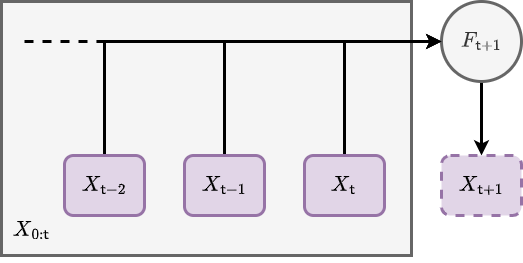
\includegraphics[width=10cm]{images/chapter-1-fundamental-loop.drawio.png}
\caption{Graph representation of Eq.~(\ref{eq:x-step-def}).}
\label{fig:fundamental-loop}
\end{figure}

The basic computational idea here is illustrated in Fig.~\ref{fig:fundamental-loop}; we iterate the matrix $X$ forward in time by a row, and use its previous version $X_{0:{\sf t}}$ as an entire matrix input into a function which populates the elements of its latest rows. In pseudocode you could easily write something with the same idea in it, and it would probably look something like the method diagram in Fig.~\ref{fig:fundamental-loop-code}.

\begin{figure}[h]
\centering
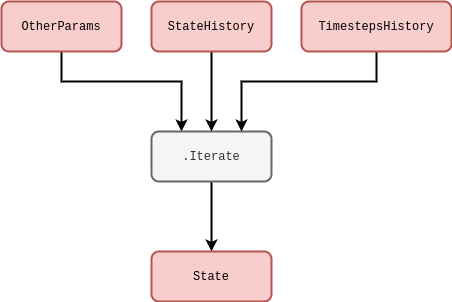
\includegraphics[width=10cm]{images/chapter-1-fundamental-loop-code.drawio.png}
\caption{Pseudocode representation of Eq.~(\ref{eq:x-step-def}).}
\label{fig:fundamental-loop-code}
\end{figure}

Pretty simple! But why go to all this trouble of storing matrix inputs for previous values of the same process? It's true that this is mostly redundant for \emph{Markovian} phenomena, i.e., processes where their only memory of their history is the most recent value they took. However, for a large class of stochastic processes a full memory\footnote{Or memory at least within some window.} of past values is essential to consistently construct the sample paths moving forward. This is true in particular for \emph{non-Markovian} phenomena, where the latest values don't just depend on the immediately previous ones but can depend on values which occured much earlier in the process as well.

For more complex physical models and integrators, the distinct notions of `numerical timestep' and `total elapsed continuous time' will crop up quite frequently. Hence, before moving on further details, it will be important to define the total elapsed time variable $t({\sf t})$ for processes which are defined in continuous time. Assuming that we have already defined some function $\delta t({\sf t})$ which returns the specific change in continuous time that corresponds to the step ${\sf t}-1 \rightarrow {\sf t}$, we will always be able to compute the total elapsed time through the relation
%%
\begin{align}
t({\sf t}) &= \sum^{{\sf t}}_{{\sf t}'=0}\delta t({\sf t}') \label{eq:t-steps-sum} \,.
\end{align}
%%
It's important to remember that our steps in continuous time may not be constant, so by defining the $\delta t({\sf t})$ function and summing over it we can enable this flexibility in the computation. In case the summation notation is no fun for programmers; we're simply adding up all of the differences in time to get a total.

So, now that we've mathematically defined a really general notion of iterating the stochastic process forward in time, it makes sense to discuss some simple examples. For instance, it is frequently possible to split $F$ up into deteministic (denoted $D$) and stochastic (denoted $S$) matrix-valued functions like so
%%
\begin{align}
& F^{i}_{{\sf t}+1}(X_{0:{\sf t}},z,{\sf t}) = D^{i}_{{\sf t}+1}(X_{0:{\sf t}},z,{\sf t}) + S^{i}_{{\sf t}+1}(X_{0:{\sf t}},z,{\sf t}) \,.
\end{align}
%%
In the case of stochastic processes with continuous sample paths, it's also nearly always the case with mathematical models of real-world systems that the deterministic part will at least contain the term $D^{i}_{{\sf t}+1}(X_{0:{\sf t}},z,{\sf t}) = X^i_{\sf t}$ because the overall system is described by some stochastic differential equation. This is not a really requirement in our general formalism, however.

What about the stochastic term? For example, if we wanted to consider a \emph{Wiener process noise}, we can define $W^i_{{\sf t}}$ is a sample from a Wiener process for each of the state dimensions indexed by $i$ and our formalism becomes
%%
\begin{align}
& S^{i}_{{\sf t}+1}(X_{0:{\sf t}},z,{\sf t}) = W^i_{{\sf t}+1}-W^i_{\sf t} \label{eq:wiener}\,.
\end{align}
%%
One draws the increments $W^i_{{\sf t}+1}-W^i_{\sf t}$ from a normal distribution with a mean of $0$ and a variance equal to the length of continuous time that the step corresponded to $\delta t({\sf t}+1)$, i.e., the probability density $P_{{\sf t}+1}(x^i)$ of the increments $x^i=W^i_{{\sf t}+1}-W^i_{\sf t}$ is
%%
\begin{align}
P_{{\sf t}+1}(x^i) &= {\sf NormalPDF}[x^i;0,\delta t({\sf t}+1)] \,.
\end{align}
%%
Note that for state spaces with dimensions $>1$, we could also allow for non-trivial cross-correlations between the noises in each dimension. In pseudocode, the Wiener process is schematically represented by Fig.~\ref{fig:wiener-process}.

\begin{figure}[h]
\centering
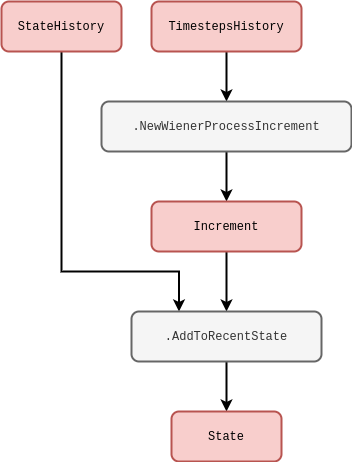
\includegraphics[width=8cm]{images/chapter-1-wiener-process.drawio.png}
\caption{Schematic of code for a Wiener process.}
\label{fig:wiener-process}
\end{figure}

In another example, to model \emph{geometric Brownian motion noise} we would simply have to multiply $X^i_{\sf t}$ to the Wiener process like so
%%
\begin{align}
& S^{i}_{{\sf t}+1}(X_{0:{\sf t}},z,{\sf t}) = X^i_{\sf t}(W^i_{{\sf t}+1}-W^i_{\sf t})\label{eq:gbm} \,.
\end{align}
%%
Here we have implicitly adopted the Itô interpretation to describe this stochastic integration. Given a carefully-defined integration scheme other interpretations of the noise would also be possible with our formalism too, e.g., Stratonovich\footnote{Which would implictly give $S^{i}_{{\sf t}+1}(X_{0:{\sf t}},z,{\sf t}) = (X^i_{{\sf t}+1}+X^i_{\sf t})(W^i_{{\sf t}+1}-W^i_{\sf t}) / 2$ for Eq.~(\ref{eq:gbm}).} or others within the more general `$\alpha$-family'~\cite{van1992stochastic,risken1996fokker,rog-will-2000}. The pseudocode for any of these should hoepfully be fairly straightforward to deduce based on the lines we've already written above.

\begin{figure}[h]
\centering
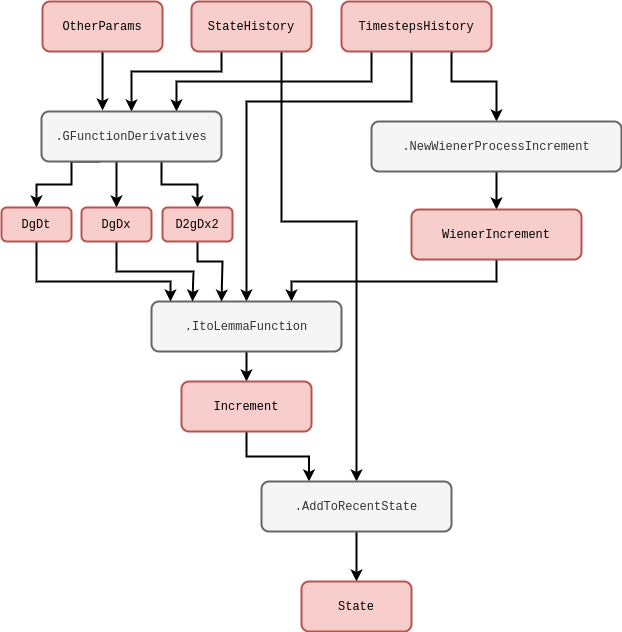
\includegraphics[width=12cm]{images/chapter-1-ito-lemma.drawio.png}
\caption{Schematic of code for Eq.~(\ref{eq:general-wiener}).}
\label{fig:ito-lemma}
\end{figure}

We can imagine even more general processes that are still Markovian. One example of these in a single-dimension state space would be to define the noise through some general function of the Wiener process like so
%%
\begin{align}
S^0_{{\sf t}+1}(X_{0:{\sf t}},z,{\sf t}) &= g[W^0_{{\sf t}+1},t({\sf t}+1)]-g[W^0_{\sf t}, t({\sf t})] \\
&= \bigg[ \frac{\partial g}{\partial t} + \frac{1}{2}\frac{\partial^2 g}{\partial x^2} \bigg] \delta t ({\sf t}+1) + \frac{\partial g}{\partial x} (W^0_{{\sf t}+1}-W^0_{\sf t}) \label{eq:general-wiener}\,,
\end{align}
%%
where $g(x,t)$ is some continuous function of its arguments which has been expanded out with Itô's Lemma on the second line. Note also that the computations in Eq.~(\ref{eq:general-wiener}) could be performed with numerical derivatives in principle, even if the function were extremely complicated. This is unlikely to be the best way to describe the process of interest, however, the mathematical expressions above can still be made a bit more meaningful to the programmer in this way. The pseudocode in general would look something like Fig.~\ref{fig:ito-lemma}.

Let's now look at a more complicated type of noise. For example, we might consider sampling from a \emph{fractional Brownian motion} process $[B_{H}]_{\sf t}$, where $H$ is known as the `Hurst exponent'. Following Ref.~\cite{decreusefond1999stochastic}, we can simulate this process in one of our state space dimensions by modifying the standard Wiener process by a fairly complicated integral factor which looks like this
%%
\begin{align}
S^{0}_{{\sf t}+1}(X_{0:{\sf t}},z,{\sf t}) &= \frac{(W^0_{{\sf t}+1} - W^0_{\sf t})}{\delta t({\sf t})}\int^{t({\sf t}+1)}_{t({\sf t})}{\rm d}t' \frac{(t'-t)^{H-\frac{1}{2}}}{\Gamma (H+\frac{1}{2})} {}_2F_1 \bigg( H-\frac{1}{2};\frac{1}{2}-H;H+\frac{1}{2};1-\frac{t'}{t}\bigg) \label{eq:fbm} \,,
\end{align}
%%
where $S^{0}_{{\sf t}+1}(X_{0:{\sf t}},z,{\sf t})=[B_{H}]_{{\sf t}+1}-[B_{H}]_{{\sf t}}$. The integral in Eq.~(\ref{eq:fbm}) can be approximated using an appropriate numerical procedure (like the trapezium rule, for instance). In the expression above, we have used the symbols ${}_2F_1$ and $\Gamma$ to denote the ordinary hypergeometric and gamma functions, respectively. A computational form of this integral is illustrated in Fig.~\ref{fig:fractional-brownian-motion} to try and disentangle some of the mathematics as a program.

\begin{figure}[h]
\centering
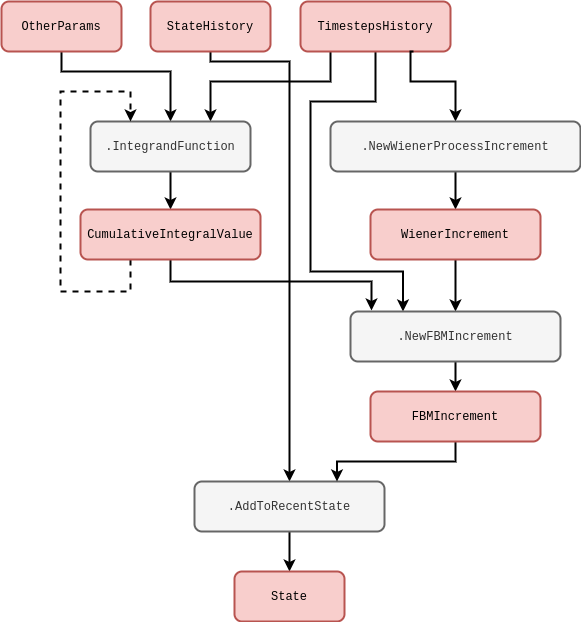
\includegraphics[width=11cm]{images/chapter-1-fractional-brownian-motion.drawio.png}
\caption{Schematic of code for Eq.~(\ref{eq:fbm}).}
\label{fig:fractional-brownian-motion}
\end{figure}

So far we have mostly been discussing noises with continuous sample paths, but we can easily adapt our computation to discontinuous sample paths as well. For instance, \emph{Poisson process noises} would generally take the form
%%
\begin{align}
S^{i}_{{\sf t}+1}(X_{0:{\sf t}},z,{\sf t}) &= [N_{\lambda}]^i_{{\sf t}+1}-[N_{\lambda}]^i_{\sf t}\,,
\end{align}
%%
where $[N_{\lambda}]^i_{\sf t}$ is a sample from a Poisson process with rate $\lambda$. One can think of this process as counting the number of events which have occured up to the given interval of time, where the intervals between each succesive event are exponentially distributed with mean $1/\lambda$. Such a simple counting process could be simulated exactly by explicitly setting a newly-drawn exponential variate to the next continuous time jump ${\delta t}({\sf t}+1)$ and iterating the counter. Other exact methods exist to handle more complicated processes involving more than one type of `event', such as the Gillespie algorithm~\cite{gillespie1977exact} --- though these techniques are not always be applicable in every situation.

Is using step size variation always possible? If we consider a \emph{time-inhomogeneous Poisson process noise}, which would generally take the form
%%
\begin{align}
S^{i}_{{\sf t}+1}(X_{0:{\sf t}},z,{\sf t}) &= [N_{\lambda ({\sf t}+1)}]^i_{{\sf t}+1}-[N_{\lambda ({\sf t})}]^i_{\sf t}\,,
\end{align}
%%
the rate $\lambda ({\sf t})$ has become a deterministically-varying function in time. In this instance, it likely not be accurate to simulate this process by drawing exponential intervals with a mean of $1/\lambda ({\sf t})$ because this mean could have changed by the end of the interval which was drawn. An alternative approach (which is more generally capable of simulating jump processes but is an approximation) first uses a small time interval $\tau$ such that the most likely thing to happen in this period is nothing, and then the probability of the event occuring is simply given by
%%
\begin{align}
p({\sf event}) &= \frac{\lambda ({\sf t})}{\lambda ({\sf t}) + \frac{1}{\tau}} \label{eq:rejection}\,.
\end{align}
%%
This idea can be applied to phenomena with an arbitrary number of events and works well as a generalised approach to event-based simulation, though its main limitation is worth remembering; in order to make the approximation good, $\tau$ often must be quite small and hence our simulator must churn through a lot of steps. From now on we'll refer to this well-known technique as the \emph{rejection method}. Fig.~\ref{fig:inhomogeneous-poisson} may also help to understand this concept from the programmer's perspective.

\begin{figure}[h]
\centering
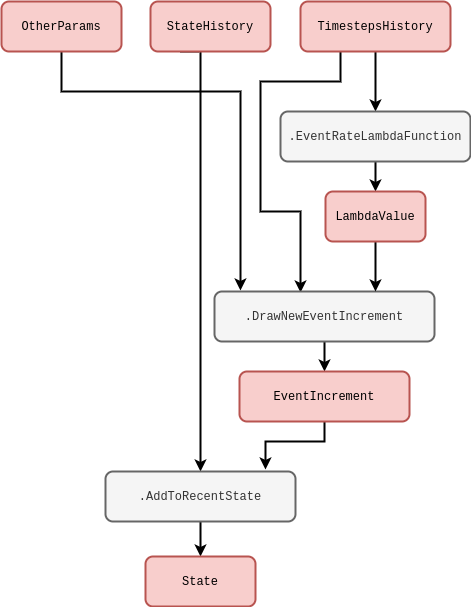
\includegraphics[width=9cm]{images/chapter-1-inhomogeneous-poisson.drawio.png}
\caption{Schematic of code for an inhomogeneous Poisson process.}
\label{fig:inhomogeneous-poisson}
\end{figure}

There are a few extensions to the simple Poisson process that introduce additional stochastic processes. \emph{Cox (doubly-stochastic) processes}, for instance, are basically where we replace the time-dependent rate $\lambda ({\sf t})$ with independent samples from some other stochastic process $\Lambda ({\sf t})$. For example, a Neyman-Scott process~\cite{neyman1958statistical} can be mapped as a special case of this because it uses a Poisson process on top of another Poisson process to create maps of spatially-distributed points. In our formalism, a two-state implementation of the Cox process noise would look like
%%
\begin{align}
S^{0}_{{\sf t}+1}(X_{0:{\sf t}},z,{\sf t}) &= \Lambda ({\sf t}+1) \\
S^{1}_{{\sf t}+1}(X_{0:{\sf t}},z,{\sf t}) &= [N_{S^{0}_{{\sf t}+1}}]^i_{{\sf t}+1}-[N_{S^{0}_{{\sf t}}}]^i_{\sf t}\,.
\end{align}
%%
This process could be simulated using the pseudocode we wrote for the time-inhomogeneous Poisson process previously --- where we would just replace \texttt{EventRateLambdaFunction} with a function that generates the stochastic rate $\Lambda ({\sf t})$.

Another extension is \emph{compound Poisson process noise}, where it's the count values $[N_{\lambda}]^i_{\sf t}$ which are replaced by independent samples $[J_{\lambda}]^i_{\sf t}$ from another probability distribution, i.e.,
%%
\begin{align}
S^{i}_{{\sf t}+1}(X_{0:{\sf t}},z,{\sf t}) &= [J_{\lambda}]^i_{{\sf t}+1}-[J_{\lambda}]^i_{\sf t}\,.
\end{align}
%%
Note that the rejection method of Eq.~(\ref{eq:rejection}) can be employed effectively to simulate any of these extensions as long as a sufficiently small $\tau$ is chosen. Once again, the pseudocode we wrote previously would be sufficient to simulate this process with one tweak: add into the \texttt{DrawNewEventIncrement} function the calling of a function which generates the $[J_{\lambda}]^i_{\sf t}$ samples and output these if the event occurs.

All of the examples we have discussed so far are Markovian. Given that we have explicitly constructed the formalism to handle non-Markovian phenomena as well, it would be worthwhile going some examples of this kind of process too. \emph{Self-exciting process noises} would generally take the form
%%
\begin{align}
S^{0}_{{\sf t}+1}(X_{0:{\sf t}},z,{\sf t}) &= {\cal I}_{{\sf t}+1} (X_{0:{\sf t}},z,{\sf t}) \\
S^{1}_{{\sf t}+1}(X_{0:{\sf t}},z,{\sf t}) &= [N_{S^{0}_{{\sf t}+1}}]^i_{{\sf t}+1}-[N_{S^{0}_{{\sf t}}}]^i_{\sf t} \,,
\end{align}
%%
where the stochastic rate ${\cal I}_{{\sf t}+1} (X_{0:{\sf t}},z,{\sf t})$ now depends on the history explicitly. Amongst other potential inputs we can see, e.g., Hawkes processes~\cite{hawkes1971spectra} as an example of above by substituting 
%%
\begin{align}
{\cal I}_{{\sf t}+1} (X_{0:{\sf t}},z,{\sf t}) &= \mu + \sum^{{\sf t}}_{{\sf t}'=0}\gamma [t({\sf t})-t({\sf t}')]S^{1}_{{\sf t}'} \,,
\end{align}
%%
where $\gamma$ is the `exciting kernel' and $\mu$ is some constant background rate. In order to simulate a Hawkes process using our formalism, the pseudocode would be something like Fig.~\ref{fig:hawkes-process}.

\begin{figure}[h]
\centering
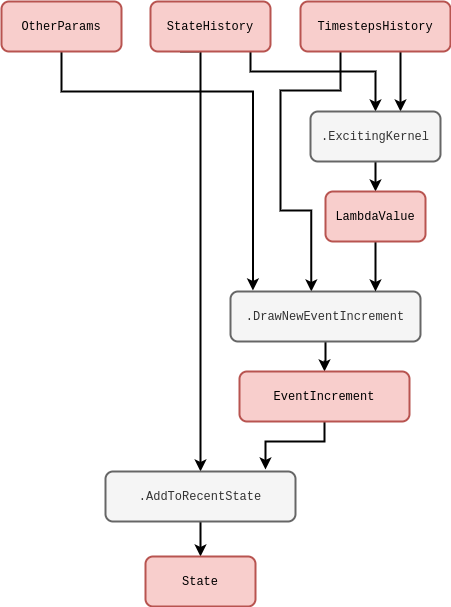
\includegraphics[width=9cm]{images/chapter-1-hawkes-process.drawio.png}
\caption{Schematic of code for a Hawkes process.}
\label{fig:hawkes-process}
\end{figure}

Note that this idea of integration kernels could also be applied back to our Wiener process. For example, another type of non-Markovian phenomenon that frequently arises across physical and life systems integrates the Wiener process history like so
%%
\begin{align}
S^{0}_{{\sf t}+1}(X_{0:{\sf t}},z,{\sf t}) &= W^0_{{\sf t}+1}-W^0_{\sf t}\\
S^{1}_{{\sf t}+1}(X_{0:{\sf t}},z,{\sf t}) &= u\sum^{{\sf t}}_{{\sf t}'=0}e^{-u[t({\sf t})-t({\sf t}')]} S^{0}_{{\sf t}'}\,,
\end{align}
%%
where $u$ is inversely proportional to the length of memory in continuous time.

\section{\sffamily Software design}

So we've proposed a computational formalism and then studied it in more detail to demonstrate that it can cope with a variety of different stochastic phenomena. Now we're ready to summarise what we want the stochadex software package to be able to do. But what's so complicated about Eq.~(\ref{eq:x-step-def})? Can't we just implement an iterative algorithm with a single function? It's true that the fundamental concept is very straightforward, but as we'll discuss in due course; the stochadex needs to have a lot of configurable features so that it's applicable in different situations. Ideally, the stochadex sampler should be designed to try and maintain a balance between performance and flexibility of utilisation.

If we begin with the obvious first set of criteria; we want to be able to freely configure the iteration function $F$ of Eq.~(\ref{eq:x-step-def}) and the timestep function $t$ of Eq.~(\ref{eq:t-steps-sum}) so that any process we want can be described. The point at which a simulation stops can also depend on some algorithm termination condition which the user should be able to specify up-front.

\begin{figure}[h]
\centering
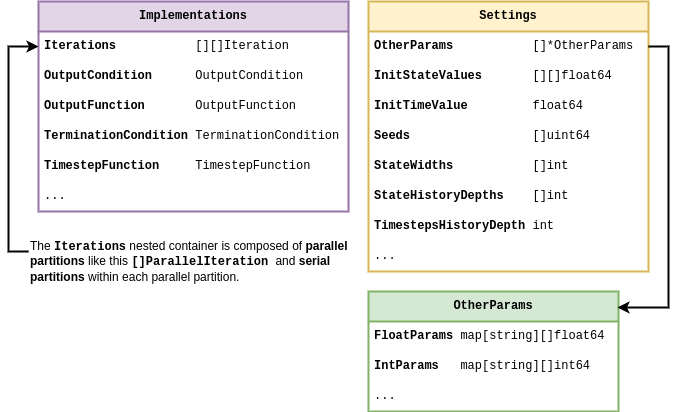
\includegraphics[width=13cm]{images/chapter-1-stochadex-data-types.drawio.png}
\caption{A relational summary of the configuration data types in the stochadex.}
\label{fig:data-types-design}
\end{figure}

Once the user has written the code to create these functions for the stochadex, we want to then be able to recall them in future only with configuration files while maintaining the possibility of changing their simulation run parameters. This flexibility should facilitate our uses for the simulation later in the book, and from this perspective it also makes sense that the parameters should include the random seed and initial state value.

The state history matrix $X$ should be configurable in terms of its number of rows --- what we'll call the `state width' --- and its number of columns --- what we'll call the `state history depth'. If we were to keep increasing the state width up to millions of elements or more, it's likely that on most machines the algorithm performance would grind to a halt when trying to iterate over the resulting $X$ within a single thread. Hence, before the algorithm or its performance in any more detail, we can pre-empt the requirement that $X$ should represented in computer memory by a set of partitioned matrices which are all capable of communicating to one-another downstream. In this paradigm, we'd like the user to be able to configure which state partitions are able to communicate with each other without having to write any new code.

For convenience, it seems sensible to also make the outputs from stochadex runs configurable. A user should be able to change the form of output that they want through, e.g., some specified function of $X$ at the time of outputting data. The times that the stochadex should output this data can also be decided by some user-specified condition so that the frequency of output is fully configurable as well. 

In summary, we've put together a schematic of configuration data types and their relationships in Fig.~\ref{fig:data-types-design}. In this diagram there is some indication of the data type that we propose to store each piece information in (in Go syntax), and the diagram as a whole should serve as a useful guide to the basic structure of configuration files for the stochadex.

It's clear that in order to simulate Eq.~(\ref{eq:x-step-def}), we need an interative algorithm which reapplies a user-specified function to the continually-updated history. But let's now return to the point we made earlier about how the performance of such an algorithm will depend on the size of the state history matrix $X$. The key bit of the algorithm design that isn't so straightforward is: how do we sucessfully split this state history up into separate partitions in memory while still enabling them to communicate effectively with each other? Other generalised simulation frameworks --- such as SimPy~\cite{simpy}, StoSpa~\cite{stospa} and FLAME GPU~\cite{flamegpu} --- have all approached this problem in different ways, and with different software architectures. 

In Fig.~\ref{fig:loop-design} we've illustrated what a loop involving separate state partitions looks like in the stochadex simulator. Each partition is handled by concurrently running execution threads of the same process, while a separate process may be used to handle the outputs from the algorithm. As the diagram shows, the main sequence of each loop iteration follows the pattern: 
%%
\begin{enumerate}
\item{The \texttt{PartitionCoordinator} requests more iterations from each state partition by sending an \texttt{IteratorInputMessage} to a concurrently running goroutine.}
\item{The \texttt{StateIterator} in each goroutine executes the iteration and stores the resulting state update in a variable.}
\item{Once all of the iterations have been completed, the \texttt{PartitionCoordinator} then requests each goroutine to update its relevant partition of the state history by sending another \texttt{IteratorInputMessage} to each.}
\end{enumerate}
%%
This pattern ensures that no partition has access to values in the state history which are out of sync with its current state in time, and hence prevents anachronisms from occuring in the overall state iteration. 

\begin{figure}[h]
\centering
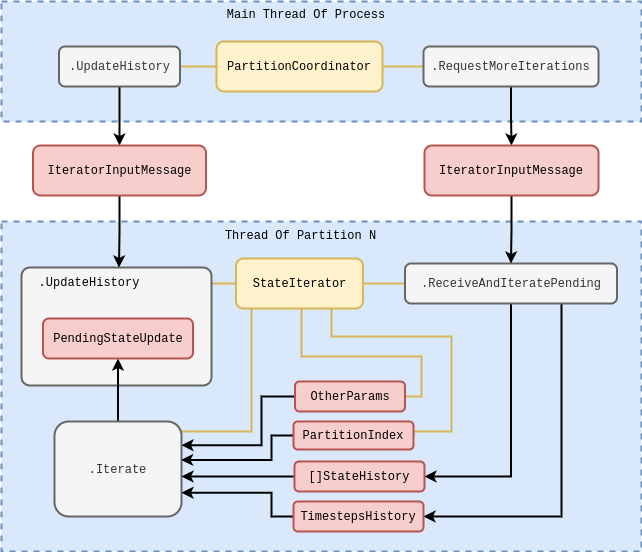
\includegraphics[width=13cm]{images/chapter-1-stochadex-loop.drawio.png}
\caption{Schematic for a step of the stochadex simulation algorithm.}
\label{fig:loop-design}
\end{figure}

It's also worth noting that while Fig.~\ref{fig:loop-design} illustrates only a single process; it's obviously true that we may run many of these whole diagrams at once to parallelise generating independent realisations of the simulation, if necessary.

As we stated at the beginning of this chapter: the full implementation of the stochadex can be found on GitHub by following this link: \href{https://github.com/umbralcalc/stochadex}{https://github.com/umbralcalc/stochadex}. Users can build the main binary executable of this repository and determine what configuration of the stochadex they would like to have through config at runtime (one can infer these configurations from Fig.~\ref{fig:data-types-design}). As Go is a statically typed language, this level of flexibility has been achieved using code templating proceeding runtime build and execution via \texttt{go run} `under-the-hood'. Users who find this particular execution pattern undesirable can also use all of the stochadex types, tools and methods as part of a standard library import.

In order to debug the simulation code and gain a more intuitive understanding of the outputs from a model as it is being developed, we have also written a lightweight frontend dashboard React~\cite{react} app in TypeScript to visualise any stochadex simulation as it is running. This dashboard can be launched by passing config at runtime to the main stochadex executable, and we have illustrated how all this fits together in a flowchart shown in Fig.~\ref{fig:stochadex-main}.

\begin{figure}[h]
\centering
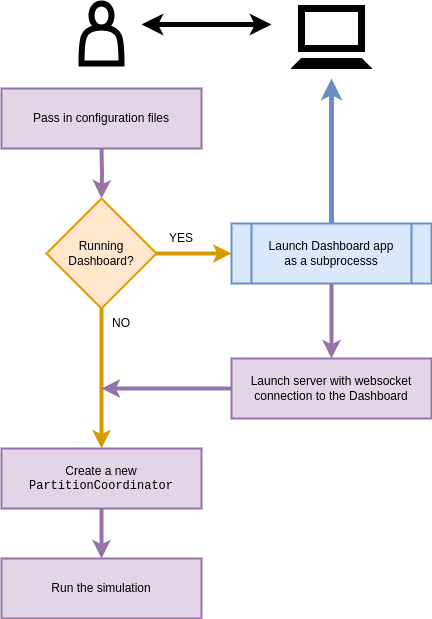
\includegraphics[width=9cm]{images/chapter-1-stochadex-main.drawio.png}
\caption{A diagram of the main stochadex binary executable.}
\label{fig:stochadex-main}
\end{figure}



\chapter{\sffamily Probabilistic learning methods}

{\bfseries\sffamily Concept.} To extend the formalism that we developed in the previous chapter to describe the time evolution of state probabilities. Having introduced the basic concepts, we then use this formalism to motivate some important methods for probabilistic learning. In particular, we will see how Gaussian processes regression and `empirical probabilistic reweighting' work, as well as discuss how some phenomena permit a convenient description via `mean-field' equations or regression of distribution moments. For the mathematically-inclined, this chapter will take a detailed look at how our formalism can be extended to focus on the time evolution of probabilities, with a view to probabilistic learning later on. For the programmers, this chapter will mostly focus on the algorithm concepts, but all of the relevant software lives in this public Git repository: \href{https://github.com/umbralcalc/learndadex}{https://github.com/umbralcalc/learnadex}.

\section{\sffamily Probabilistic formalism} 

This book is about building more realistic training environments for machine learning systems in the real world. In the last chapter we formalised, designed and built a generalised simulation engine which could serve as the essential scaffolding for these environments. So why then, in this chapter, do we want to extend our formalism to talk about probabilistic learning methods?

For many of these realistic environments where only partial state observations are possible, probabilistic learning tools can immediately become an essential tool to robustly infer the state of a system and predict its future states from any given point in time. Given that these tools are often so important for extending the capability of learning algorithms to deal with partially-observed domains; we propose to extend the idea of what is more conventionally considered a `machine learning environment' to include tools for system state inference and future state prediction. In this sense, this chapter, and the remaining chapters of {\bfseries\sffamily Part 1} in this book, will consider probabilistic learning as an essential part of the environment for a machine learning system.

In this chapter, we're going to discuss the formal connections between some probabilistic learning methods and the simulation formalism we introduced in the last chapter. The novelties in this chapter are less to do with the probabilistic learning methodology and lie more in the specifics of how we combine some of these ideas together when referencing the stochadex formalism, and how this manifests in designing more generally-applicable software for the user.

Let's start by returning to the formalism that we introduced in the previous chapter. As we discussed at that point; this formalism is appropriate for sampling from nearly every stochastic phenomenon that one can think of. We are going to extend this description to consider what happens to the probability that the state history matrix takes a particular set of values over time.

\begin{figure}[h]
\centering
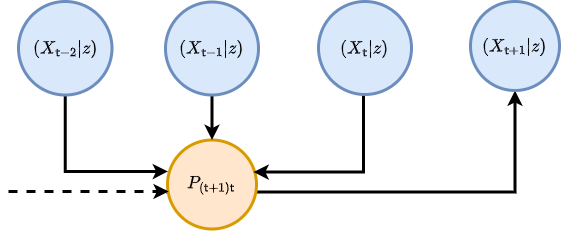
\includegraphics[width=12cm]{images/chapter-2-master-eq-graph.drawio.png}
\caption{Graph representation of Eq.~(\ref{eq:master-x-cont}).}
\label{fig:master-eqn}
\end{figure} 

So, how do we begin? In the first chapter, we defined the general stochastic process with the formula $X^{i}_{{\sf t}+1} = F^{i}_{{\sf t}+1}(X_{0:{\sf t}},z,{\sf t})$. This equation also has an implicit \emph{master equation} associated to it that fully describes the time evolution of the \emph{probability density function} $P_{{\sf t}+1}(X\vert z)$ of $X_{0:{\sf t}+1}=X$ given that the parameters of the process are $z$. This can be written as
%%
\begin{align}
P_{{\sf t}+1}(X\vert z) &= P_{{\sf t}}(X'\vert z) P_{({\sf t}+1){\sf t}}(x\vert X',z) \label{eq:master-x-cont}\,,
\end{align}
%%
where for the time being we are assuming the state space is continuous in each of the matrix elements and $P_{({\sf t}+1){\sf t}}(x\vert X',z)$ is the conditional probability that $X_{{\sf t}+1}=x$ given that $X_{0:{\sf t}}=X'$ at time ${\sf t}$ and the parameters of the process are $z$. To try and understand what Eq.~(\ref{eq:master-x-cont}) is saying, we find it's helpful to think of an iterative relationship between probabilities; each of which is connected by their relative conditional probabilities. We've also illustrated this kind of thinking in Fig.~\ref{fig:master-eqn}.

Consider what happens when we extend the chain of conditional probabilities in Eq.~(\ref{eq:master-x-cont}) back in time by one step. In doing so, we retrieve a joint probability of rows $X_{{\sf t}+1}=x$ and $X_{{\sf t}}=x'$ on the right hand side of the expression 
%%
\begin{align}
P_{{\sf t}+1}(X\vert z) &= P_{{\sf t}-1}(X''\vert z) P_{({\sf t}+1){\sf t}({\sf t}-1)}(x,x'\vert X'',z) \label{eq:master-x-pairwise-joint}\,.
\end{align}
%%
Since Eqs.~(\ref{eq:master-x-cont}) and~(\ref{eq:master-x-pairwise-joint}) are both valid ways to obtain $P_{{\sf t}+1}(X\vert z)$ we can average between them without loss of generality in the original expression, like this
%%
\begin{align}
P_{{\sf t}+1}(X\vert z) &= \frac{1}{2}\big[ P_{{\sf t}}(X'\vert z) P_{({\sf t}+1){\sf t}}(x\vert X',z) + P_{{\sf t}-1}(X''\vert z) P_{({\sf t}+1){\sf t}({\sf t}-1)}(x,x'\vert X'',z) \big]\,.
\end{align}
%%
Following this line of reasoning to its natural conclusion, Eq.~(\ref{eq:master-x-cont}) can hence be generalised to consider all possible joint distributions of rows at different timesteps like this
%%
\begin{align}
P_{{\sf t}+1}(X\vert z) &= \frac{1}{{\sf t}}\sum_{{\sf t}''=0}^{{\sf t}}P_{{\sf t}''}(X''\vert z) P_{({\sf t}+1){\sf t}\dots{\sf t}''}(x,x',\dots \vert X'',z) \label{eq:master-x-cont-sum-gen}\,.
\end{align}
%%

If we wanted to just look at the distribution over the latest row $X_{{\sf t}+1}=x$, we could achieve this through marginalisation over all of the previous matrix rows in Eq.~(\ref{eq:master-x-cont}) like this
%%
\begin{align}
P_{{\sf t}+1}(x\vert z) = \int_{\Omega_{{\sf t}}}{\rm d}X' P_{{\sf t}+1}(X\vert z) &= \int_{\Omega_{{\sf t}}}{\rm d}X' P_{{\sf t}}(X'\vert z) P_{({\sf t}+1){\sf t}}(x\vert X',z) \label{eq:master-x-cont-latest-row} \,.
\end{align}
%%
But what is $\Omega_{\sf t}$? You can think of this as just the domain of possible matrix $X'$ inputs into the integral which will depend on the specific stochastic process we are looking at. 

The symbol ${\rm d}X'$ in Eq.~(\ref{eq:master-x-cont-latest-row}) is our shorthand notation throughout the book for computing the sum of integrals over previous state history matrices which can further be reduced via Eq.~(\ref{eq:master-x-cont-sum-gen}) into a product of sub-domain integrals over each matrix row
%%
\begin{align}
P_{{\sf t}+1}(x\vert z) &= \frac{1}{{\sf t}}\sum_{{\sf t}''=0}^{{\sf t}} \bigg\lbrace \int_{\omega_{{\sf t}'}}{\rm d}^nx'...\int_{\Omega_{{\sf t}''}}{\rm d}X'' \bigg\rbrace \,P_{{\sf t}''}(X''\vert z) P_{({\sf t}+1){\sf t}\dots{\sf t}''}(x,x',... \vert X'',z) \\
&= \frac{1}{{\sf t}}\sum_{{\sf t}''=0}^{{\sf t}} \int_{\Omega_{{\sf t}''}}{\rm d}X'' P_{{\sf t}''}(X''\vert z) P_{({\sf t}+1){\sf t}''}(x \vert X'',z) \label{eq:master-x-cont-latest-row-gen} \,,
\end{align}
%%
where each row measure is a Cartesian product of $n$ elements (a Lebesgue measure), i.e.,
%%
\begin{align}
{\rm d}^nx = \prod_{i=0}^n{\rm d}x^i \,,
\end{align}
%%
and lowercase $x, x', \dots$ values will always refer to individual rows within the state matrices. Note that $1/{\sf t}$ here is a normalisation factor --- this just normalises the sum of all probabilities to 1 given that there is a sum over ${\sf t}'$. Note also that, if the process is defined over continuous time, we would need to replace 
%%
\begin{align}
\frac{1}{{\sf t}}\sum_{{\sf t}'=0}^{{\sf t}} \rightarrow \frac{1}{t({\sf t})}\sum_{{\sf t}'=0}^{{\sf t}}\delta t({\sf t}') \,.
\end{align}
%%

Let's go through some examples. Non-Markovian phenomena with continuous state spaces can have quite complex master equations. A relatively simple example is that of pure diffusion processes which exhibit stochastic resetting at a rate $r$ to a remembered location from the trajectory history~\cite{boyer2017long}
%%
\begin{align}
P_{{\sf t}+1}(x\vert z) &= (1-r)P_{{\sf t}}(x\vert z) + \sum_{i=0}^n\sum_{j=0}^n\frac{\partial}{\partial x^i}\frac{\partial}{\partial x^j}\bigg[ D_{{\sf t}}(x,z)P_{{\sf t}}(x\vert z) \bigg] + r\sum_{{\sf t}'=0}^{{\sf t}}\delta t ({\sf t}')K[t({\sf t}){-}t({\sf t}')]P_{{\sf t}'}(x\vert z) \,,
\end{align}
%%
where here $K$ is some memory kernel. For Markovian phenomena which have a continuous state space, Eqs.~(\ref{eq:master-x-cont}) and~(\ref{eq:master-x-cont-latest-row}) no longer depend on timesteps older than the immediately previous one, hence, e.g., Eq.~(\ref{eq:master-x-cont-latest-row}) reduces to just
%%
\begin{align}
P_{{\sf t}+1}(x\vert z) &= \int_{\omega_{\sf t}}{\rm d}^nx' \, P_{\sf t}(x'\vert z) P_{({\sf t}+1){\sf t}}(x\vert x',z) \label{eq:master-x-cont-markov} \,.
\end{align}
%%
A famous example of this kind of phenomenon arises from approximating Eq.~(\ref{eq:master-x-cont-markov}) with an expansion (Kramers-Moyal~\cite{kramers1940brownian, moyal1949stochastic}) up to second-order, yielding the Fokker-Planck equation 
%%
\begin{align}
P_{{\sf t}+1}(x\vert z) &= P_{{\sf t}}(x\vert z) - \sum_{i=0}^n\frac{\partial}{\partial x^i}\bigg[ \mu_{{\sf t}}(x,z)P_{{\sf t}}(x\vert z)\bigg] + \sum_{i=0}^n\sum_{j=0}^n\frac{\partial}{\partial x^i}\frac{\partial}{\partial x^j}\bigg[ D_{{\sf t}}(x,z)P_{{\sf t}}(x\vert z) \bigg] \,,
\end{align}
%%
which describes a process undergoing drift-diffusion.

An analog of Eq.~(\ref{eq:master-x-cont-latest-row}) exists for discrete state spaces as well. We just need to replace the integral with a sum and the schematic would look something like this
%%
\begin{align}
P_{{\sf t}+1}(x\vert z) &= \sum_{\Omega_{{\sf t}}} P_{{\sf t}}(X'\vert z) P_{({\sf t}+1){\sf t}}(x \vert X', z) \label{eq:master-x-disc} \,,
\end{align}
%%
where we note that the $P$'s in the expression above all now refer to \emph{probability mass functions}. In what follows, discrete state space can always be considered by replacing the integrals with summations over probability masses in this manner; we only use the continuous state space formulation for our notation because one could argue it's a little more general. 

Analogously to continuous state spaces, we can give some examples of master equations for phenomena with a discrete state space as well. In the Markovian case, we need look no further than a simple time-dependent Poisson process
%%
\begin{align}
P_{{\sf t}+1}(x\vert z) &= \lambda ({\sf t}) \delta t({\sf t}{+}1)P_{{\sf t}}(x{-}1\vert z) + \big[1-\lambda ({\sf t}) \delta t({\sf t}{+}1)\big] P_{{\sf t}}(x\vert z) \,.
\end{align}
%%
For such an example of a non-Markovian system, a Hawkes process~\cite{hawkes1971spectra} master equation would look something like this
%%
\begin{align}
P_{{\sf t}+1}(x\vert z) &= \mu \delta t({\sf t}{+}1)P_{{\sf t}}(x{-}1\vert z) + \big[ 1-\mu \delta t({\sf t}{+}1)\big] P_{{\sf t}}(x\vert z) \nonumber \\
& + \sum_{x'=0}^\infty\sum_{{\sf t}'=0}^{{\sf t}} \phi [t({\sf t})-t({\sf t}')] \delta t({\sf t}{+}1)P_{{\sf t}{\sf t}'({\sf t}'-1)}(x{-}1,x',x'{-}1\vert z) \nonumber \\
&+ \sum_{x'=0}^\infty\bigg\lbrace 1-\sum_{{\sf t}'=0}^{{\sf t}} \phi [t({\sf t})-t({\sf t}')] \delta t({\sf t}{+}1)\bigg\rbrace P_{{\sf t}{\sf t}'({\sf t}'-1)}(x, x', x'{-}1\vert z) \,,
\end{align}
%%
where we note the complexity in this expression arises because it has to include a coupling between the rate at which events occur and an explicit memory of when the previous ones did occur (recorded by differencing the count between adjacent timesteps by 1).

\section{\sffamily Motivating probabilistic learning}

So now that we are more familiar with the notation used by Eq.~(\ref{eq:master-x-cont-latest-row}), we can use it to motivate some useful probabilistic learning methods. While it's worth going into some mathematical detail to give a better sense of where each technique comes from, we should emphasise that the methodologies we discuss here are not new to the technical literature at all. We draw on influences from Empirical Dynamical Modeling (EDM)~\cite{sugihara1990nonlinear}, some classic nonparametric local regression techniques --- such as LOWESS/Savitzky-Golay filtering~\cite{savitzky1964smoothing} --- and also Gaussian processes~\cite{murphy2012machine}.  

Let's begin our discussion of algorithms by integrating Eq.~(\ref{eq:master-x-cont-latest-row}) over $x$ to obtain a relation for the mean of the distribution
%%
\begin{align}
M_{{\sf t}+1}(z) &= \int_{\omega_{{\sf t}+1}}{\rm d}^nx \,x\, P_{{\sf t}+1}(x\vert z) = \frac{1}{{\sf t}}\sum_{{\sf t}''=0}^{{\sf t}} \int_{\Omega_{{\sf t}''}}{\rm d}X'' P_{{\sf t}''}(X''\vert z) M_{({\sf t}+1){\sf t}''}(X'',z) \label{eq:mean-field-master}\,,
\end{align}
%%
where you can view the $M_{({\sf t}+1){\sf t}''}(X'',z)$ values as either terms in some regression model, or derivable explicitly from a known master equation. The latter of these provides one approach to statistically infer the states and parameters of stochastic simulations from data: one begins by knowing what the master equation is, uses this to compute the time evolution of the mean (and potentially higher-order statistics) and then connects these ${\sf t}$ and $z$-dependent statistics back to the likelihood of observing the data. This is what is commonly known as the `mean-field' inference approach; averaging over the available degrees of freedom in the statistical moments of distributions. Though, knowing what the master equation is for an arbitrarily-defined stochastic phenomenon can be very difficult indeed, and the resulting equations typically require some form of approximation. 

\begin{figure}[h]
\centering
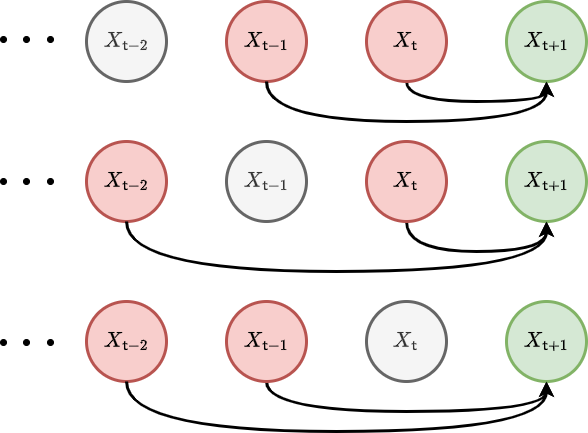
\includegraphics[width=8cm]{images/chapter-2-second-temporal-correlation.drawio.png}
\caption{A graph representation of the correlations in Eq.~(\ref{eq:second-order-correl}).}
\label{fig:second-temporal-correlation}
\end{figure} 

Given that the mean-field approach isn't always going to be viable as an inference method, we should also consider other ways to describe the shape and time evolution characteristics of $P_{{\sf t}+1}(X\vert z)$. For continuous state spaces, it's possible to approximate this whole distribution with a logarithmic expansion like so
%%
\begin{align}
\ln P_{{\sf t}+1}(X\vert z) &\simeq \ln P_{{\sf t}+1}(X_*\vert z) + \frac{1}{2}\sum_{{\sf t}'=0}^{{\sf t}+1}\sum_{i=0}^{n}\sum_{j=0}^{n} (x-x_*)^i {\cal H}^{ij}_{({\sf t}+1){\sf t}'}(z) (x'-x'_*)^j \label{eq:second-order-log-expansion} \\
{\cal H}^{ij}_{({\sf t}+1){\sf t}'}(z) &= \frac{\partial}{\partial x^i}\frac{\partial}{\partial (x')^j}\ln P_{{\sf t}+1}(X\vert z) \bigg\vert_{X=X_*} \label{eq:second-order-log-expansion-kernel} \,,
\end{align}
%% 
where the values for $X_*$ (and its rows $x_*, x_*', \dots$) are defined by the vanishing of the first derivative, i.e., these are chosen such that
%%
\begin{align}
\frac{\partial}{\partial x^i}\ln P_{{\sf t}+1}(X\vert z) \bigg\vert_{X=X_*} &= 0 \,.
\end{align}
%%
This logarithmic expansion is one way to see how a Gaussian process regression is able to approximate $X_{{\sf t}}$ evolving in time for many different processes. By selecting the appropriate function for the kernel given by Eq.~(\ref{eq:second-order-log-expansion-kernel}), a Gaussian process regression can be fully specified.

If we keep the truncation up to second order in Eq.~(\ref{eq:second-order-log-expansion}), note that this expression implies a pairwise correlation structure of the form
%%
\begin{align}
P_{{\sf t}+1}(X\vert z) &\rightarrow \prod_{{\sf t}'=0}^{{\sf t}}P_{({\sf t}+1){\sf t}'}(x,x'\vert z) = \prod_{{\sf t}'=0}^{{\sf t}}P_{{\sf t}'}(x'\vert z)P_{({\sf t}+1){\sf t}'}(x\vert x', z) \,.
\end{align}
%%
Given this pairwise temporal correlation structure, Eq.~(\ref{eq:master-x-cont-latest-row-gen}) reduces to this simpler sum of integrals
%%
\begin{align}
P_{{\sf t}+1}(x\vert z) &= \frac{1}{{\sf t}}\sum_{{\sf t}'=0}^{{\sf t}}\int_{\omega_{{\sf t}'}}{\rm d}^nx' P_{{\sf t}'}(x'\vert z)P_{({\sf t}+1){\sf t}'}(x\vert x',z) \label{eq:second-order-correl} \,.
\end{align}
%%
We have illustrated these second-order correlations with a graph visualisation in Fig.~(\ref{fig:second-temporal-correlation}).

\begin{figure}[h]
\centering
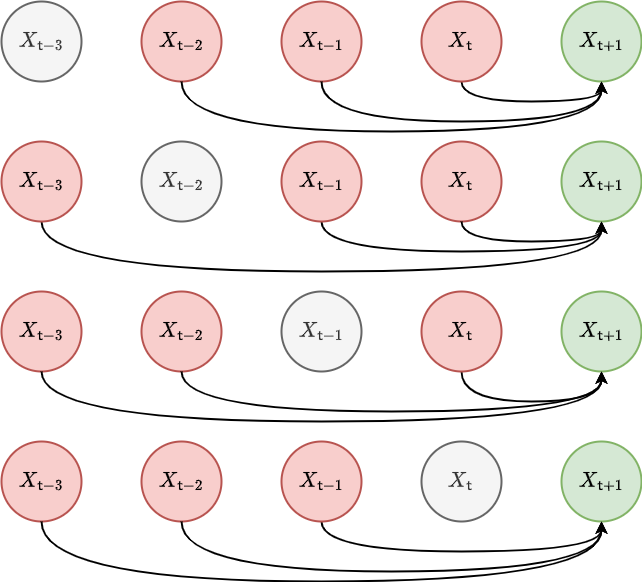
\includegraphics[width=10cm]{images/chapter-2-third-temporal-correlation.drawio.png}
\caption{A graph representation of the correlations in Eq.~(\ref{eq:third-order-correl}).}
\label{fig:third-temporal-correlation}
\end{figure}

In a similar fashion, we can increase the expansion order of Eq.~(\ref{eq:second-order-log-expansion}) to include third-order correlations such that 
%%
\begin{align}
P_{{\sf t}+1}(X\vert z) &\rightarrow \prod_{{\sf t}'=0}^{{\sf t}}\prod_{{\sf t}''=0}^{{\sf t}'-1} P_{{\sf t}'{\sf t}''}(x',x''\vert z)P_{({\sf t}+1){\sf t}'{\sf t}''}(x\vert x',x'',z) \,,
\end{align}
%%
and, in this instance, one can show that Eq.~(\ref{eq:master-x-cont-latest-row-gen}) reduces to
%%
\begin{align}
P_{{\sf t}+1}(x\vert z) &= \frac{1}{{\sf t}}\sum_{{\sf t}'=0}^{{\sf t}}\frac{1}{{\sf t}'-1}\sum_{{\sf t}''=0}^{{\sf t}'-1}\int_{\omega_{{\sf t}'}}{\rm d}^nx'\int_{\omega_{{\sf t}''}}{\rm d}^nx'' P_{{\sf t}'{\sf t}''}(x',x''\vert z)P_{({\sf t}+1){\sf t}'{\sf t}''}(x\vert x',x'',z) \label{eq:third-order-correl} \,.
\end{align}
%%
We have also illustrated these third-order correlations with another graph visualisation in Fig.~(\ref{fig:third-temporal-correlation}). Using $P_{{\sf t}'{\sf t}''}(x',x''\vert z) = P_{{\sf t}''}(x''\vert z) P_{{\sf t}'{\sf t}''}(x'\vert x'', z)$ one can also show that this integral is a marginalisation of this expression
%%
\begin{align}
P_{({\sf t}+1){\sf t}''}(x\vert x'', z) &= \frac{1}{{\sf t}}\sum_{{\sf t}'=0}^{{\sf t}}\int_{\omega_{{\sf t}'}}{\rm d}^nx'P_{{\sf t}'{\sf t}''}(x'\vert x'',z)P_{({\sf t}+1){\sf t}'{\sf t}''}(x\vert x',x'',z) \,,
\end{align}
%%
which describes the time evolution of the conditional probabilities. Note how this implies that the Gaussian process kernel itself can be evolved through time to replicate these higher-order temporal correlations for a regression problem, if desired.

Another probabilistic learning algorithm that we can consider is what we shall call `empirical probabilistic reweighting'. There is another expression for the mean of the distribution, that we can derive under certain conditions, which will be valuable to motivating this algorithm. If the probability distribution over each row of the state history matrix is \emph{stationary} --- meaning that $P_{{\sf t}+1}(x\vert z)=P_{{\sf t}'}(x\vert z)$ --- it's possible to go one step further than Eq.~(\ref{eq:mean-field-master}) and assert that
%%
\begin{align}
M_{{\sf t}+1}(z) &= \int_{\omega_{{\sf t}+1}}{\rm d}^nx \,x\,P_{{\sf t}+1}(x\vert z) = \frac{1}{{\sf t}}\sum_{{\sf t}'=0}^{{\sf t}}\int_{\omega_{{\sf t}'}}{\rm d}^nx' \,x'\, P_{{\sf t}'}(x'\vert z) \int_{\omega_{{\sf t}+1}}{\rm d}^nx\, P_{({\sf t}+1){\sf t}'}(x\vert x',z) \label{eq:stationary-mean-estimator}\,.
\end{align}
%%

To see that Eq.~(\ref{eq:stationary-mean-estimator}) is true, first note that a joint distribution over both $x$ and $x'$ can be derived like this $P_{({\sf t}+1){\sf t}'}(x,x'\vert z)=P_{({\sf t}+1){\sf t}'}(x\vert x',z)P_{{\sf t}'}(x'\vert z)$. Secondly, note that this joint distribution will always allow variable swaps trivially like this $P_{({\sf t}+1){\sf t}'}(x,x'\vert z)=P_{{\sf t}'({\sf t}+1)}(x',x\vert z)$. Then, lastly, note that stationarity of $P_{{\sf t}+1}(x\vert z)=P_{{\sf t}'}(x\vert z)$ means 
%%
\begin{align}
\frac{1}{{\sf t}}\sum_{{\sf t}'=0}^{{\sf t}}\int_{\omega_{{\sf t}+1}} {\rm d}^nx\int_{\omega_{{\sf t}'}} {\rm d}^nx' \,x\, P_{({\sf t}+1){\sf t}'}(x,x'\vert z)&=\frac{1}{{\sf t}}\sum_{{\sf t}'=0}^{{\sf t}}\int_{\omega_{{\sf t}'}} {\rm d}^nx\int_{\omega_{{\sf t}+1}} {\rm d}^nx' \,x\, P_{{\sf t}'({\sf t}+1)}(x,x'\vert z)\nonumber \\
&=\frac{1}{{\sf t}}\sum_{{\sf t}'=0}^{{\sf t}}\int_{\omega_{{\sf t}'}} {\rm d}^nx'\int_{\omega_{{\sf t}+1}} {\rm d}^nx \,x'\, P_{({\sf t}+1){\sf t}'}(x,x'\vert z) \nonumber \\
&=\frac{1}{{\sf t}}\sum_{{\sf t}'=0}^{{\sf t}}\int_{\omega_{{\sf t}'}}{\rm d}^nx' \,x'\, P_{{\sf t}'}(x'\vert z) \int_{\omega_{{\sf t}+1}}{\rm d}^nx\, P_{({\sf t}+1){\sf t}'}(x\vert x',z)\nonumber \,,
\end{align}
%%
where we've used the trivial variable swap and integration variable relabelling to arrive at the second equality in the expressions above. 

The standard covariance matrix elements can also be computed in a similar fashion
%%
\begin{align}
C^{ij}_{{\sf t}+1}(z) &= \int_{\omega_{{\sf t}+1}}{\rm d}^nx \,[x-M_{{\sf t}+1}(z)
]^i[x-M_{{\sf t}+1}(z)]^jP_{{\sf t}+1}(x\vert z) \nonumber \\
&= \frac{1}{{\sf t}}\sum_{{\sf t}'=0}^{{\sf t}}\int_{\omega_{{\sf t}'}}{\rm d}^nx' \, [x'-M_{{\sf t}+1}(z)]^i[x'-M_{{\sf t}+1}(z)]^j \,P_{{\sf t}'}(x'\vert z) \int_{\omega_{{\sf t}+1}}{\rm d}^nx \, P_{({\sf t}+1){\sf t}'}(x\vert x',z) \label{eq:stationary-covariance-estimator}\,.
\end{align}
%%
While they look quite abstract, Eqs.~(\ref{eq:stationary-mean-estimator}) and~(\ref{eq:stationary-covariance-estimator}) express the core idea behind how the probabilistic reweighting will function. By assuming a stationary distribution, we gain the ability to directly estimate the statistics of the probability distribution of the next sample from the stochastic process $P_{{\sf t}+1}(x\vert z)$ from past samples it may have in empirical data; which are represented here by $P_{{\sf t}'}(x'\vert z)$. More on this later.

\section{\sffamily Learning algorithms}

Probabilistic reweighting depends on the stationarity of $P_{{\sf t}+1}(x\vert z)=P_{{\sf t}'}(x\vert z)$ such that, e.g., Eq.~(\ref{eq:stationary-mean-estimator}) is applicable. The core idea behind it is to represent the past distribution of state values $P_{{\sf t}'}(x'\vert z)$ with the samples from a real time series dataset. If the user then specifies a good model for the relationships in this data by providing a weighting function which returns the conditional probability mass
%%
\begin{align}
{\sf w}_{{\sf t}'}(y,z) = \int_{\omega_{{\sf t}+1}} {\rm d}^nx \, P_{({\sf t}+1){\sf t}'}(x\vert x'{=}y,z) \,,  
\end{align}
%%
we can apply this as a \emph{reweighting} of the historical time series samples to estimate any statistics of interest. Taking Eqs.~(\ref{eq:stationary-mean-estimator}) and~(\ref{eq:stationary-covariance-estimator}) as the examples; we are essentially approximating these integrals through weighted sample estimations like this
%%
\begin{align}
M_{{\sf t}+1}(z) &\simeq \frac{1}{{\sf t}}\sum^{{\sf t}}_{{\sf t}'=0}Y_{{\sf t}'} {\sf w}_{{\sf t}'}(Y_{{\sf t}'},z) \label{eq:mean-reweighting} \\
C^{ij}_{{\sf t}+1}(z) &\simeq \frac{1}{{\sf t}}\sum^{{\sf t}}_{{\sf t}'=0}[Y_{{\sf t}'}-M_{{\sf t}+1}(z)]^i[Y_{{\sf t}'}-M_{{\sf t}+1}(z)]^j \, {\sf w}_{{\sf t}'}(Y_{{\sf t}'},z) \label{eq:covariance-reweighting} \,,
\end{align}
%%
where we have defined the data matrix $Y$ with rows $Y_{{\sf t}+1}, Y_{{\sf t}}, \dots$, each of which representing specific observations of the rows in $X$ at each point in time from a real dataset.

The goal of a learning algorithm for probabilistic reweighting would be to learn the optimal reweighting function ${\sf w}_{{\sf t}'}(Y_{{\sf t}'},z)$ with respect to $z$, i.e., the ones which most accurately represent a provided dataset. But before we think about the various kinds of conditional probability we could use, we need to think about how to connect the post-reweighting statistics to the data by defining an objective function. 

If the mean is a sufficient statistic for the distribution which describes the data, a choice of, e.g., Exponential, Poisson or Binomial distribution could be used where the mean is estimated directly from the time series using Eq.~(\ref{eq:stationary-mean-estimator}), given a conditional probability $P_{({\sf t}+1){\sf t}'}(x\vert x',z)$. Extending this idea further to include distributions which also require a variance to be known, e.g., the Normal, Gamma or Negative Binomial distributions could be used where the variance (and/or covariance) could be estimated using Eq.~(\ref{eq:stationary-covariance-estimator}). These are just a few simple examples of distributions that can link the estimated statistics from Eqs.~(\ref{eq:stationary-mean-estimator}) and~(\ref{eq:stationary-covariance-estimator}) to a time series dataset. However, the algorithmic framework is very general to whatever choice of `data linking' distribution that a researcher might need.

We should probably make what we've just said a little more mathematically concrete. We can define $P_{{\sf t}+1}[y;M_{{\sf t}+1}(z),C_{{\sf t}+1}(z),\dots ]$ as representing the likelihood of $y = Y_{{\sf t}+1}$ given the estimated statistics from Eqs.~(\ref{eq:stationary-mean-estimator}) and~(\ref{eq:stationary-covariance-estimator}) (and maybe higher-orders). Note that in order to do this, we need to identify the $x'$ and ${\sf t}'$ values that are used to estimate, e.g., $M_{{\sf t}+1}(z)$ with the past data values which are observed in the dataset time series itself. Now that we have this likelihood, we can immediately evaluate an objective function (a cumulative log-likelihood) that we might seek to optimise over for a given dataset 
%%
\begin{align}
\ln {\cal L}_{{\sf t}+1}(Y\vert z) &= \sum_{{\sf t}'=0}^{{\sf t}+1} \ln P_{{\sf t}'}[y;M_{{\sf t}'}(z),C_{{\sf t}'}(z),\dots ] \,, \label{eq:log-likelihood-reweighting}
\end{align}
%%
where the summation continues until all of the past measurements $Y_{{\sf t}+1}, Y_{{\sf t}}, \dots$ which exist as rows in the data matrix $Y$ have been taken into account. The code to compute this objective function follows the schematic we have provided in Fig.~\ref{fig:prob-reweighting-code}.

\begin{figure}[h]
\centering
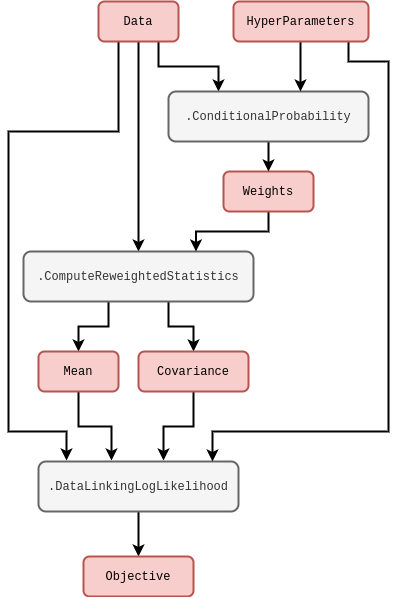
\includegraphics[width=8cm]{images/chapter-2-prob-reweighting-code.drawio.png}
\caption{Code schematic of the probability reweighting objective computation.}
\label{fig:prob-reweighting-code}
\end{figure} 

In order to specify what $P_{({\sf t}+1){\sf t}'}(x\vert x',z)$ is, it's quite natural to define a set of hyperparameters for the elements of $z$. To get a sense of how the data-linking function relates to these hyperparameters, it's instructive to consider an example. One generally-applicable option for the conditional probability could be a purely time-dependent kernel
%%
\begin{align}
P_{({\sf t}+1){\sf t}'}(x\vert x',z) &\propto {\cal K}(z, {\sf t}+1,{\sf t}')  \label{eq:time-dependent-kernel} \,, 
\end{align}
%%
and the data-linking distribution, e.g., could be a Gaussian
%%
\begin{align}
P_{{\sf t}+1}[y;M_{{\sf t}+1}(z),C_{{\sf t}+1}(z),\dots ] = {\sf MultivariateNormalPDF}[y;M_{{\sf t}+1}(z),C_{{\sf t}+1}(z)] \label{eq:gaussian-data-prob}\,.
\end{align}
%%
It's worth pointing out that other machine learning frameworks could easily be used to model these conditional probabilities. For example, neural networks could be used to infer the optimal reweighting scheme and this would still allow us to use the data-linking distribution.\footnote{One can think of using this neural network-based reweighting scheme as similar to constructing a normalising flow model~\cite{kobyzev2020normalizing} with an autoregressive layer. Invertibility and further network structural constraints mean that these are not exactly equivalent, however.} It would still be desirable to keep the data-linking distribution as it can usually be sampled from very easily --- something that can be quite difficult to achieve with a purely machine learning-based representation of the distribution. Sampling itself could even be made more flexible by leveraging a Variational Autoencoder (VAE)~\cite{pinheiro2021variational}; these use neural networks not just on the compression (or `encode') step to estimate the statistics but also use them as a layer between the sample from the data distribution model and the output (the `decode' step).

In the case of Eqs.~(\ref{eq:time-dependent-kernel}) and~(\ref{eq:gaussian-data-prob}) above, the hyperparameters that would be optimised could relate to the kernel in a wide variety of ways. Optimising them would make our optimised reweighting similar to (but very much \emph{not} the same as) evaluating maximum a posteriori (MAP) of a Gaussian process regression. In a Gaussian process regression, one is concerned with inferring the the whole of $X_{{\sf t}}$ as a function of time using the pairwise correlations implied by Eq.~(\ref{eq:second-order-log-expansion}). Based on this expression, the cumulative log-likelihood for a Gaussian process can be calculated as follows
%%
\begin{align}
\ln {\cal L}_{{\sf t}+1}(Y\vert z) &= -\frac{1}{2}\sum_{{\sf t}'=0}^{{\sf t}+1} \bigg[ n\ln (2\pi ) + \ln \big\vert {\cal H}_{({\sf t}+1){\sf t}'}(z)\big\vert + \sum_{i=0}^{n}\sum_{j=0}^{n} y^i {\cal H}^{ij}_{({\sf t}+1){\sf t}'}(z) (y')^j \bigg] \,. \label{eq:log-likelihood-gaussian-proc}    
\end{align}
%%

As we did for the reweighting algorithm, in Fig.~\ref{fig:gaussian-process-code} we have illustrated a schematic of the basic code needed to compute the objective function of a learning algorithm based on Eq.~(\ref{eq:log-likelihood-gaussian-proc}). Note that, in the expression above, we have replaced $x-x_*$ with $y$ and so it is assumed that the data has already been shifted such that its values are positioned around the distribution peak. Knowing where this peak will be a priori is not possible. However, for Gaussian data, an unbiased estimator for this peak will be the sample mean and so we have included an initial data standardisation in the steps outlined by Fig.~\ref{fig:gaussian-process-code}.

\begin{figure}[h]
\centering
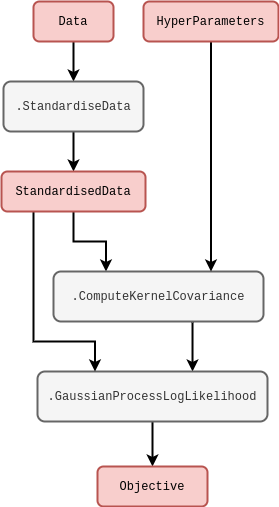
\includegraphics[width=6cm]{images/chapter-2-gaussian-process-code.drawio.png}
\caption{Code schematic of the Gaussian process objective computation.}
\label{fig:gaussian-process-code}
\end{figure}

The optimisation approach that we choose to use for obtaining the best hyperparameters in the conditional probability of Eq.~(\ref{eq:log-likelihood-reweighting}) will depend on a few factors. For example, if the number of hyperparameters is relatively low, but their gradients are difficult to calculate exactly; then a gradient-free optimiser (such as the Nelder-Mead~\cite{nelder1965simplex} method or something like a particle swarm~\cite{kennedy1995particle, shi1998modified}) would likely be the most effective choice. On the other hand, when the number of hyperparameters ends up being relatively large, it's usually quite desriable to utilise the gradients in algorithms like vanilla Stochastic Gradient Descent~\cite{robbins1951stochastic} (SGD) or Adam~\cite{kingma2014adam}.

If the gradients of Eq.~(\ref{eq:log-likelihood-reweighting}) are needed, we can always factorise each derivative with respect to hyperparameter $z^i$ in the following way through the chain rule
%%
\begin{align}
\frac{\partial}{\partial z^i}\ln {\cal L}_{{\sf t}+1}(Y \vert z) &= \sum_{{\sf t}'=0}^{{\sf t}+1}\frac{\partial M_{{\sf t}'}}{\partial z^i}\frac{\partial}{\partial M_{{\sf t}'}}\ln P_{{\sf t}'}[y;M_{{\sf t}'}(z),C_{{\sf t}'}(z),\dots ] \nonumber \\
&\qquad + \sum_{{\sf t}'=0}^{{\sf t}+1}\frac{\partial C_{{\sf t}'}}{\partial z^i}\frac{\partial }{\partial C_{{\sf t}'}}\ln P_{{\sf t}'}[y;M_{{\sf t}'}(z),C_{{\sf t}'}(z),\dots ] \,. \label{eq:log-likelihood-reweighting-grad}
\end{align}
%%
By factoring derivatives in this manner, the computation can be separated into two parts: the derivatives with respect to $M_{{\sf t}'}$ and $C_{{\sf t}'}$, which are typically quite straightforward; and the derivatives with respect to $z$ elements, which typically need a more involved calculation depending on the model. Incidentally, this separation also neatly lends itself to abstracting gradient calculations as having a simpler, general purpose component that can be built directly into a library of data models and a more complex, model-specific component that the user must specify.

The same logic should apply to a learning algorithm which optimises $z$ to obtain the MAP for a Gaussian process. If the gradients of Eq.~(\ref{eq:log-likelihood-gaussian-proc}) are required, the user would have to specify derivatives of the kernel matrix (and its determinant) with respect to $z$ in order to calculate
%%
\begin{align}
\frac{\partial}{\partial z^k}\ln {\cal L}_{{\sf t}+1}(Y \vert z) &= -\frac{1}{2}\sum_{{\sf t}'=0}^{{\sf t}+1} \bigg[ \frac{\partial}{\partial z^k}\ln \big\vert {\cal H}_{({\sf t}+1){\sf t}'}(z)\big\vert + \sum_{i=0}^{n}\sum_{j=0}^{n} y^i \frac{\partial}{\partial z^k}{\cal H}^{ij}_{({\sf t}+1){\sf t}'}(z) (y')^j \bigg] \,. \label{eq:log-likelihood-gaussian-proc-grad}
\end{align}
%%


    

\chapter{\sffamily Probabilistic online learning software}

{\bfseries\sffamily Concept.} To outline the software design characteristics of a probabilistic online learning framework, built to interface directly with our generalised simulation engine. The probabilistic algorithms we introduced in the previous chapter will form the basic set of tools in this framework. As well as its own implementations of useful algorithms, this software is also designed to make use of other machine learning APIs, e.g., Libtorch (via Gotch), and optimisation libraries, e.g., Gonum and eaopt. For the mathematically-inclined, this chapter will motivate online learning as an essential framework for our use case and how our probabilistic algorithms can work within this context. For the programmers, the software described in this chapter lives in the public Git repository: \href{https://github.com/umbralcalc/learnadex}{https://github.com/umbralcalc/learnadex}.

\textcolor{red}{Got to here in rewrite...}

\section{\sffamily Online learning with any algorithm}

Before discussing the software design aspects, we need to consider how we might structure learning by optimisation of Eq.~(\ref{eq:log-likelihood-reweighting}) for a sequence of observations in time. One of the issues that can arise when learning streams of data is `concept drift'. In our context, this would be when the optimal value for $z$ does not match the optimal value at some later point in time. In order to solve this issue, our learning algorithm should track an up-to-date optimal value for $z$ as data is continually passed into it. Iteratively updating the optimal parameters as new data is ingested into the objective function is typically called `online learning'~\cite{hazan2016introduction,sutton2018reinforcement}, in contrast to `offline learning' which would correspond to learning an optimal $z$ only once with the entire dataset provided upfront.\footnote{This book will mostly be focussed on using online learning techniques due to the inherently sequential nature of stochastic processes.}

\section{\sffamily Software design}

Let's now take a step back from the specifics of the probabilistic reweighting algorithm to introduce our new sofware package for this part of the book: the `learnadex'. At its core, the learnadex algorithm adapts the stochadex iteration engine to iterate through streams of data in order to accumulate a global objective function value with respect to that data. The user may then choose which optimisation algorithm (or write their own) to use in order to leverage this objective for learning a better representation of the data. 

As we discussed at the end of the last section, the algorithms in the learnadex are all applied in an `online' fashion --- refitting for the optimal hyperparameters $z$ as new data is streamed into them. A challenging aspect of online learning is in managing the computational expense of recomputing the optimal value for $z$ after each new datapoint is sent. To help with this; the user may configure the algorithm recompute the optimum value after larger batches of data have been ingested. The last value of optimum $z$ will also frequently be close to the next optimum in the sequence, so using the former as the initial input into the optimisation routine for the latter is typically very valuable for aiding efficiency.

Reusing the \texttt{PartitionCoordinator} code of the stochadex to facilitate online learning makes neat use of software which has already been designed and tested in earlier chapters of this book. However, in order to fully achieve this, a few minor extensions to the typing structures and code abstractions are necessary; as we show in Fig.~\ref{fig:learnadex-data-types-design}. To start with, we separate out `learning' from the kind of optimiser in the overall config so as to enable multiple optimisation algorithms to be used for the same learning problem. The hyperparameters that define that optimisation problem domain can be determined by the user with an extension to the \texttt{OtherParams} object so that it includes some optional Boolean masks over the parameters, i.e., \texttt{OtherParams.FloatParamMask} and \texttt{OtherParams.IntParamMask}. These masks are used to extract the parameters of interest, which can then be flattened and formatted to fit into any generic optimisation algorithm.

\begin{figure}[h]
\centering
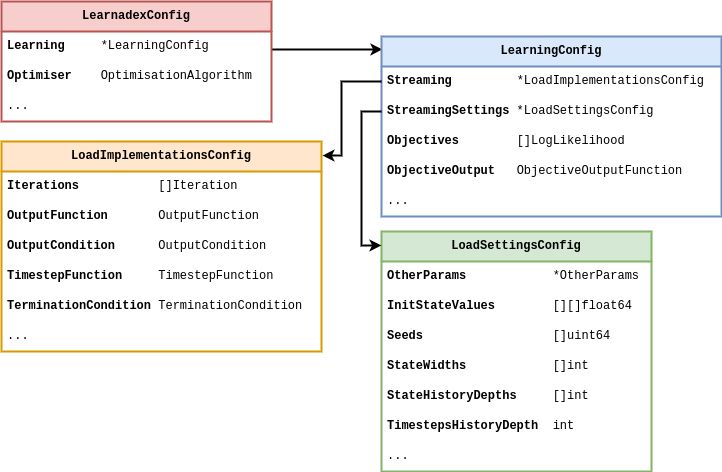
\includegraphics[width=12cm]{images/chapter-3-learnadex-data-types.drawio.png}
\caption{A relational summary of the core data types in the learnadex.}
\label{fig:learnadex-data-types-design}
\end{figure}

On the learning side; in order to define a specific objective for each data iterator to compute while the data streams through it, we have abstracted a `log-likelihood' type. Similarly, each iterator also gets a data streamer configuration which defines where the data is streaming from --- e.g., from a file on disk, from a local database instance or maybe via a network socket --- and also some inherited abstractions from the stochadex which define the time stepping function and when the data stream ends. In Fig.~\ref{fig:learnadex-data-iterator} below, we provide a schematic of the method calls of (and within) each data iterator.

\textcolor{red}{\begin{itemize}
\item{introduce the $\beta$ past discounting factor in this section and explain what it's for}
\item{refactor the code so that it's always doing online learning under the hood --- this can either be rolling refits in blocks on a refitting schedule with any optimisation algorithm of choice or full online learning Adam optimisation $$z_*({\sf t}+1) = -\alpha [{\sf t}+1,\text{stats of gradient history like Adam}] \frac{\partial}{\partial z} \ln {\cal L}_{{\sf t}+1} + z_*({\sf t})$$}
\item{refactor the code and integrate the reweighting algorithm with Libtorch models for the conditional probabilities --- describe how this is supported}
\item{describe the method calls diagram in more detail --- in particular, point out how it can replace the \texttt{Iteration.Iterate} method which is called when the \texttt{StateIterator} is asked for another iteration from the \texttt{PartitionCoordinator} of the stochadex}
\item{then talk about the optimiser! starting with non-gradient-based: the two packages that are supported out of the box are gonum and eaopt (still need to do gago --- see here: github.com/maxhalford/eaopt) }
\item{also need to then support gradient-based algorithms (like vanilla SGD) by implementing Eq.~(\ref{eq:log-likelihood-reweighting-grad}) for the current basic implementations in the learnadex --- shouldn't be too difficult!}
\item{then talk about the output - talk about the possibilities for output and what the default setting to json logs is for}
\item{could also be written to, e.g., a locally-hosted database server and the best-suited would be a NoSQL document database, e.g., MongoDB~\cite{mongodb}, but building something bespoke and simpler is more aligned with the use-case here and with the principles of this book}
\item{describe the need for log exploration and visualisation and then introduce logsplorer - a REST API for querying the json logs (with basic filtering and selection capabilities but could be extended to more advanced options) and optionally also launches a visualisation React app written in Typescript}
\item{note how this could be scaled to cloud services easily and remotely queried through the logsplorer API and visualised} 
\end{itemize}}

\begin{figure}[h]
\centering
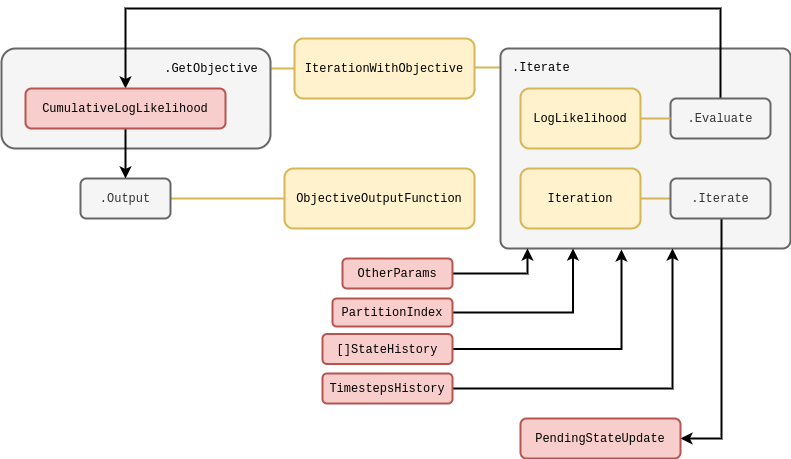
\includegraphics[width=14cm]{images/chapter-3-learnadex-data-iterator.drawio.png}
\caption{A schematic of an iteration with an objective function evaluation.}
\label{fig:learnadex-data-iterator}
\end{figure}

As with the software we wrote for the stochadex, the learnadex main binary executable leverages templating to enable full configurability of all the implementations and settings of Fig.~\ref{fig:learnadex-data-types-design} through passing configs at runtime. Users can alternatively use the learnadex as a library for import, if they desire more control over the code execution. 

\begin{figure}[h]
\centering
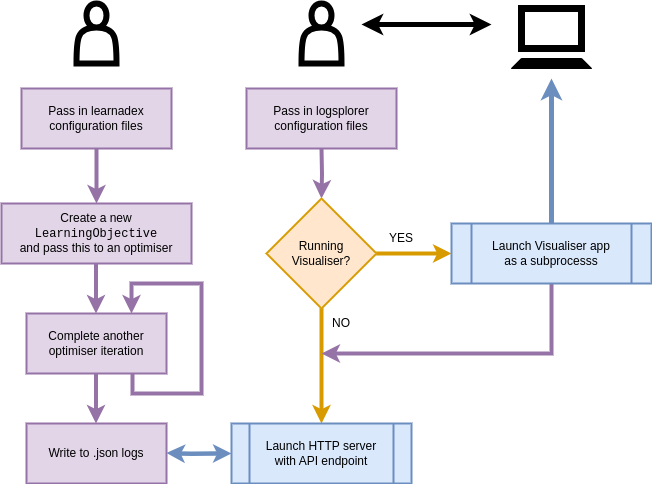
\includegraphics[width=13cm]{images/chapter-3-learnadex-main.drawio.png}
\caption{A diagram of the main learnadex and logsplorer executables.}
\label{fig:learnadex-main}
\end{figure}
    

\chapter{\sffamily Online simulation inference}

{\bfseries\sffamily Concept.} To extend the formalism that we developed in the previous chapter to describe the time evolution of state probabilities. Having introduced the basic concepts, we then use this formalism to motivate some important methods for probabilistic learning, which we then use in developing a framework for online simulation inference. For the mathematically-inclined, this chapter will take a detailed look at how our formalism can be extended to focus on the time evolution of probabilities, with a view to online simulation inference later on. For the programmers, all of the relevant software lives in this public Git repository: \href{https://github.com/umbralcalc/learndadex}{https://github.com/umbralcalc/learnadex}.

\section{\sffamily Probabilistic formalism} 

This book is about building more realistic training environments for machine learning systems in the real world. In the last chapter we formalised, designed and built a generalised simulation engine which could serve as the essential scaffolding for these environments. So why then, in this chapter, do we want to extend our formalism to talk about probabilistic learning methods?

For many of these realistic environments where only partial state observations are possible, probabilistic learning tools can immediately become an essential tool to robustly infer the state of a system and predict its future states from any given point in time. Given that these tools are often so important for extending the capability of learning algorithms to deal with partially-observed domains; we propose to extend the idea of what is more conventionally considered a `machine learning environment' to include tools for system state inference and future state prediction. In this sense, this chapter, and the remaining chapters of this book, will consider probabilistic learning as an essential part of the environment for a machine learning system.

In this chapter, we're going to begin by discussing the formal connections between some probabilistic learning methods and the simulation formalism we introduced in the last chapter. Let's start by returning to the formalism that we introduced in that chapter. As we discussed at that point; this formalism is appropriate for sampling from nearly every stochastic phenomenon that one can think of. We are going to extend this description to consider what happens to the probability that the state history matrix takes a particular set of values over time.

\begin{figure}[h]
\centering
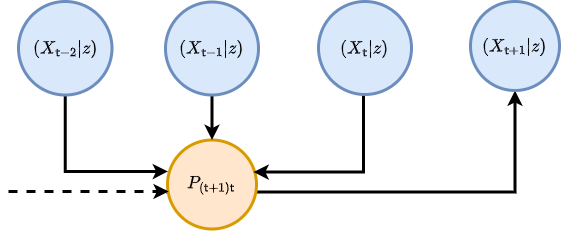
\includegraphics[width=12cm]{images/chapter-2-master-eq-graph.drawio.png}
\caption{Graph representation of Eq.~(\ref{eq:master-x-cont}).}
\label{fig:master-eqn}
\end{figure} 

So, how do we begin? Previously, we defined the general stochastic process with the formula $X^{i}_{{\sf t}+1} = F^{i}_{{\sf t}+1}(X_{0:{\sf t}},z,{\sf t})$. This equation also has an implicit \emph{master equation} associated to it that fully describes the time evolution of the \emph{probability density function} $P_{{\sf t}+1}(X\vert z)$ of $X_{0:{\sf t}+1}=X$ given that the parameters of the process are $z$. This can be written as
%%
\begin{align}
P_{{\sf t}+1}(X\vert z) &= P_{{\sf t}}(X'\vert z) P_{({\sf t}+1){\sf t}}(x\vert X',z) \label{eq:master-x-cont}\,,
\end{align}
%%
where for the time being we are assuming the state space is continuous in each of the matrix elements and $P_{({\sf t}+1){\sf t}}(x\vert X',z)$ is the conditional probability that $X_{{\sf t}+1}=x$ given that $X_{0:{\sf t}}=X'$ at time ${\sf t}$ and the parameters of the process are $z$. To try and understand what Eq.~(\ref{eq:master-x-cont}) is saying, we find it's helpful to think of an iterative relationship between probabilities; each of which is connected by their relative conditional probabilities. We've also illustrated this kind of thinking in Fig.~\ref{fig:master-eqn}.

Consider what happens when we extend the chain of conditional probabilities in Eq.~(\ref{eq:master-x-cont}) back in time by one step. In doing so, we retrieve a joint probability of rows $X_{{\sf t}+1}=x$ and $X_{{\sf t}}=x'$ on the right hand side of the expression 
%%
\begin{align}
P_{{\sf t}+1}(X\vert z) &= P_{{\sf t}-1}(X''\vert z) P_{({\sf t}+1){\sf t}({\sf t}-1)}(x,x'\vert X'',z) \label{eq:master-x-pairwise-joint}\,.
\end{align}
%%
Since Eqs.~(\ref{eq:master-x-cont}) and~(\ref{eq:master-x-pairwise-joint}) are both valid ways to obtain $P_{{\sf t}+1}(X\vert z)$ we can average between them without loss of generality in the original expression, like this
%%
\begin{align}
P_{{\sf t}+1}(X\vert z) &= \frac{1}{2}\big[ P_{{\sf t}}(X'\vert z) P_{({\sf t}+1){\sf t}}(x\vert X',z) + P_{{\sf t}-1}(X''\vert z) P_{({\sf t}+1){\sf t}({\sf t}-1)}(x,x'\vert X'',z) \big]\,.
\end{align}
%%
Following this line of reasoning to its natural conclusion, Eq.~(\ref{eq:master-x-cont}) can hence be generalised to consider all possible joint distributions of rows at different timesteps like this
%%
\begin{align}
P_{{\sf t}+1}(X\vert z) &= \frac{1}{{\sf t}}\sum_{{\sf t}''=0}^{{\sf t}}P_{{\sf t}''}(X''\vert z) P_{({\sf t}+1){\sf t}\dots{\sf t}''}(x,x',\dots \vert X'',z) \label{eq:master-x-cont-sum-gen}\,.
\end{align}
%%

If we wanted to just look at the distribution over the latest row $X_{{\sf t}+1}=x$, we could achieve this through marginalisation over all of the previous matrix rows in Eq.~(\ref{eq:master-x-cont}) like this
%%
\begin{align}
P_{{\sf t}+1}(x\vert z) = \int_{\Omega_{{\sf t}}}{\rm d}X' P_{{\sf t}+1}(X\vert z) &= \int_{\Omega_{{\sf t}}}{\rm d}X' P_{{\sf t}}(X'\vert z) P_{({\sf t}+1){\sf t}}(x\vert X',z) \label{eq:master-x-cont-latest-row} \,.
\end{align}
%%
But what is $\Omega_{\sf t}$? You can think of this as just the domain of possible matrix $X'$ inputs into the integral which will depend on the specific stochastic process we are looking at. 

The symbol ${\rm d}X'$ in Eq.~(\ref{eq:master-x-cont-latest-row}) is our shorthand notation throughout the book for computing the sum of integrals over previous state history matrices which can further be reduced via Eq.~(\ref{eq:master-x-cont-sum-gen}) into a product of sub-domain integrals over each matrix row
%%
\begin{align}
P_{{\sf t}+1}(x\vert z) &= \frac{1}{{\sf t}}\sum_{{\sf t}''=0}^{{\sf t}} \bigg\lbrace \int_{\omega_{{\sf t}'}}{\rm d}^nx'...\int_{\Omega_{{\sf t}''}}{\rm d}X'' \bigg\rbrace \,P_{{\sf t}''}(X''\vert z) P_{({\sf t}+1){\sf t}\dots{\sf t}''}(x,x',... \vert X'',z) \\
&= \frac{1}{{\sf t}}\sum_{{\sf t}''=0}^{{\sf t}} \int_{\Omega_{{\sf t}''}}{\rm d}X'' P_{{\sf t}''}(X''\vert z) P_{({\sf t}+1){\sf t}''}(x \vert X'',z) \label{eq:master-x-cont-latest-row-gen} \,,
\end{align}
%%
where each row measure is a Cartesian product of $n$ elements (a Lebesgue measure), i.e.,
%%
\begin{align}
{\rm d}^nx = \prod_{i=0}^n{\rm d}x^i \,,
\end{align}
%%
and lowercase $x, x', \dots$ values will always refer to individual rows within the state matrices. Note that $1/{\sf t}$ here is a normalisation factor --- this just normalises the sum of all probabilities to 1 given that there is a sum over ${\sf t}'$. Note also that, if the process is defined over continuous time, we would need to replace 
%%
\begin{align}
\frac{1}{{\sf t}}\sum_{{\sf t}'=0}^{{\sf t}} \rightarrow \frac{1}{t({\sf t})}\sum_{{\sf t}'=0}^{{\sf t}}\delta t({\sf t}') \,.
\end{align}
%%

Let's go through some examples. Non-Markovian phenomena with continuous state spaces can have quite complex master equations. A relatively simple example is that of pure diffusion processes which exhibit stochastic resetting at a rate $r$ to a remembered location from the trajectory history~\cite{boyer2017long}
%%
\begin{align}
P_{{\sf t}+1}(x\vert z) &= (1-r)P_{{\sf t}}(x\vert z) + \sum_{i=0}^n\sum_{j=0}^n\frac{\partial}{\partial x^i}\frac{\partial}{\partial x^j}\bigg[ D_{{\sf t}}(x,z)P_{{\sf t}}(x\vert z) \bigg] + r\sum_{{\sf t}'=0}^{{\sf t}}\delta t ({\sf t}')K[t({\sf t}){-}t({\sf t}')]P_{{\sf t}'}(x\vert z) \,,
\end{align}
%%
where here $K$ is some memory kernel. For Markovian phenomena which have a continuous state space, Eqs.~(\ref{eq:master-x-cont}) and~(\ref{eq:master-x-cont-latest-row}) no longer depend on timesteps older than the immediately previous one, hence, e.g., Eq.~(\ref{eq:master-x-cont-latest-row}) reduces to just
%%
\begin{align}
P_{{\sf t}+1}(x\vert z) &= \int_{\omega_{\sf t}}{\rm d}^nx' \, P_{\sf t}(x'\vert z) P_{({\sf t}+1){\sf t}}(x\vert x',z) \label{eq:master-x-cont-markov} \,.
\end{align}
%%
A famous example of this kind of phenomenon arises from approximating Eq.~(\ref{eq:master-x-cont-markov}) with an expansion (Kramers-Moyal~\cite{kramers1940brownian, moyal1949stochastic}) up to second-order, yielding the Fokker-Planck equation 
%%
\begin{align}
P_{{\sf t}+1}(x\vert z) &= P_{{\sf t}}(x\vert z) - \sum_{i=0}^n\frac{\partial}{\partial x^i}\bigg[ \mu_{{\sf t}}(x,z)P_{{\sf t}}(x\vert z)\bigg] + \sum_{i=0}^n\sum_{j=0}^n\frac{\partial}{\partial x^i}\frac{\partial}{\partial x^j}\bigg[ D_{{\sf t}}(x,z)P_{{\sf t}}(x\vert z) \bigg] \,,
\end{align}
%%
which describes a process undergoing drift-diffusion.

An analog of Eq.~(\ref{eq:master-x-cont-latest-row}) exists for discrete state spaces as well. We just need to replace the integral with a sum and the schematic would look something like this
%%
\begin{align}
P_{{\sf t}+1}(x\vert z) &= \sum_{\Omega_{{\sf t}}} P_{{\sf t}}(X'\vert z) P_{({\sf t}+1){\sf t}}(x \vert X', z) \label{eq:master-x-disc} \,,
\end{align}
%%
where we note that the $P$'s in the expression above all now refer to \emph{probability mass functions}. In what follows, discrete state space can always be considered by replacing the integrals with summations over probability masses in this manner; we only use the continuous state space formulation for our notation because one could argue it's a little more general. 

Analogously to continuous state spaces, we can give some examples of master equations for phenomena with a discrete state space as well. In the Markovian case, we need look no further than a simple time-dependent Poisson process
%%
\begin{align}
P_{{\sf t}+1}(x\vert z) &= \lambda ({\sf t}) \delta t({\sf t}{+}1)P_{{\sf t}}(x{-}1\vert z) + \big[1-\lambda ({\sf t}) \delta t({\sf t}{+}1)\big] P_{{\sf t}}(x\vert z) \,.
\end{align}
%%
For such an example of a non-Markovian system, a Hawkes process~\cite{hawkes1971spectra} master equation would look something like this
%%
\begin{align}
P_{{\sf t}+1}(x\vert z) &= \mu \delta t({\sf t}{+}1)P_{{\sf t}}(x{-}1\vert z) + \big[ 1-\mu \delta t({\sf t}{+}1)\big] P_{{\sf t}}(x\vert z) \nonumber \\
& + \sum_{x'=0}^\infty\sum_{{\sf t}'=0}^{{\sf t}} \phi [t({\sf t})-t({\sf t}')] \delta t({\sf t}{+}1)P_{{\sf t}{\sf t}'({\sf t}'-1)}(x{-}1,x',x'{-}1\vert z) \nonumber \\
&+ \sum_{x'=0}^\infty\bigg\lbrace 1-\sum_{{\sf t}'=0}^{{\sf t}} \phi [t({\sf t})-t({\sf t}')] \delta t({\sf t}{+}1)\bigg\rbrace P_{{\sf t}{\sf t}'({\sf t}'-1)}(x, x', x'{-}1\vert z) \,,
\end{align}
%%
where we note the complexity in this expression arises because it has to include a coupling between the rate at which events occur and an explicit memory of when the previous ones did occur (recorded by differencing the count between adjacent timesteps by 1).

\section{\sffamily Probabilistic learning algorithms}

So now that we are more familiar with the notation used by Eq.~(\ref{eq:master-x-cont-latest-row}), we can use it to motivate some useful probabilistic learning methods. While it's worth going into some mathematical detail to give a better sense of where each technique comes from, we should emphasise that the methodologies we discuss here are not new to the technical literature at all. We draw on influences from Empirical Dynamical Modeling (EDM)~\cite{sugihara1990nonlinear}, some classic nonparametric local regression techniques --- such as LOWESS/Savitzky-Golay filtering~\cite{savitzky1964smoothing} --- and also Gaussian processes~\cite{murphy2012machine}.  

Let's begin our discussion of algorithms by integrating Eq.~(\ref{eq:master-x-cont-latest-row}) over $x$ to obtain a relation for the mean of the distribution
%%
\begin{align}
M_{{\sf t}+1}(z) &= \int_{\omega_{{\sf t}+1}}{\rm d}^nx \,x\, P_{{\sf t}+1}(x\vert z) = \frac{1}{{\sf t}}\sum_{{\sf t}''=0}^{{\sf t}} \int_{\Omega_{{\sf t}''}}{\rm d}X'' P_{{\sf t}''}(X''\vert z) M_{({\sf t}+1){\sf t}''}(X'',z) \label{eq:mean-field-master}\,,
\end{align}
%%
where you can view the $M_{({\sf t}+1){\sf t}''}(X'',z)$ values as either terms in some regression model, or derivable explicitly from a known master equation. The latter of these provides one approach to statistically infer the states and parameters of stochastic simulations from data: one begins by knowing what the master equation is, uses this to compute the time evolution of the mean (and potentially higher-order statistics) and then connects these ${\sf t}$ and $z$-dependent statistics back to the likelihood of observing the data. This is what is commonly known as the `mean-field' inference approach; averaging over the available degrees of freedom in the statistical moments of distributions. Though, knowing what the master equation is for an arbitrarily-defined stochastic phenomenon can be very difficult indeed, and the resulting equations typically require some form of approximation. 

\begin{figure}[h]
\centering
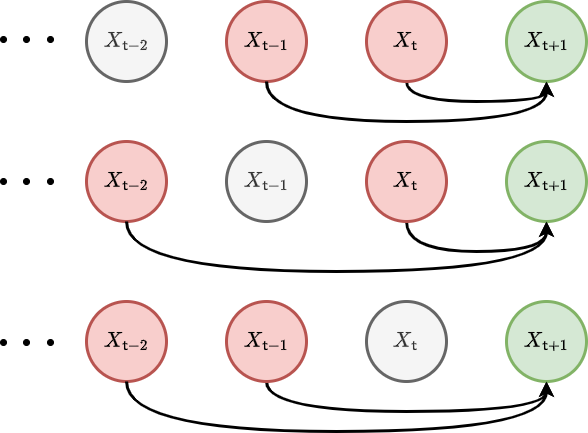
\includegraphics[width=8cm]{images/chapter-2-second-temporal-correlation.drawio.png}
\caption{A graph representation of the correlations in Eq.~(\ref{eq:second-order-correl}).}
\label{fig:second-temporal-correlation}
\end{figure} 

Given that the mean-field approach isn't always going to be viable as an inference method, we should also consider other ways to describe the shape and time evolution characteristics of $P_{{\sf t}+1}(X\vert z)$. For continuous state spaces, it's possible to approximate this whole distribution with a logarithmic expansion like so
%%
\begin{align}
\ln P_{{\sf t}+1}(X\vert z) &\simeq \ln P_{{\sf t}+1}(X_*\vert z) + \frac{1}{2}\sum_{{\sf t}'=0}^{{\sf t}+1}\sum_{i=0}^{n}\sum_{j=0}^{n} (x-x_*)^i {\cal H}^{ij}_{({\sf t}+1){\sf t}'}(z) (x'-x'_*)^j \label{eq:second-order-log-expansion} \\
{\cal H}^{ij}_{({\sf t}+1){\sf t}'}(z) &= \frac{\partial}{\partial x^i}\frac{\partial}{\partial (x')^j}\ln P_{{\sf t}+1}(X\vert z) \bigg\vert_{X=X_*} \label{eq:second-order-log-expansion-kernel} \,,
\end{align}
%% 
where the values for $X_*$ (and its rows $x_*, x_*', \dots$) are defined by the vanishing of the first derivative, i.e., these are chosen such that
%%
\begin{align}
\frac{\partial}{\partial x^i}\ln P_{{\sf t}+1}(X\vert z) \bigg\vert_{X=X_*} &= 0 \,.
\end{align}
%%
This logarithmic expansion is one way to see how a Gaussian process regression is able to approximate $X_{{\sf t}}$ evolving in time for many different processes. By selecting the appropriate function for the kernel given by Eq.~(\ref{eq:second-order-log-expansion-kernel}), a Gaussian process regression can be fully specified.

If we keep the truncation up to second order in Eq.~(\ref{eq:second-order-log-expansion}), note that this expression implies a pairwise correlation structure of the form
%%
\begin{align}
P_{{\sf t}+1}(X\vert z) &\rightarrow \prod_{{\sf t}'=0}^{{\sf t}}P_{({\sf t}+1){\sf t}'}(x,x'\vert z) = \prod_{{\sf t}'=0}^{{\sf t}}P_{{\sf t}'}(x'\vert z)P_{({\sf t}+1){\sf t}'}(x\vert x', z) \,.
\end{align}
%%
Given this pairwise temporal correlation structure, Eq.~(\ref{eq:master-x-cont-latest-row-gen}) reduces to this simpler sum of integrals
%%
\begin{align}
P_{{\sf t}+1}(x\vert z) &= \frac{1}{{\sf t}}\sum_{{\sf t}'=0}^{{\sf t}}\int_{\omega_{{\sf t}'}}{\rm d}^nx' P_{{\sf t}'}(x'\vert z)P_{({\sf t}+1){\sf t}'}(x\vert x',z) \label{eq:second-order-correl} \,.
\end{align}
%%
We have illustrated these second-order correlations with a graph visualisation in Fig.~(\ref{fig:second-temporal-correlation}).

\begin{figure}[h]
\centering
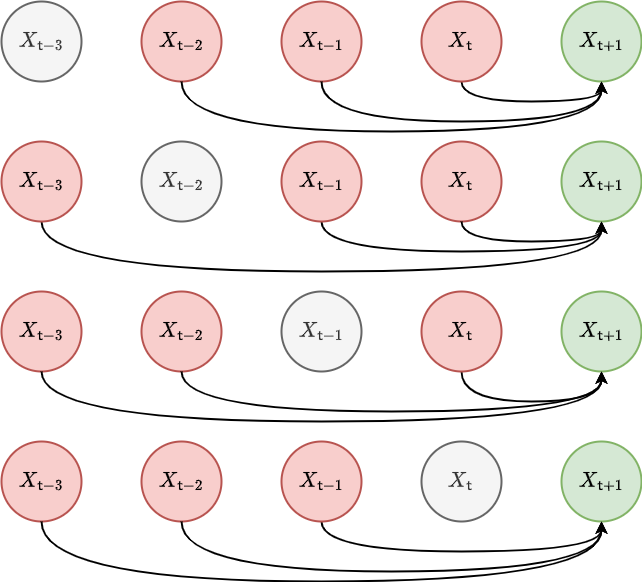
\includegraphics[width=10cm]{images/chapter-2-third-temporal-correlation.drawio.png}
\caption{A graph representation of the correlations in Eq.~(\ref{eq:third-order-correl}).}
\label{fig:third-temporal-correlation}
\end{figure}

In a similar fashion, we can increase the expansion order of Eq.~(\ref{eq:second-order-log-expansion}) to include third-order correlations such that 
%%
\begin{align}
P_{{\sf t}+1}(X\vert z) &\rightarrow \prod_{{\sf t}'=0}^{{\sf t}}\prod_{{\sf t}''=0}^{{\sf t}'-1} P_{{\sf t}'{\sf t}''}(x',x''\vert z)P_{({\sf t}+1){\sf t}'{\sf t}''}(x\vert x',x'',z) \,,
\end{align}
%%
and, in this instance, one can show that Eq.~(\ref{eq:master-x-cont-latest-row-gen}) reduces to
%%
\begin{align}
P_{{\sf t}+1}(x\vert z) &= \frac{1}{{\sf t}}\sum_{{\sf t}'=0}^{{\sf t}}\frac{1}{{\sf t}'-1}\sum_{{\sf t}''=0}^{{\sf t}'-1}\int_{\omega_{{\sf t}'}}{\rm d}^nx'\int_{\omega_{{\sf t}''}}{\rm d}^nx'' P_{{\sf t}'{\sf t}''}(x',x''\vert z)P_{({\sf t}+1){\sf t}'{\sf t}''}(x\vert x',x'',z) \label{eq:third-order-correl} \,.
\end{align}
%%
We have also illustrated these third-order correlations with another graph visualisation in Fig.~(\ref{fig:third-temporal-correlation}). Using $P_{{\sf t}'{\sf t}''}(x',x''\vert z) = P_{{\sf t}''}(x''\vert z) P_{{\sf t}'{\sf t}''}(x'\vert x'', z)$ one can also show that this integral is a marginalisation of this expression
%%
\begin{align}
P_{({\sf t}+1){\sf t}''}(x\vert x'', z) &= \frac{1}{{\sf t}}\sum_{{\sf t}'=0}^{{\sf t}}\int_{\omega_{{\sf t}'}}{\rm d}^nx'P_{{\sf t}'{\sf t}''}(x'\vert x'',z)P_{({\sf t}+1){\sf t}'{\sf t}''}(x\vert x',x'',z) \,,
\end{align}
%%
which describes the time evolution of the conditional probabilities. Note how this implies that the Gaussian process kernel itself can be evolved through time to replicate these higher-order temporal correlations for a regression problem, if desired.

Another probabilistic learning algorithm that we can consider is what we shall call `empirical probabilistic reweighting'. There is another expression for the mean of the distribution, that we can derive under certain conditions, which will be valuable to motivating this algorithm. If the probability distribution over each row of the state history matrix is \emph{stationary} --- meaning that $P_{{\sf t}+1}(x\vert z)=P_{{\sf t}'}(x\vert z)$ --- it's possible to go one step further than Eq.~(\ref{eq:mean-field-master}) and assert that
%%
\begin{align}
M_{{\sf t}+1}(z) &= \int_{\omega_{{\sf t}+1}}{\rm d}^nx \,x\,P_{{\sf t}+1}(x\vert z) = \frac{1}{{\sf t}}\sum_{{\sf t}'=0}^{{\sf t}}\int_{\omega_{{\sf t}'}}{\rm d}^nx' \,x'\, P_{{\sf t}'}(x'\vert z) \int_{\omega_{{\sf t}+1}}{\rm d}^nx\, P_{({\sf t}+1){\sf t}'}(x\vert x',z) \label{eq:stationary-mean-estimator}\,.
\end{align}
%%

To see that Eq.~(\ref{eq:stationary-mean-estimator}) is true, first note that a joint distribution over both $x$ and $x'$ can be derived like this $P_{({\sf t}+1){\sf t}'}(x,x'\vert z)=P_{({\sf t}+1){\sf t}'}(x\vert x',z)P_{{\sf t}'}(x'\vert z)$. Secondly, note that this joint distribution will always allow variable swaps trivially like this $P_{({\sf t}+1){\sf t}'}(x,x'\vert z)=P_{{\sf t}'({\sf t}+1)}(x',x\vert z)$. Then, lastly, note that stationarity of $P_{{\sf t}+1}(x\vert z)=P_{{\sf t}'}(x\vert z)$ means 
%%
\begin{align}
\frac{1}{{\sf t}}\sum_{{\sf t}'=0}^{{\sf t}}\int_{\omega_{{\sf t}+1}} {\rm d}^nx\int_{\omega_{{\sf t}'}} {\rm d}^nx' \,x\, P_{({\sf t}+1){\sf t}'}(x,x'\vert z)&=\frac{1}{{\sf t}}\sum_{{\sf t}'=0}^{{\sf t}}\int_{\omega_{{\sf t}'}} {\rm d}^nx\int_{\omega_{{\sf t}+1}} {\rm d}^nx' \,x\, P_{{\sf t}'({\sf t}+1)}(x,x'\vert z)\nonumber \\
&=\frac{1}{{\sf t}}\sum_{{\sf t}'=0}^{{\sf t}}\int_{\omega_{{\sf t}'}} {\rm d}^nx'\int_{\omega_{{\sf t}+1}} {\rm d}^nx \,x'\, P_{({\sf t}+1){\sf t}'}(x,x'\vert z) \nonumber \\
&=\frac{1}{{\sf t}}\sum_{{\sf t}'=0}^{{\sf t}}\int_{\omega_{{\sf t}'}}{\rm d}^nx' \,x'\, P_{{\sf t}'}(x'\vert z) \int_{\omega_{{\sf t}+1}}{\rm d}^nx\, P_{({\sf t}+1){\sf t}'}(x\vert x',z)\nonumber \,,
\end{align}
%%
where we've used the trivial variable swap and integration variable relabelling to arrive at the second equality in the expressions above. 

The standard covariance matrix elements can also be computed in a similar fashion
%%
\begin{align}
C^{ij}_{{\sf t}+1}(z) &= \int_{\omega_{{\sf t}+1}}{\rm d}^nx \,[x-M_{{\sf t}+1}(z)
]^i[x-M_{{\sf t}+1}(z)]^jP_{{\sf t}+1}(x\vert z) \nonumber \\
&= \frac{1}{{\sf t}}\sum_{{\sf t}'=0}^{{\sf t}}\int_{\omega_{{\sf t}'}}{\rm d}^nx' \, [x'-M_{{\sf t}+1}(z)]^i[x'-M_{{\sf t}+1}(z)]^j \,P_{{\sf t}'}(x'\vert z) \int_{\omega_{{\sf t}+1}}{\rm d}^nx \, P_{({\sf t}+1){\sf t}'}(x\vert x',z) \label{eq:stationary-covariance-estimator}\,.
\end{align}
%%
While they look quite abstract, Eqs.~(\ref{eq:stationary-mean-estimator}) and~(\ref{eq:stationary-covariance-estimator}) express the core idea behind how the probabilistic reweighting will function. By assuming a stationary distribution, we gain the ability to directly estimate the statistics of the probability distribution of the next sample from the stochastic process $P_{{\sf t}+1}(x\vert z)$ from past samples it may have in empirical data; which are represented here by $P_{{\sf t}'}(x'\vert z)$.

Probabilistic reweighting depends on the stationarity of $P_{{\sf t}+1}(x\vert z)=P_{{\sf t}'}(x\vert z)$ such that, e.g., Eq.~(\ref{eq:stationary-mean-estimator}) is applicable. The core idea behind it is to represent the past distribution of state values $P_{{\sf t}'}(x'\vert z)$ with the samples from a real time series dataset. If the user then specifies a good model for the relationships in this data by providing a weighting function which returns the conditional probability mass
%%
\begin{align}
{\sf w}_{{\sf t}'}(y,z) = \int_{\omega_{{\sf t}+1}} {\rm d}^nx \, P_{({\sf t}+1){\sf t}'}(x\vert x'{=}y,z) \,,  
\end{align}
%%
we can apply this as a \emph{reweighting} of the historical time series samples to estimate any statistics of interest. Taking Eqs.~(\ref{eq:stationary-mean-estimator}) and~(\ref{eq:stationary-covariance-estimator}) as the examples; we are essentially approximating these integrals through weighted sample estimations like this
%%
\begin{align}
M_{{\sf t}+1}(z) &\simeq \frac{1}{{\sf t}}\sum^{{\sf t}}_{{\sf t}'=0}Y_{{\sf t}'} {\sf w}_{{\sf t}'}(Y_{{\sf t}'},z) \label{eq:mean-reweighting} \\
C^{ij}_{{\sf t}+1}(z) &\simeq \frac{1}{{\sf t}}\sum^{{\sf t}}_{{\sf t}'=0}[Y_{{\sf t}'}-M_{{\sf t}+1}(z)]^i[Y_{{\sf t}'}-M_{{\sf t}+1}(z)]^j \, {\sf w}_{{\sf t}'}(Y_{{\sf t}'},z) \label{eq:covariance-reweighting} \,,
\end{align}
%%
where we have defined the data matrix $Y$ with rows $Y_{{\sf t}+1}, Y_{{\sf t}}, \dots$, each of which representing specific observations of the rows in $X$ at each point in time from a real dataset.

The goal of a learning algorithm for probabilistic reweighting would be to learn the optimal reweighting function ${\sf w}_{{\sf t}'}(Y_{{\sf t}'},z)$ with respect to $z$, i.e., the ones which most accurately represent a provided dataset. But before we think about the various kinds of conditional probability we could use, we need to think about how to connect the post-reweighting statistics to the data by defining an objective function. 

If the mean is a sufficient statistic for the distribution which describes the data, a choice of, e.g., Exponential, Poisson or Binomial distribution could be used where the mean is estimated directly from the time series using Eq.~(\ref{eq:stationary-mean-estimator}), given a conditional probability $P_{({\sf t}+1){\sf t}'}(x\vert x',z)$. Extending this idea further to include distributions which also require a variance to be known, e.g., the Normal, Gamma or Negative Binomial distributions could be used where the variance (and/or covariance) could be estimated using Eq.~(\ref{eq:stationary-covariance-estimator}). These are just a few simple examples of distributions that can link the estimated statistics from Eqs.~(\ref{eq:stationary-mean-estimator}) and~(\ref{eq:stationary-covariance-estimator}) to a time series dataset. However, the algorithmic framework is very general to whatever choice of `data linking' distribution that a researcher might need.

We should probably make what we've just said a little more mathematically concrete. We can define $P_{{\sf t}+1}[y;M_{{\sf t}+1}(z),C_{{\sf t}+1}(z),\dots ]$ as representing the likelihood of $y = Y_{{\sf t}+1}$ given the estimated statistics from Eqs.~(\ref{eq:stationary-mean-estimator}) and~(\ref{eq:stationary-covariance-estimator}) (and maybe higher-orders). Note that in order to do this, we need to identify the $x'$ and ${\sf t}'$ values that are used to estimate, e.g., $M_{{\sf t}+1}(z)$ with the past data values which are observed in the dataset time series itself. Now that we have this likelihood, we can immediately evaluate an objective function (a cumulative log-likelihood) that we might seek to optimise over for a given dataset 
%%
\begin{align}
\ln {\cal L}_{{\sf t}+1}(Y\vert z) &= \sum_{{\sf t}'=0}^{{\sf t}+1} \ln P_{{\sf t}'}[y;M_{{\sf t}'}(z),C_{{\sf t}'}(z),\dots ] \,, \label{eq:log-likelihood-reweighting}
\end{align}
%%
where the summation continues until all of the past measurements $Y_{{\sf t}+1}, Y_{{\sf t}}, \dots$ which exist as rows in the data matrix $Y$ have been taken into account. The code to compute this objective function follows the schematic we have provided in Fig.~\ref{fig:prob-reweighting-code}.

\begin{figure}[h]
\centering
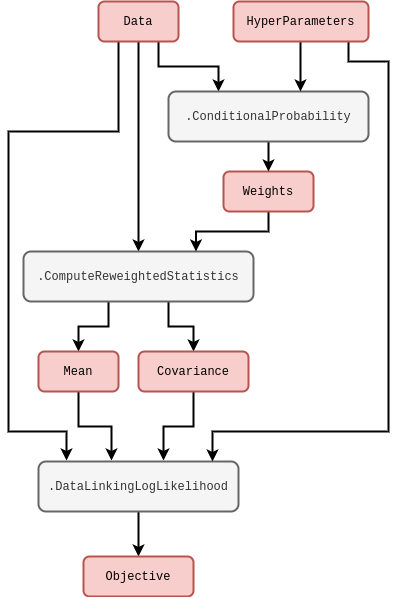
\includegraphics[width=8cm]{images/chapter-2-prob-reweighting-code.drawio.png}
\caption{Code schematic of the probability reweighting objective computation.}
\label{fig:prob-reweighting-code}
\end{figure} 

In order to specify what $P_{({\sf t}+1){\sf t}'}(x\vert x',z)$ is, it's quite natural to define a set of hyperparameters for the elements of $z$. To get a sense of how the data-linking function relates to these hyperparameters, it's instructive to consider an example. One generally-applicable option for the conditional probability could be a purely time-dependent kernel
%%
\begin{align}
P_{({\sf t}+1){\sf t}'}(x\vert x',z) &\propto {\cal K}(z, {\sf t}+1,{\sf t}')  \label{eq:time-dependent-kernel} \,, 
\end{align}
%%
and the data-linking distribution, e.g., could be a Gaussian
%%
\begin{align}
P_{{\sf t}+1}[y;M_{{\sf t}+1}(z),C_{{\sf t}+1}(z),\dots ] = {\sf MultivariateNormalPDF}[y;M_{{\sf t}+1}(z),C_{{\sf t}+1}(z)] \label{eq:gaussian-data-prob}\,.
\end{align}
%%
It's worth pointing out that other machine learning frameworks could easily be used to model these conditional probabilities. For example, neural networks could be used to infer the optimal reweighting scheme and this would still allow us to use the data-linking distribution.\footnote{One can think of using this neural network-based reweighting scheme as similar to constructing a normalising flow model~\cite{kobyzev2020normalizing} with an autoregressive layer. Invertibility and further network structural constraints mean that these are not exactly equivalent, however.} It would still be desirable to keep the data-linking distribution as it can usually be sampled from very easily --- something that can be quite difficult to achieve with a purely machine learning-based representation of the distribution. Sampling itself could even be made more flexible by leveraging a Variational Autoencoder (VAE)~\cite{pinheiro2021variational}; these use neural networks not just on the compression (or `encode') step to estimate the statistics but also use them as a layer between the sample from the data distribution model and the output (the `decode' step).

In the case of Eqs.~(\ref{eq:time-dependent-kernel}) and~(\ref{eq:gaussian-data-prob}) above, the hyperparameters that would be optimised could relate to the kernel in a wide variety of ways. Optimising them would make our optimised reweighting similar to (but very much \emph{not} the same as) evaluating maximum a posteriori (MAP) of a Gaussian process regression. In a Gaussian process regression, one is concerned with inferring the the whole of $X_{{\sf t}}$ as a function of time using the pairwise correlations implied by Eq.~(\ref{eq:second-order-log-expansion}). Based on this expression, the cumulative log-likelihood for a Gaussian process can be calculated as follows
%%
\begin{align}
\ln {\cal L}_{{\sf t}+1}(Y\vert z) &= -\frac{1}{2}\sum_{{\sf t}'=0}^{{\sf t}+1}\sum_{{\sf t}''=0}^{{\sf t}'} \bigg[ n\ln (2\pi ) + \ln \big\vert {\cal H}_{{\sf t}'{\sf t}''}(z)\big\vert + \sum_{i=0}^{n}\sum_{j=0}^{n} Y^i_{{\sf t}'} {\cal H}^{ij}_{{\sf t}'{\sf t}''}(z) Y^j_{{\sf t}''} \bigg] \,. \label{eq:log-likelihood-gaussian-proc}    
\end{align}
%%

As we did for the reweighting algorithm, in Fig.~\ref{fig:gaussian-process-code} we have illustrated a schematic of the basic code needed to compute the objective function of a learning algorithm based on Eq.~(\ref{eq:log-likelihood-gaussian-proc}). Note that, in the expression above, we have assumed that the data has already been shifted such that its values are positioned around the distribution peak. Knowing where this peak will be a priori is not possible. However, for Gaussian data, an unbiased estimator for this peak will be the sample mean and so we have included an initial data standardisation in the steps outlined by Fig.~\ref{fig:gaussian-process-code}.

\begin{figure}[h]
\centering
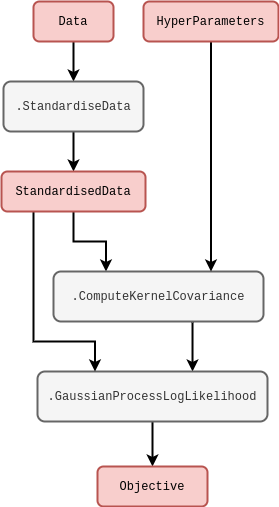
\includegraphics[width=6cm]{images/chapter-2-gaussian-process-code.drawio.png}
\caption{Code schematic of the Gaussian process objective computation.}
\label{fig:gaussian-process-code}
\end{figure}

The optimisation approach that we choose to use for obtaining the best hyperparameters in the conditional probability of Eq.~(\ref{eq:log-likelihood-reweighting}) will depend on a few factors. For example, if the number of hyperparameters is relatively low, but their gradients are difficult to calculate exactly; then a gradient-free optimiser (such as the Nelder-Mead~\cite{nelder1965simplex} method or something like a particle swarm~\cite{kennedy1995particle, shi1998modified}) would likely be the most effective choice. On the other hand, when the number of hyperparameters ends up being relatively large, it's usually quite desriable to utilise the gradients in algorithms like vanilla Stochastic Gradient Descent~\cite{robbins1951stochastic} (SGD) or Adam~\cite{kingma2014adam}.

If the gradients of Eq.~(\ref{eq:log-likelihood-reweighting}) are needed, we can always factorise each derivative with respect to hyperparameter $z^i$ in the following way through the chain rule
%%
\begin{align}
\frac{\partial}{\partial z^i}\ln {\cal L}_{{\sf t}+1}(Y \vert z) &= \sum_{{\sf t}'=0}^{{\sf t}+1}\frac{\partial M_{{\sf t}'}}{\partial z^i}\frac{\partial}{\partial M_{{\sf t}'}}\ln P_{{\sf t}'}[y;M_{{\sf t}'}(z),C_{{\sf t}'}(z),\dots ] \nonumber \\
&\qquad + \sum_{{\sf t}'=0}^{{\sf t}+1}\frac{\partial C_{{\sf t}'}}{\partial z^i}\frac{\partial }{\partial C_{{\sf t}'}}\ln P_{{\sf t}'}[y;M_{{\sf t}'}(z),C_{{\sf t}'}(z),\dots ] \,. \label{eq:log-likelihood-reweighting-grad}
\end{align}
%%
By factoring derivatives in this manner, the computation can be separated into two parts: the derivatives with respect to $M_{{\sf t}'}$ and $C_{{\sf t}'}$, which are typically quite straightforward; and the derivatives with respect to $z$ elements, which typically need a more involved calculation depending on the model. Incidentally, this separation also neatly lends itself to abstracting gradient calculations as having a simpler, general purpose component that can be built directly into a library of data models and a more complex, model-specific component that the user must specify.

The same logic should apply to a learning algorithm which optimises $z$ to obtain the MAP for a Gaussian process. If the gradients of Eq.~(\ref{eq:log-likelihood-gaussian-proc}) are required, the user would have to specify derivatives of the kernel matrix (and its determinant) with respect to each hyperparameter $z^k$ in order to calculate
%%
\begin{align}
\frac{\partial}{\partial z^k}\ln {\cal L}_{{\sf t}+1}(Y \vert z) &= -\frac{1}{2}\sum_{{\sf t}'=0}^{{\sf t}+1}\sum_{{\sf t}''=0}^{{\sf t}'} \bigg[ \frac{\partial}{\partial z^k}\ln \big\vert {\cal H}_{{\sf t}'{\sf t}''}(z)\big\vert + \sum_{i=0}^{n}\sum_{j=0}^{n} Y^i_{{\sf t}'} \frac{\partial}{\partial z^k}{\cal H}^{ij}_{{\sf t}'{\sf t}''}(z)Y^j_{{\sf t}''} \bigg] \,. \label{eq:log-likelihood-gaussian-proc-grad}
\end{align}
%%

\section{\sffamily Online learning with any algorithm}

We have discussed the importance of probabilistic learning in the context of environments where only partial state observability is possible and, in the previous chapter, we motivated the use of some specific probabilistic learning methods. However, we haven't yet discussed how we might implement a learning algorithm in practice. In particular, before covering the various aspects of software design, it's important to consider how we want to structure learning by optimisation of an objective with respect to a stream of time series data.

One of the issues that can arise when learning streams of data is `concept drift'. In our context, this would be when the optimal value for $z$ does not match the optimal value at some later point in time. In order to mitigate this, our learning algorithms should be able to track an up-to-date optimal value for $z$ as data is continually passed into them. Iteratively updating the optimal parameters as new data is ingested into the objective function is typically called `online learning'~\cite{hazan2016introduction,sutton2018reinforcement}, in contrast to `offline learning' which would correspond to learning an optimal $z$ only once with the entire dataset provided upfront.

The reader may recall that this book is about building more realistic environments for machine learning systems. An important part of learning from environments in a robust manner is ensuring \emph{adaptability to new data}. In addition to this, stochastic processes are inherently sequential. Many types of system evolve not just their states, but also dynamical description, over time. Online learning is the natural framework to use in this context.

Let's return to the models we discussed in the previous chapter which optimise the cumulative log-likelihood of the data matrix $Y$ with respect to $z$ at a particular point in time, i.e., which optimise $\ln {\cal L}_{{\sf t}+1}(Y\vert z)$ with respect to $z$ at time ${\sf t}+1$. The simplest (and most generally applicable) way to implement an online learning approach with any machine learning model is to rerun the whole optimisation algorithm for $z$ after each new datapoint $y$ has been received. Each time the optimisation is rerun, it will be using the entire batch of training data --- here represented by the data matrix $Y$. This kind of `batch' online learning will work for most of the standard machine learning algorithms, but the re-training process can take a long time to run in each instance. 

One way to speed things up is to assume that the optimal value for $z$ which was obtained from the previous data iterations is close to the one we will find in the most recent iteration. Hence, by inserting this previous value into the next run of the optimisation procedure as an initial guess, the algorithm will typically converge much more quickly to the optimum. This is more of a practical insight, but are there any quantitative methods which can reduce the amount of computation required to update $z$ when the latest datapoint in the series has been received?

This is where `pure' online learning comes in. When gradients of the log-likelihood are available, we can make things much more efficient. Consider ${\cal L}_{{\sf t}+1}(y\vert z)$ as the log-likelihood term for datapoint $y$ such that the cumulative log-likelihood of the data matrix $Y$ can be written as the following summation of terms
%%
\begin{align}
\ln {\cal L}_{{\sf t}+1}(Y\vert z) = \sum^{{\sf t}+1}_{{\sf t}'=0}\ln {\cal L}_{{\sf t}'}(y\vert z)\,.
\end{align}
%%
If we now denote the $z$ which we have learned from the data up to timestep ${\sf t}$ as $z_*({\sf t})$, we may write the following expression which uses the gradient of the log-likelihood to learn from each new datapoint arrival
%%
\begin{align}
z^i_*({\sf t}+1) &= z^i_*({\sf t}) - \alpha ({\sf t}+1,\dots ) \frac{\partial}{\partial z^i} \ln {\cal L}_{{\sf t}+1}(y\vert z) \label{eq:sgd-online} \,,
\end{align}
%%
which is based on a stochastic gradient descent (SGD) algorithm approach. In contrast to the more standard offline SGD approach --- which would be applied to mini-batches of the data --- this update is applied to $z_*$ using the log-likelihood at each point in time in sequence.

In Eq.~(\ref{eq:sgd-online}) the $\alpha ({\sf t}+1,\dots )$ function, or `learning rate' function, returns a value which controls the step size towards the optimal value. As indicated by the arguments to this function, the learning rate can be time-dependent, which allows the user to set a schedule of steps which help convergence in certain problems. Other inputs can depend on the specific flavour of stochastic gradient descent algorithm that is being run. For example, an Adam optimiser~\cite{kingma2014adam} makes use of the statistics computed from the history of gradient values obtained as the algorithm progresses.

\textcolor{red}{Still need to discuss:
\begin{itemize}
\item{batch learning algorithms --- more like Gaussian processes}
\item{`pure' online learning algorithms --- more like empirical probabilistic reweighting}
\end{itemize}}

\textcolor{red}{Got to here in rewrite...}

Note that other excellent online machine learning frameworks are available --- see, e.g., River~\cite{river} and Vowpal Wabbit~\cite{vowpalwabbit}. The motivation for designing our own probabilistic online learning software is to ensure maximal integration with the stochadex simulation engine. We'll aim to achieve this by designing the code to use the same data structures and and concepts as we used when building the stochadex, where possible. In the next section on software design, we will show how this can be done while still maintaining extensibility and interoperability with other machine learning libraries and APIs. So let's get on with it!

\section{\sffamily Simulation inference formalism}

In Bayesian inference, one applies Bayes' rule to the problem of statistically inferring a model from some dataset. This typically involves the following formula for a posterior distribution
%%
\begin{align}
{\cal P}_{{\sf t}+1}(z \vert Y) \propto {\cal L}_{{\sf t}+1}(Y\vert z){\cal P} (z) \label{eq:bayes-rule} \,.
\end{align}
%%
In the formula above, one relates the prior probability distribution over a parameter set ${\cal P} (z)$ and the likelihood ${\cal L}_{{\sf t}+1}(Y\vert z)$  of some data matrix $Y$ up to timestep ${\sf t}+1$ given the parameters $z$ of a model to the posterior probability distribution of parameters given the data ${\cal P}_{{\sf t}+1}(z \vert Y)$ up to some proportionality constant. All this may sound a bit technical in statistical language, so it can also be helpful to summarise what the formula above states verbally as follows: the initial (prior) state of knowledge about the parameters $z$ we want to learn can be updated by some likelihood function of the data to give a new state of knowledge about the values for $z$ (the `posterior' probability). 

From the point of view of statistical inference, if we seek to maximise ${\cal P}_{{\sf t}+1}(z \vert Y)$ --- or its logarithm --- in Eq.~(\ref{eq:bayes-rule}) with respect to $z$, we will obtain what is known as a maximum posteriori (MAP) estimate of the parameters. In fact, we have already encountered this metholodology in the previous chapter when discussing the algorithm which obtains the best fit parameters for the empirical probability reweighting. In this case; while it appears that we optimised the log-likelihood directly as our objective function, one can easily show that this is also technically equivalent obtaining a MAP estimate where one chooses a specfic prior ${\cal P} (z) \propto 1$ (typically known as a `flat prior').

How might we calulate the posterior in practice with some arbitrary stochastic process model that has been defined in the stochadex? In order to make the comparison to a real dataset, any stochadex model of interest will always need to be able to generate observations which can be directly compared to the data. To formalise this a little; a stochadex model could be represented as a map from $z$ to a set of stochastic measurements ${\sf Y}_{{\sf t}+1}(z), {\sf Y}_{{\sf t}}(z), \dots$ that are directly comparable to the rows in the real data matrix $Y$. The values in $Y$ may only represent a noisy or partial measurement of the latent states of the simulation $X$, so a more complete picture can be provided by the following probabilistic relation
%%
\begin{align}
P_{{\sf t}+1}({\sf y} \vert z) = \int_{\omega_{{\sf t}+1}}{\rm d}^nx\, P_{{\sf t}+1}({\sf y} \vert x)P_{{\sf t}+1}(x \vert z) \,, \label{eq:simulation-measurement}
\end{align}
%%
where, in practical terms, the measurement probability $P_{{\sf t}+1}({\sf y} \vert x)$ of ${\sf Y}_{{\sf t}+1}={\sf y}$ given $X_{{\sf t}+1}=x$ can be represented by sampling from another stochastic process which takes the state of the stochadex simulation as input. Given that we have this capability to compare like-for-like between the data and the simulation; the next problem is to figure out how this comparison between two sequences of vectors can be done in a way which ensures the the statistics of the posterior are ultimately respected. 

For an arbitrary simulation model which is defined by the stochadex, the likelihood in Eq.~(\ref{eq:bayes-rule}) is typically not describable as a simple function or distribution. While we could train the probability reweighting we derived in the previous chapter to match the simulation; to do this well would require having an exact formula for the conditional probability, and this is not always easy to derive in the general case. Instead, there is a class of Bayesian inference methods which we shall lean on to help us compute the posterior distribution (and hence the MAP), which are known as `Likelihood-Free' methods~\cite{sisson2018handbook,price2018bayesian,wood2010statistical,drovandi2022comparison}.

`Likelihood-Free' methods work by separating out the components of the posterior which relate to the closeness of rows in ${\sf Y}$ to the rows in $Y$ from the components which relate the states $X$ and parameters $z$ of the simulation stochastically to ${\sf Y}$. To achieve this separation, we can make use of chaining conditional probability like this
%%
\begin{align}
{\cal P}_{{\sf t}+1}(X,z\vert Y)=\int_{\Upsilon_{{\sf t}+1}} {\rm d}{\sf Y} \, {\cal P}_{{\sf t}+1}({\sf Y}\vert Y) P_{{\sf t}+1}(X,z \vert {\sf Y}) \label{eq:likelihood-free-posterior} \,,
\end{align}
%%
where $\Upsilon_{{\sf t}+1}$ here corresponds to the domain of the simulated measurements matrix ${\sf Y}$ at time ${\sf t}+1$.

As we demonstrated in the previous chapter, it's possible for us to also optimise a probability distribution ${\cal P}_{{\sf t}'}({\sf y}\vert Y) = P_{{\sf t}'}({\sf y};{\cal M}_{{\sf t}'},{\cal C}_{{\sf t}'},\dots )$ for each step in time to match the statistics of the measurements in $Y$ as well as possible, given some statistics ${\cal M}_{{\sf t}'}={\cal M}_{{\sf t}'}(Y)$ and ${\cal C}_{{\sf t}'}={\cal C}_{{\sf t}'}(Y)$. Assuming the independence of samples (rows) in $Y$, this distribution can be used to construct the distribution over all of $Y$ through the following product
%%
\begin{align}
{\cal P}_{{\sf t}+1}({\sf Y}\vert Y) = \prod_{{\sf t}'=0}^{{\sf t}+1}P_{{\sf t}'}({\sf y};{\cal M}_{{\sf t}'},{\cal C}_{{\sf t}'},\dots ) \,.
\end{align}
%%
We do not necessarily need to obtain these statistics from the probability reweighting method, but could instead try to fit them via some other objective function. Either way, this represents a lossy \emph{compression} of the data we want to fit the simulation to, and so the best possible fit is desirable; regardless of overfitting. This choice to summarise the data with statistics means we are using what is known as a Bayesian Synthetic Likelihood (BSL) method~\cite{price2018bayesian,wood2010statistical} instead of another class of methods which approximate an objective function directly using a proximity kernel --- known as Approximate Bayesian Computation (ABC) methods~\cite{sisson2018handbook}.

Let's consider a few concrete examples of $P_{{\sf t}'}({\sf y};{\cal M}_{{\sf t}'},{\cal C}_{{\sf t}'}, \dots )$. If the data measurements were well-described by a multivariate normal distribution, then
%%
\begin{align}
P_{{\sf t}'}({\sf y};{\cal M}_{{\sf t}'},{\cal C}_{{\sf t}'}, \dots ) = {\sf MultivariateNormalPDF}({\sf y};{\cal M}_{{\sf t}'},{\cal C}_{{\sf t}'})\,,
\end{align}
%%
Similarly, if the data measurements were instead better described by a Poisson distribution, we might disregard the need for a covariance matrix statistic ${\cal C}_{{\sf t}'}$ and instead use
%%
\begin{align}
P_{{\sf t}'}({\sf y};{\cal M}_{{\sf t}'},{\cal C}_{{\sf t}'}, \dots ) = {\sf PoissonPMF}({\sf y};{\cal M}_{{\sf t}'})\,.
\end{align}
%%
The more statistically-inclined readers may notice that the probability mass function here would require the integrals in Eq.~(\ref{eq:likelihood-free-posterior}) to be replaced with summations over the relevant domains.

Eq.~(\ref{eq:likelihood-free-posterior}) demonstrates how one can construct a statistically meaningful way to compare the sequence of real data measurements $Y_{{\sf t}+1}, Y_{{\sf t}}, \dots$ to their modelled equivalents ${\sf Y}_{{\sf t}+1}(z), {\sf Y}_{{\sf t}}(z), \dots$. But we still haven't shown how to compute $P_{{\sf t}+1}(X,z\vert {\sf Y})$ for a given simulation, and this can be the most challenging part. To begin with, we can reapply Bayes' rule and the chaining of conditional probability to find 
%%
\begin{align}
P_{{\sf t}+1}(x,z\vert {\sf Y}) \propto P_{{\sf t}+1}({\sf y}\vert z)P_{{\sf t}}(z\vert {\sf Y}') = P_{{\sf t}+1}({\sf y}\vert x)P_{{\sf t}+1}(x\vert z)P_{{\sf t}}(z\vert {\sf Y}') \,,
\end{align}
%%
where here $P_{{\sf t}}(z\vert {\sf Y}')$ is the probability of ${\sf Y}_{{\sf t}}={\sf Y}'$.

The relationship between $P_{{\sf t}+1}(X\vert z)$ and previous timesteps can be directly inferred from the probabilistic iteration formula that we introduced in the previous chapter. So we can map probabilities of $X_{0:{\sf t}+1} = X$ throughout time and learned information about the state of the system can be applied from previous values, given $z$. But is there a similar relationship we might consider for $P_{{\sf t}+1}(z\vert {\sf Y})$? Yes there is! The marginalisation
%%
\begin{align} 
P_{{\sf t}+1}(z\vert {\sf Y}) &\propto \bigg[ \int_{\Omega_{{\sf t}+1}} {\rm d}^nx \,P_{{\sf t}+1}({\sf y}\vert x) P_{{\sf t}+1}(x\vert z) \bigg] P_{{\sf t}}(z\vert {\sf Y}') \label{eq:z-update}\,,
\end{align}
%%
shows how the $z$ updates can occur in an iterative fashion. The reader may also recognize the factor above in brackets as Eq.~(\ref{eq:simulation-measurement}). To complete the picture, one can combine the $X$ and $z$ updates into a joint distribution update which takes the following form 
%%
\begin{align} 
P_{{\sf t}+1}(X,z\vert {\sf Y}) &\propto P_{{\sf t}+1}({\sf y}\vert x) P_{({\sf t}+1){\sf t}}(x\vert X', z) P_{{\sf t}}(X',z\vert {\sf Y}') \label{eq:x-z-update}\,.
\end{align}
%%
We can also marginalise this distribution over the past state history rows to get a distribution over the latest state row $X_{{\sf t}+1}=x$ like this 
%%
\begin{align}
P_{{\sf t}+1}(x,z\vert {\sf Y}) &= \int_{\Omega_{{\sf t}}} {\rm d}X'P_{{\sf t}+1}(X,z\vert {\sf Y}) \propto P_{{\sf t}+1}({\sf y}\vert x) \int_{\Omega_{{\sf t}}} {\rm d}X' P_{({\sf t}+1){\sf t}}(x\vert X', z) P_{{\sf t}}(X',z\vert {\sf Y}') \label{eq:x-z-update-latest-row} \,.
\end{align}
%%

In the next section, we're going to discuss how to translate all of this probabilistic language into some MAP inference algorithms. Before we do this, however, it will be instructive (particularly for `online' learning algorithms) to consider what happens if the model changes over time and $z$ needs to change in order to better represent the real data. In such situations, we propose to apply the same formula as Eq.~(\ref{eq:x-z-update-latest-row}) but instead replace the distribution over $(X',z)$ on the right hand side with its `past discounted' version\footnote{In the continuous-time version, this past-discounting factor can depend on the stepsize such that we replace
$$
\beta^{{\sf t}-{\sf t}'} \longrightarrow \frac{1}{\beta [\delta t({\sf t})]}\prod_{{\sf t}''={\sf t}'}^{{\sf t}} \beta [\delta t({\sf t}'')] \,.
$$}
\textcolor{red}{Formula below is wrong --- reformulate in terms of a $\beta^{{\sf t}-{\sf t}'}$ Bayesian evidence weighting factor for each past timestep and the result will be a $\prod$ expression here not a $\sum$...} 
%%
\begin{align}
\int_{\Omega_{{\sf t}}}{\rm d}X' P_{{\sf t}}(X',z\vert {\sf Y}') \,\, \longrightarrow \,\, \frac{1}{{\sf t}}\sum_{{\sf t}'=0}^{{\sf t}}\int_{\omega_{{\sf t}'}}{\rm d}^nx' \beta^{{\sf t}-{\sf t}'} P_{{\sf t}'}(x',z\vert {\sf Y}') \,,
\end{align}
%%
where $0 < \beta < 1$ and we recall the notation which considers distributions over the individual rows $x'$ within the matrix $X'$ in this new version. This time-dependent discount factor could be used to reduce the dependence of the update on data which is much further in the past, and hence will ultimately lead to a more responsive algorithm. This responsiveness would have to be balanced with the tradeoffs associated with discounting potentially valuable data that may offer greater long-term stability. Readers who are familiar with reinforcement learning may be starting to feel in familiar territory here --- they will have to wait for the latter parts of the book to see more on discounting though!

\section{\sffamily Online learning the MAP}

Eq.~(\ref{eq:x-z-update}) tells us how to probabilistically translate the current state of knowledge about $(x,z)$ forward through time in response to the arrival of new data. We also know how to connect the simulated measurements to the real data because Eq.~(\ref{eq:likelihood-free-posterior}) essentially gives us an objective function to maximise for each step in time. This is all great in theory; but in practice, this optimisation problem typically has several layers of difficulty to it. Since the model has been defined by its stochastically generated samples of measurements ${\sf Y}_{{\sf t}+1}(z), {\sf Y}_{{\sf t}}(z), \dots$, the objective function will manifestly be stochastic too. Another layer of difficulty is that gradients of the objective function are not immediately computable and so navigation around the optimisation domain could be difficult, especially in high-dimensional problems. Lastly, given that the simulation model in the stochadex needs to be running multiple times for each timestep, we need a way of mitigating computational expense. 

So how should we proceed? To solve this problem in the general case, Eqs.~(\ref{eq:likelihood-free-posterior}) and~(\ref{eq:x-z-update}) tell us we need to synthesize the following components into a single algorithm:
%%
\begin{enumerate}
\item{A process $P_{({\sf t}+1){\sf t}}(x\vert X', z)$ which iterates the state matrix of the simulation $X$ forward in time.}
\item{A process $P_{{\sf t}+1}({\sf y}\vert x)$ which generates a simulated measurement from the simulated state $x$.}
\item{A probability distribution $P_{{\sf t}'}({\sf y};{\cal M}_{{\sf t}'},{\cal C}_{{\sf t}'}, \dots )$ which represents the posterior distribution of the simulated measurement vector ${\sf y}$ given an optimised compression of the real data into summary statistics.}
\item{Some way of representing samples from the distribution $P_{{\sf t}+1}(X,z\vert {\sf Y})$ so that their distribution can be updated and will coverge towards the posterior over $(X,z)$.}
\end{enumerate}
%%

\textcolor{red}{Cite this nice paper which outlines all the recent kinds of simulation inference:~\cite{cranmer2020frontier}.}

\textcolor{red}{Keep the heuristic Bayes posterior estimator method as it is an example of recursive Bayes estimation - it can also be used to filter the ensemble at every step to make a particle filter~\cite{arulampalam2002tutorial}. Amortize this online learning process by training a neural net to produce the best estimates for the filter from the input real data!}

\textcolor{red}{
Before writing this up, should read this paper on efficient amortized inference using neural networks with \texttt{BayesFlow} here in particular:~\cite{radev2020bayesflow}. But also, should cite other works to make amortized inference more efficient by using neural networks to learn convenient functions of the Bayes factor in Evidence networks~\cite{jeffrey2023evidence}.
\begin{itemize}
\item{amortized online inference of the posterior update over just $z$ can be 
achieved by running lots of simulations and solving the inverse problem with the ${\sf y}$ outputs
i.e., neural network modelling of the update in Eq.~(\ref{eq:z-update})} 
\end{itemize}
}


\textcolor{red}{The algorithm is specifically: 
1. if this is a refit step, sample new values for $(X,z)$ for all members of the ensemble from the current $(X,z)$ distribution points and run the iterations for all of these ensemble members from the back of the window all the way up to the current point in time (hence the full matrix $X$ is sampled)
2. take all of the ensemble members a step forward in time
3. approximate the mode by computing the average values of $z$ within the $q$-th percentile of the sampled probability mass (where $q$ is set by the user and is ideally < 68\%) --- this idea comes from nested sampling
4. stream in the data for the next point in time and go to 1.}


As such an algorithm converges, we can recompute (and hence iteratively improve) the MAP estimate with respect to each iteration of the posterior.

Readers with some machine learning experience may be familiar with the classic exploration vs exploitation tradeoffs. It's clear that these tradeoffs will manifest in our case here when trying to strike a balance between iterating the posterior distribution and optimizing the current posterior with respect to $(X,z)$ to compute the MAP. 

Readers of the previous section may also have recognized that Eq.~(\ref{eq:x-z-update}) contains the same conditional probability $P_{({\sf t}+1){\sf t}}(x\vert X',z)$ as the reweighting algorithm. This structure enables us to reuse all of the exposition we provided for the probabilistic reweighting and highlights how the reweighting itself can be used in the algorithm to optimise the posterior.   

If we now synthesize both of these observations together, we can see how a stochastic variant of the well-known Expectation-Maximisation Algorithm~\cite{hartley1958maximum, dempster1977maximum, murphy2012machine} naturally emerges.

\section{\sffamily Software design}

Let's now take a step back from the specifics of the probabilistic reweighting algorithm to introduce our new sofware package for this part of the book: the `learnadex'. At its core, the learnadex algorithm adapts the stochadex iteration engine to iterate through streams of data in order to accumulate a global objective function value with respect to that data. The user may then choose which optimisation algorithm (or write their own) to use in order to leverage this objective for learning a better representation of the data. 

As we discussed at the end of the last section, the algorithms in the learnadex are all applied in an `online' fashion --- refitting for the optimal hyperparameters $z$ as new data is streamed into them. A challenging aspect of online learning is in managing the computational expense of recomputing the optimal value for $z$ after each new datapoint is sent. To help with this; the user may configure the algorithm recompute the optimum value after larger batches of data have been ingested. The last value of optimum $z$ will also frequently be close to the next optimum in the sequence, so using the former as the initial input into the optimisation routine for the latter is typically very valuable for aiding efficiency.

Reusing the \texttt{PartitionCoordinator} code of the stochadex to facilitate online learning makes neat use of software which has already been designed and tested in earlier chapters of this book. However, in order to fully achieve this, an additional configuration type is necessary; as we show in Fig.~\ref{fig:learnadex-data-types-design}. To start with, we separate out `learning' from the kind of optimiser in the overall config so as to enable multiple optimisation algorithms to be used for the same learning problem. The hyperparameters that define that optimisation problem domain can be determined by the user with an extension to the \texttt{OtherParams} object in the stochadex so that it includes some optional Boolean masks over the parameters, i.e., \texttt{OtherParams.FloatParamMask} and \texttt{OtherParams.IntParamMask}. These masks are used to extract the parameters of interest, which can then be flattened and formatted to fit into any generic optimisation algorithm.

\begin{figure}[h]
\centering
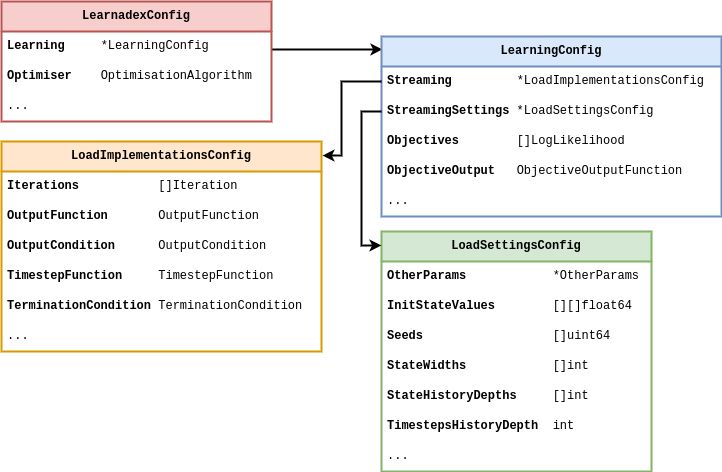
\includegraphics[width=7cm]{images/chapter-3-learnadex-data-types.drawio.png}
\caption{The learning config data type.}
\label{fig:learnadex-data-types-design}
\end{figure}

On the learning side; in order to define a specific objective for each data iterator to compute while the data streams through it, we have abstracted a `log-likelihood' type. Each data iterator is defined as a standard stochadex iteration, hence it can stream data into the learning algorithm from any user-defined source --- e.g., from a file on disk, from a local database instance or maybe via a network socket. In Fig.~\ref{fig:learnadex-data-iterator} below, we provide a schematic of the method calls of (and within) each data iterator.

\textcolor{red}{\begin{itemize}
\item{refactor the code and integrate the reweighting algorithm with Libtorch models for the conditional probabilities --- describe how this is supported}
\item{describe the method calls diagram in more detail --- in particular, point out how it can replace the \texttt{Iteration.Iterate} method which is called when the \texttt{StateIterator} is asked for another iteration from the \texttt{PartitionCoordinator} of the stochadex}
\item{then talk about the optimiser! starting with non-gradient-based: the two packages that are supported out of the box are gonum and eaopt (still need to do gago --- see here: github.com/maxhalford/eaopt) }
\item{also need to then support gradient-based algorithms (like vanilla SGD) by implementing Eq.~(\ref{eq:log-likelihood-reweighting-grad}) for the current basic implementations in the learnadex --- shouldn't be too difficult!}
\item{then talk about the output - talk about the possibilities for output and what the default setting to json logs is for}
\item{could also be written to, e.g., a locally-hosted database server and the best-suited would be a NoSQL document database, e.g., MongoDB~\cite{mongodb}, but building something bespoke and simpler is more aligned with the use-case here and with the principles of this book}
\item{describe the need for log exploration and visualisation and then introduce logsplorer - a REST API for querying the json logs (with basic filtering and selection capabilities but could be extended to more advanced options) and optionally also launches a visualisation React app written in Typescript}
\item{note how this could be scaled to cloud services easily and remotely queried through the logsplorer API and visualised} 
\end{itemize}}

\begin{figure}[h]
\centering
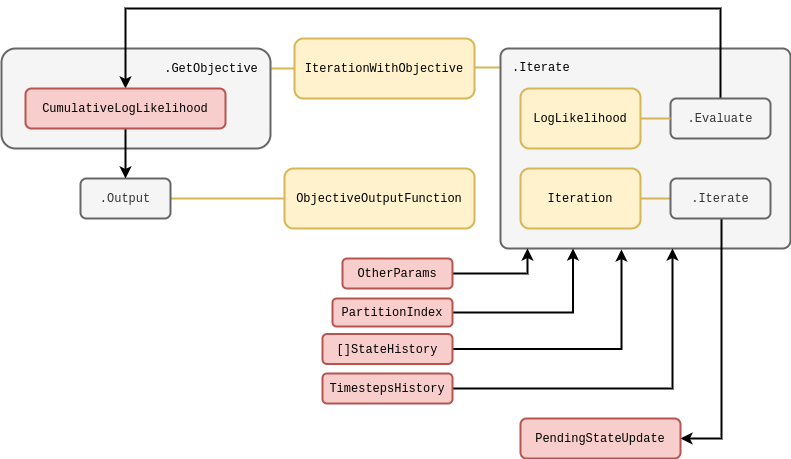
\includegraphics[width=14cm]{images/chapter-3-learnadex-data-iterator.drawio.png}
\caption{A schematic of an iteration with an objective function evaluation.}
\label{fig:learnadex-data-iterator}
\end{figure}

As with the software we wrote for the stochadex, the learnadex main binary executable leverages templating to enable full configurability of all the implementations and settings of Fig.~\ref{fig:learnadex-data-types-design} through passing configs at runtime. Users can alternatively use the learnadex as a library for import, if they desire more control over the code execution. 

\begin{figure}[h]
\centering
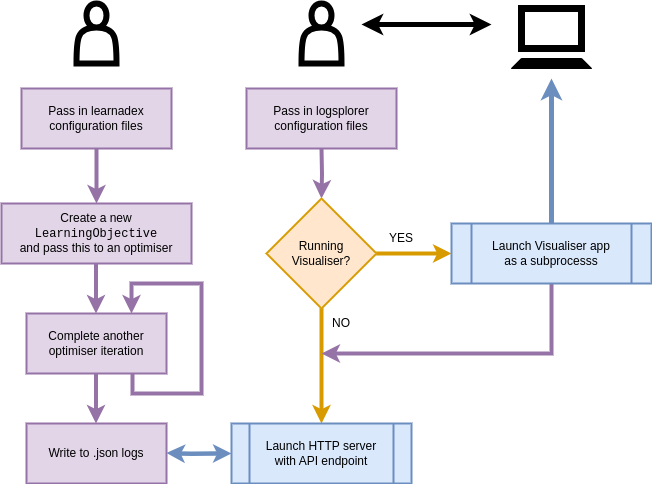
\includegraphics[width=13cm]{images/chapter-3-learnadex-main.drawio.png}
\caption{A diagram of the main learnadex and logsplorer executables.}
\label{fig:learnadex-main}
\end{figure}

\textcolor{red}{Take a step back at this point and consider all the use-cases for the learnadex:
\begin{itemize}
\item{Core functionality is to enable iterative updates to the $P_{\sf t}(X,z)$ distribution at every timestep. There must also be flexibility in how this distribution can represented, i.e., either:
\begin{itemize}
\item{a set of Monte Carlo samples, or}
\item{a set of distribution parameters}
\end{itemize}
}
\item{For Monte Carlo samples, we must also keep the flexibility to use either a BSL or ABC-style data-to-sim comparison in order to facilitate the update}
\item{For distribution parameters, the update can be custom-built by the user with online likelihood-based inference/Bayes estimator methods}
\item{Separate thread context runs of online learning methods using an update method, e.g.,}
\begin{itemize}
\item{Gradient-free batch optimisation with any chosen learning algorithm}
\item{Gradient-based parameter updates}
\item{Arbitrary parameter updates from a different method}
\end{itemize}
\end{itemize}}
    






\chapter{\sffamily Optimising interactions with any system}

{\bfseries\sffamily Concept.} To design and build software which enables the optimisation of automated control objectives over stochastic phenomena of any kind. The theory in this chapter will overlap significantly with that of Reinforcement Learning (RL), however, in contrast to more standard RL approaches, we shall be relying on all of the work from previous parts of this book to help agents characterise, measure and learn from their environment. The software which implements our generalised control optimisation algorithm will be implemented as an extension to the learnadex. For the mathematically-inclined, this chapter will cover how we formalise model-based automated control optimisation within the frameworks that we have already introduced in this book. For the programmers, the public Git repository for the code described in this chapter can be found here: \href{https://github.com/worldsoop/worldsoop}{https://github.com/worldsoop/worldsoop}.

\section{\sffamily Formalising general interactions}

Let's start by considering how we might adapt the mathematical formalism we have been using so far to be able to take actions which can manipulate the state at each timestep. Using the mathematical notation that we inherited from the stochadex, we may extend the formula for updating the state history matrix $X_{0:{\sf t}}\rightarrow X_{0:{\sf t}+1}$ to include a new layer of possible interactions which is facilitated by a new vector-valued `take action' function $G_{{\sf t}}$. In doing so we shall be defining the domain of an acting entity in the stochastic process environment --- which we shall hereafter refer to as simply the `agent'.

During a timestep over which actions are performed by the agent, the stochadex state update formula can be extended to include interactions by composition with the original state update function like so
%%
\begin{align}
X_{{\sf t}+1}^i &= G^i_{{\sf t}+1}[F_{{\sf t}+1}(X_{0:{\sf t}}, z, {\sf t}), A_{{\sf t}+1}] = {\cal F}^i_{{\sf t}+1}(X_{0:{\sf t}}, z, A_{{\sf t}+1}, {\sf t}) \label{eq:generalised-state-actions} \,,
\end{align}
%%
where we have also introduced the concept of the `actions' performed $A_{{\sf t}+1}$ on the system; some vector of parameters which define what actions are taken at timestep ${\sf t}+1$. The code for the new iteration formula would look something like Fig.~\ref{fig:iterations-with-actions}.

\begin{figure}[h]
\centering
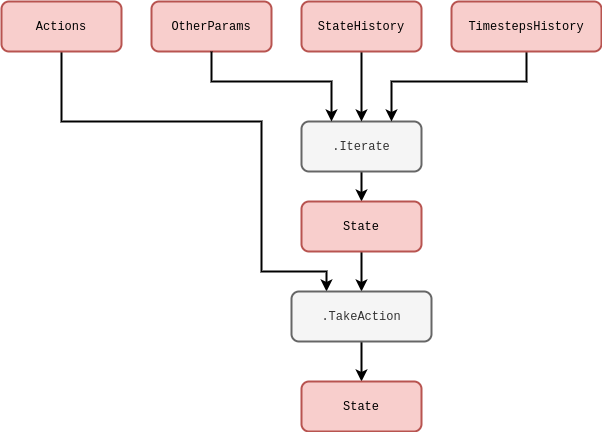
\includegraphics[width=11cm]{images/chapter-5-iterations-with-actions.drawio.png}
\caption{Code schematic of Eq.~(\ref{eq:generalised-state-actions}).}
\label{fig:iterations-with-actions}
\end{figure}

So far, Eq.~(\ref{eq:generalised-state-actions}) on its own will allow the agent to take actions that are scheduled up front through some fixed process or perhaps through user interaction via a game interface. So what's next? In order to start creating algorithms which will act on the system state for us, we need to develop a formalism which `closes the loop' by feeding information back from the stochastic process to the agent's decision-making algorithm.

If we use $A_{0:{\sf t}+1}$ a referring to the matrix of historically-taken actions which up to time ${\sf t}+1$, we can build up a more generalised, non-Markovian picture of automated interactions with the system which matches the notation we are already using for $X_{0:{\sf t}+1}$. Let us now define a Non-Markovian Decision Process (NMDP) as a probabilistic model which draws an actions matrix $A_{0:{\sf t}+1}=A$ from a `policy' distribution $\Pi_{({\sf t}+1){\sf t}}(A\vert X,\theta)$ given $X_{0:{\sf t}}=X$ and a new vector of parameters which fully specify the automated interations. Using the probabilistic notation from the previous part of the book, the joint probability that $X_{0:{\sf t}+1}=X$ and $A_{0:{\sf t}+1}=A$ at time ${\sf t}+1$ is
%%
\begin{align}
P_{{\sf t}+1}(X,A\vert z, \theta ) &= P_{{\sf t}}(X'\vert z,\theta ) \, \Pi_{({\sf t}+1){\sf t}}(A\vert X',\theta)P_{({\sf t}+1){\sf t}}(x\vert X',z,A) \label{eq:joint-prob-x-and-a} \,,
\end{align}
%%
where we recall that $P_{({\sf t}+1){\sf t}}(x\vert X',z,A)$ is the conditional probability of $X_{{\sf t}+1}=x$ given $X_{0:{\sf t}}=
X'$ and $z$ that we have encountered before, but it now requires $A_{0:{\sf t}+1}=A$ as another given input. We have illustrated Eq.~(\ref{eq:generalised-state-actions}) and how it relates to the policy distribution of Eq.~(\ref{eq:joint-prob-x-and-a}) with a new graph representation in Fig.~\ref{fig:fundamental-loop-with-actions}.

\begin{figure}[h]
\centering
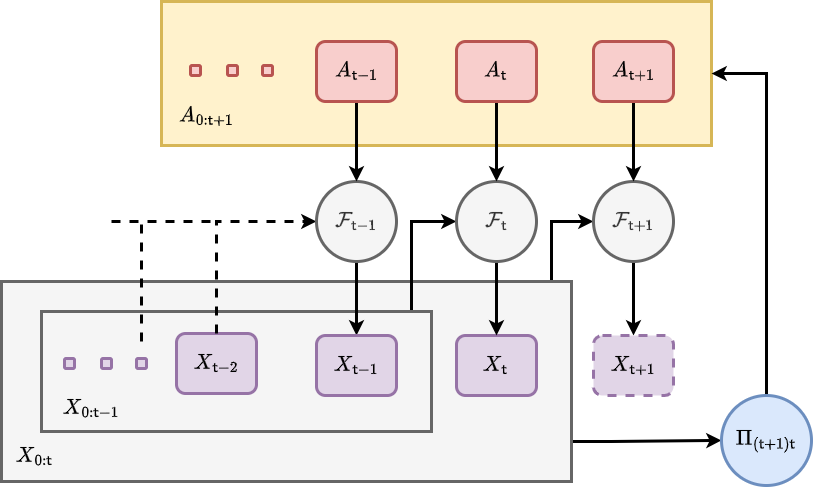
\includegraphics[width=11cm]{images/chapter-5-fundamental-loop-with-actions.drawio.png}
\caption{Graph representation of Eq.~(\ref{eq:generalised-state-actions}) with the policy distribution of Eq.~(\ref{eq:joint-prob-x-and-a}).}
\label{fig:fundamental-loop-with-actions}
\end{figure}

For additional clarity, let's take a moment to think about what $\Pi_{({\sf t}+1){\sf t}}(A\vert X,\theta)$ represents and how generally descriptive it can be. If an agent is acting under and entirely deterministic policy, then the policy distribution may be simplified to a direct function mapping which is parameterised by $\theta$. At the other extreme, the distribution may also describe a fully stochastic policy where actions are drawn randomly in time. If we combine this consideration of noise with the observation that policies described by a distribution $\Pi_{({\sf t}+1){\sf t}}(A\vert X,\theta)$ permit a memory of past actions and states, it's easy to see that this structure can be used in a wide variety of different use cases.

By marginalising over Eq.~(\ref{eq:joint-prob-x-and-a}) we find an updated probabilistic iteration formula for the stochastic process state which now takes the influence of agent actions into account
%%
\begin{align}
P_{{\sf t}+1}(X\vert z,\theta ) &= \int_{\Xi_{{\sf t}+1}}{\rm d}A \, P_{{\sf t}}(X'\vert z,\theta ) \, \Pi_{({\sf t}+1){\sf t}}(A\vert X',\theta)P_{({\sf t}+1){\sf t}}(x\vert X',z,A)  \,.
\end{align}
%%
This relationship will be very useful in the last part of this book when we begin to look at optimising control algorithms.

What are the main categories of action which are possible in the rows of $A$? Since the NMDP described by $\Pi_{({\sf t}+1){\sf t}}(A\vert X',\theta)$ is just another form of stochastic process, the main categories of action will fall into the same as those we covered in defining the stochadex formalism. The first, and perhaps most obvious, category would probably where the actions are defined in a continuous space and are continuously applied on every timestep. Some examples of these `continuously-acting' decision processes include controlling the temperature of chemical reactions~\cite{beeler2023chemgymrl} (such as those in a brewery), spacecraft control~\cite{tipaldi2022reinforcement} and guidance systems,  as well as the driving of autonomous vehicles~\cite{kiran2021deep}. Within a kind of subset of the continuously-acting category; we can also find the event-based acting decision processes (where actions are not necessarily taken every timestep), e.g. controlling traffic through signal timings~\cite{garg2018deep}, managing disease spread through treatment intervals~\cite{ohi2020exploring} and automated trading on stock markets~\cite{meng2019reinforcement}.

Many of the examples we have given above have continuous action spaces, but we might also consider classes of decision processes where actions are defined discretely. Examples of these include the famous multi-armed bandit problem~\cite{gittins2011multi} (like choosing between website layouts for E-commerce~\cite{liu2021map}), managing a sports team through player substitutions, sensor measurement scheduling~\cite{leong2020deep} and the sequential design prioritisation of large-scale scientific experiments~\cite{blau2022optimizing}.

\section{\sffamily States, actions and attributing rewards}

In the previous parts of this book we laid out the concept for a generalised framework to simulate and learn stochastic phenomena continually as data is received. Given that we have also introduced a framework for the automated control of these phenomena, we have all the ingredients we need to create optimal decision-making algorithms. The key question to answer then, is: \emph{optimal with respect to what objective?}

The objective of an automated control algorithm could take many forms depending on the specific context. Since there is no loss in generality in doing so, it seems natural to follow the naming convention used by Markov Decision Processes (MDP)~\cite{bertsekas2011dynamic,sutton2018reinforcement} by referring to the objective outcome of an action at a particular point in time as having a `reward' value $r$. Since the relationship between reward, actions and states may be stochastic, it makes sense to relate the reward outcome $r$ given a state history $X$ and action history $A$ at timestep ${\sf t}+1$ through the probability distribution $P_{{\sf t}+1}(r\vert X,A)$. Hence, generally, this reward signal is non-Markovian --- as is the case in many real-world problems~\cite{gaon2020reinforcement}. 

We can use the reward probability distribution to derive a joint distribution over both state history $X'$ and reward $r$ at timestep ${\sf t}+1$ like so
%%
\begin{align}
P_{({\sf t}+1){\sf t}}(r,x'\vert X, z,\theta) &= P_{{\sf t}+1}(r\vert X',A)\Pi_{({\sf t}+1){\sf t}}(A\vert X,\theta)P_{({\sf t}+1){\sf t}}(x'\vert X,z,A) \label{eq:joint-x-and-r}\,.
\end{align}
%%
In this expression, let's recall that we are using the policy distribution $\Pi_{({\sf t}+1){\sf t}}(A\vert X,\theta)$ for agent interactions and the fundamental state update conditional probability for the underlying stochastic process $P_{({\sf t}+1){\sf t}}(x'\vert X,z,A)$.

Note that in most use cases, the state of real-world phenomena cannot be measured perfectly. So to enable any agent trained on simulated phenomena to potentially act in the real world, we will need to include a measurement process as part of the information retrieval step. This is the part where we can leverage our work in a previous chapter which develops an online learning system for stochastic process models. But we're jumping ahead with this thinking and will return to this point later on.

Using Eq.~(\ref{eq:joint-x-and-r}), we can now define a `state value function' $V_{{\sf t}}$ at timestep ${\sf t}$ which is the expected $\gamma$-discounted future reward given the current state history $X$ and the other parameters like this\footnote{The discount factor in continuous time could also be explicitly dependent on the stepsize such that we would replace the discount factor in Eq.~(\ref{eq:state-value-discounted-return}) with
$$
\gamma^{{\sf t}'-{\sf t}} \longrightarrow \frac{1}{\gamma [\delta t({\sf t}+1)]}\prod_{{\sf t}''={\sf t}}^{{\sf t}'} \gamma [\delta t({\sf t}''+1)] \,.
$$}
%%
\begin{align}
V_{{\sf t}}(X,z,\theta) &= {\rm E}_{{\sf t}}({\sf Discounted \,Return}\vert X, z, \theta ) \nonumber \\
&= \sum_{{\sf t}'={\sf t}}^{\infty} \int_{\omega_{{\sf t}'+1}}{\rm d}^nx'\int_{\rho_{{\sf t}'+1}} {\rm d}r \,r\, \gamma^{{\sf t}'-{\sf t}}\prod_{{\sf t}''={\sf t}}^{{\sf t}'}P_{({\sf t}''+1){\sf t}''}(r,x'\vert X, z,\theta) \label{eq:state-value-discounted-return}\,,
\end{align}
%%
where $0 < \gamma < 1$. The idea behind this discount factor $\gamma$ is to decrease the contribution of rewards to the optimisation objective (often called the `expected discounted return' in RL) more and more as the prediction increases into the future. Note also that the state value function is inherently recursively defined, such that
%%
\begin{align}
V_{{\sf t}}(X,z,\theta) &= \int_{\omega_{{\sf t}+1}}{\rm d}^nx\int_{\rho_{{\sf t}+1}} {\rm d}r \, P_{({\sf t}+1){\sf t}}(r,x'\vert X, z,\theta)\bigg\{ r+\gamma V_{{\sf t}+1}(X',z,\theta)\bigg\} \,,
\end{align}
%%
and the optimal $\theta$ can hence be derived from
%%
\begin{align}
\theta^*_{{\sf t}}(X,z) &= \underset{\theta}{{\rm argmax}} \big[ V_{{\sf t}}(X,z,\theta)\big] \,.
\end{align}
%%
By deriving the optimal policy in terms of the parameters $\theta^*_{{\sf t}}(X,z)$, the optimal state value function and policy distribution can therefore be derived from
%%
\begin{align}
V^*_{{\sf t}}(X,z) &= V_{{\sf t}}[X,z,\theta^*_{{\sf t}}(X,z)] \\
\Pi^*_{({\sf t}+1){\sf t}}(A\vert X,z) &= \Pi_{({\sf t}+1){\sf t}}[A\vert X,\theta^*_{{\sf t}}(X,z)] \,.
\end{align}
%%

Note that the type of decision process optimisation which we have introduced above differs from standard RL methodology. In the more conventional `model-free' RL approaches, the state-action value function 
%%
\begin{align}
Q_{{\sf t}}(X,A,z)={\rm E}_{{\sf t}}({\sf Discounted \,Return}\vert X,A,z) \,,
\end{align}
%%
would be used to evaluate the optimal policy instead of the state value function $V_{{\sf t}}(X,z,\theta )$ that we are using above. We are able to use the latter here because the simulation model gives us explicit knowledge of the $P_{({\sf t}+1){\sf t}}(x'\vert X,z,A)$ distribution which is utilised by Eq.~(\ref{eq:joint-x-and-r}). When this model is not known, the state-action value function $Q_{{\sf t}}(X,A,z)$ must be learned explicitly through sample estimation from the measured state and experienced outcomes of actions taken by the agent.

When an agent takes an action to measure the state of the system (or when it is given measurements without needing to take action) there will typically be some uncertainty in how the history of measured real-world data $Y$ maps to the latent states of the system $X$ and its parameters $z$ at time ${\sf t}+1$. It is natural, then, to represent this uncertainty with a posterior probability distribution ${\cal P}_{{\sf t}+1}(X,z\vert Y)$ as we did in the previous chapters of this book.

\section{\sffamily Algorithm designs}

\textcolor{red}{
Follow-up this bit with the model-based approach that we're going to take in this book.
\begin{itemize}
\item{Introduce broad concept of dynamic programming --- partitioning a optimal global control into smaller optimal control segments/iterations.}
\item{Talk about the utility of the model-based online learning approach in the case of partially observed systems~\cite{aastrom1965optimal}.}
\item{Look into the overlaps with this approach and Thompson sampling for exploration --- discuss here.}
\item{Looking at a stochastic policy iteration algorithm here combined with Monte Carlo rollouts.}
\item{The value learning can be facilitated in software using a predictive model which is able to roll forecast rewards forward in time in a Monte Carlo fashion up to a window from a certain point given an input prior distribution of policies.}
\item{This input prior distribution of policies can itself be optimised by maximising expected discounted utility in a Bayesian design framework. Draw parallels.}
\end{itemize}
}

\section{\sffamily Software design}

\begin{figure}[h]
\centering
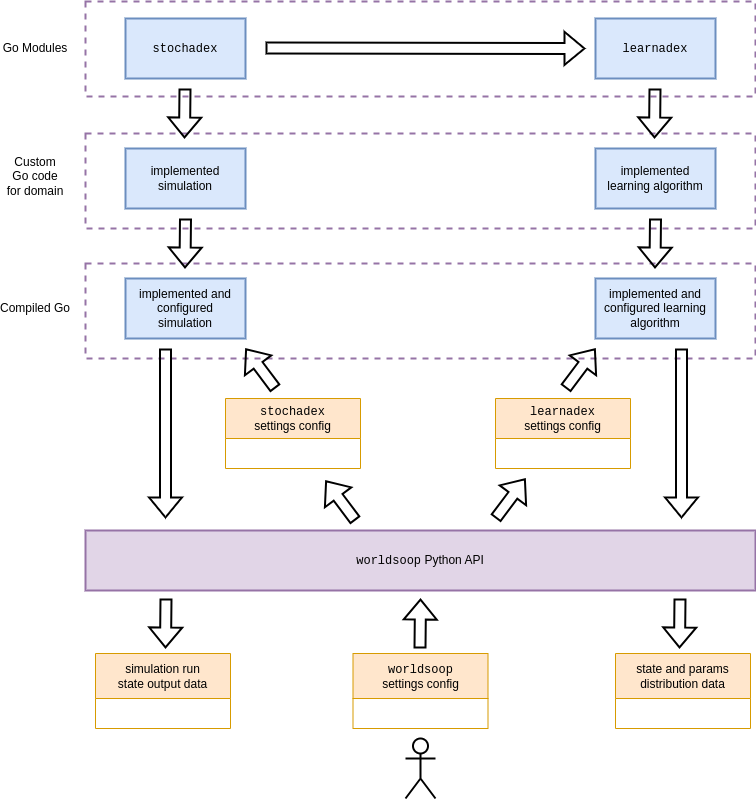
\includegraphics[width=11cm]{images/chapter-5-high-level-dependencies.drawio.png}
\caption{Diagram illustrating the high-level layer inter-dependencies of the Python API.}
\label{fig:high-level-api-dependencies}
\end{figure}

\part*{{\sffamily Part 2}}

\chapter{\sffamily Controlling parasitic infections}

{\bfseries\sffamily Concept.} The idea here is to limit the spread of some abstract spatial parasitic infections through the correct time-dependent resource allocation.

\section{\sffamily Adapting the probabilistic formalism}

Let's by returning to the probabilistic formalism that we introduced earlier and noting that the covariance matrix estimate with elements $C^{ij}_{{\sf t}+1}(z)$ represents a matrix that could get very large, depending on the problem. For example; if we encoded the state of a 2-dimensional spatial field of values into the elements $X^i_{\sf t}$, the number of elements in the covariance matrix $C^{ij}_{{\sf t}+1}(z)$ would scale as $4N^2$ --- where $N$ here is the number of spatial points we wanted to encode. 

One solution to this scaling problem is to exploit the fact that, in many spatial processes, the proximity of points can strongly determine how correlated they are. Hence, for pairwise distances further than some threshold, the covariance matrix elements should tend towards 0. If we were to place points along the diagonal of $C^{ij}_{{\sf t}+1}(z)$ in order of how close they are to each other, this threshold would then be represented as a \emph{banded matrix}. We have illustrated such a matrix in Fig.~\ref{fig:banded-matrix} in which the `bandwidth' is defined as the number of diagonals one needs to traverse from the main diagonal before encountering a diagonal of 0s.

\begin{figure}[h]
\centering
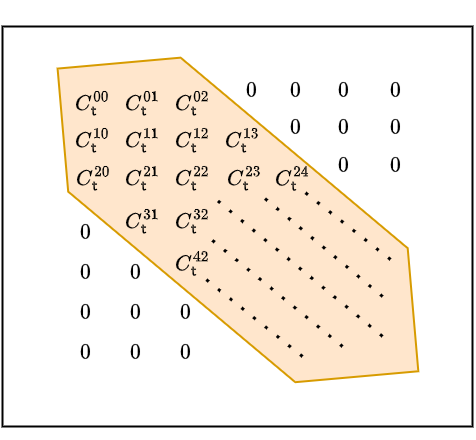
\includegraphics[width=9cm]{images/chapter-6-banded-matrix.drawio.png}
\caption{An illustration of a banded covariance matrix with a bandwidth of 2.}
\label{fig:banded-matrix}
\end{figure}

\textcolor{red}{
\begin{itemize}
\item{Full sim: fully individual-based spatial stochastic model}
\item{Inference model: spatial mean field inference features using the probabilistic reweighting + exponentially-weighted nonlinear features}
\item{Also use the likelihood-free inference model}
\end{itemize}
}

\textcolor{red}{
\begin{itemize}
\item{At some point it might be sensible to move into the Fourier domain here --- at least for derivations and calculations. Probably more intuitive for the reader to keep it mostly in real space though if possible.} 
\item{The extra detail that's also needed here is to consider how we encode a 2-dimensional spatial process into our state vector, and how the elements of the resulting state vector might be correlated to one another depending on their spatial proximity. If we start with a Markovian Gaussian random field, we can derive the Mat\'{e}rn kernel over these spatial coordinates in order to correlate the state vectors in such a way.} 
\item{Also look into the Radial Basis Function (RBF) and higher-order derived kernels based on DALI expansion~\cite{sellentin2014breaking} in order to try and capture non-Gaussianity.}
\item{Spatial malaria models here:~\cite{smith2008towards,djordjevic2022stochastic}}
\item{Spatial helminth-like infections too would be a good template...}
\end{itemize}
}


\chapter{\sffamily Algo-trading on financial markets}

{\bfseries\sffamily Concept.} The idea here is to use the Q-Hawkes processes and the Bouchaud work to come up with some interesting simulations of financial markets. 

\section{\sffamily Introducing Q-Hawkes processes}



\chapter{\sffamily Sustainable angling for fish}

{\bfseries\sffamily Concept.} The idea here is 

\section{\sffamily A large-scale Lotka-Volterra model}

Inspired by the empirical dynamical modeling approach to sockeye salmon in Ref.~\cite{ye2015equation}, but also desiring a generative model which has some link to the classic causal models promoted by mathematical ecology; the goal here is to create and calibrate a stochastic model which predicts the fish counts, weights, lengths and ages for each species in each area based on the past system states. To do this, we will combine some well-known models from mathematical ecology with supervised learning.

The one-step master equation for the proposed stochastic simulation is given implictly by

\begin{align}
\frac{{\rm d}}{{\rm d} t} P(\dots, n_{i}, \dots, t) &= \sum_{\forall i}{\cal T}^{+}_{i}(\dots, n_i-1, \dots, {\sf f}, t)P(\dots, n_{i}-1, \dots, t) \\
&+ \sum_{\forall i}{\cal T}^{-}_{i}(\dots, n_i+1, \dots, {\sf f}, t)P(\dots, n_{i}+1, \dots, t) \\
&- \sum_{\forall i}\bigg[ {\cal T}^{+}_{i}(\dots, n_i, \dots, {\sf f}, t) + {\cal T}^{-}_{i}(\dots, n_i, \dots, {\sf f}, t) \bigg] P(\dots, n_{i}, \dots,t) \,,
\end{align}

where the time $t$ is defined in units of years and ${\cal T}^{+}_{i}$ and ${\cal T}^{-}_{i}$ are the transition coefficients for the $i$-th species, which depend not only on the counts for all species $n_1, n_2, \dots$, but also (in principle) on a larger feature space ${\sf f}$ generated by the available data up to time $t$.

The famous Lotka-Volterra system, with some modficiations for fishing and a larger set of species, would suggest transition coefficients of the form


\begin{align}
{\cal T}^{+}_{i}(\dots, n_i, \dots, {\sf f}, t) = {\cal T}^{+}_{i}(\dots, n_i, \dots) &= \Lambda_{i}(n_{i}) + n_{i}\alpha_{i}\sum_{\forall i' \, {\sf prey}}n_{i'}\\
{\cal T}^{-}_{i}(\dots, n_i, \dots, {\sf f}, t) = {\cal T}^{-}_{i}(\dots, n_i, \dots) &= n_{i}\mu_{i} +  n_{i}\gamma_{i} + n_{i}\beta_{i} \sum_{\forall i' \, {\sf pred}} n_{i'} \,,
\end{align}


where: $\Lambda_{i}(n_{i}) = \tilde{\Lambda_{i}}n_{i}e^{-\lambda_i(n_{i}-1)}$ is the density-dependent birth rate; $\mu_{i}$ is the species death rate; $\alpha_{i}$ is the increase in the baseline birth rate per fish caused by the increase in prey population; $\beta_{i}$ is the rate per fish of predation of the species; and $\gamma_{i}$ accounts for the rate of recreational fishing per fish of the species. To approach the present data-driven simulation problem, we're going to generalise this model by training ${\cal T}^{+}_{i}(\dots, n_i, \dots, {\sf f}, t)$ and ${\cal T}^{-}_{i}(\dots, n_i, \dots, {\sf f}, t)$ directly from the data and generated features.

Look into the likelihood from, e.g., an electrofishing survey such as in Ref.~\cite{envagency2015}...

\begin{align}
{\sf Likelihood} &= \sum_{{\sf data}}{\rm NB}\big[{\sf data};w_{i,{\sf survey}}\langle n_i(t_{{\sf data}})\rangle,k_{i,{\sf survey}}\big] \,,
\end{align}

\chapter{\sffamily Managing a rugby match}

{\bfseries\sffamily Concept.} Building a toy model simulation of a rugby match whose outcome can be manipulated through correctly-timed player substitutions and game management decisions. The dexetera state manipulation framework we have built around the stochadex can meet these requirements, and a dashboard can be created for user interaction. All this combines together to make a simple dashboard game, which we call: `trywizard'. For the mathematically-inclined, this chapter will motivate the construction of a specific modelling framework for rugby match simulation. For the programmers, the public Git repository for the code described in this chapter can be found here: \href{https://github.com/umbralcalc/trywizard}{https://github.com/umbralcalc/trywizard}.

\section{\sffamily Designing the event simulation engine}

Since the basic state manipulation framework and simulation engine will run using \href{https://github.com/umbralcalc/dexetera}{dexetera}, the mathematical novelties in this project are all in the design of the rugby match model itself. And, as ever, we're not especially keen on spending a lot of time doing detailed data analysis to come up with the most realistic values for the parameters that are dreamed up here. Even though this would also be interesting.\footnote{One could do this data analysis, for instance, by scraping player-level performance data from one of the excellent websites that collect live commentary data such as \href{https://www.rugbypass.com/}{rugbypass.com} or \href{https://www.espn.co.uk/rugby/}{espn.co.uk/rugby}.}

Let's begin by specifying an appropriate state space to live in when simulating a rugby match. It is important at this level that events are defined in quite broadly applicable terms, as it will define the state space available to our stochastic sampler and hence the simulated game will never be allowed to exist outside of it. It seems reasonable to characterise a rugby union match by the following set of states: {\sf Penalty}, {\sf Free Kick} (the punitive states); {\sf Penalty Goal}, {\sf Drop Goal}, {\sf Try} (the scoring states); {\sf Kick Phase}, {\sf Run Phase}, {\sf Knock-on}, {\sf Scrum}, {\sf Lineout}, {\sf Maul} and {\sf Ruck} (the general play states). Using this set of states, in Fig.~\ref{fig:event-graph} we have summarised our approach to match state transitions into a single event graph. In order to capture the fully detailed range of events that are possible in a real-world match, we've needed to be a little imaginative in how we define the kinds of state transitions which occur. In other words; it's fair to say that our simplified model here represents just a subset of states that a real rugby match could exist in.

\begin{figure}[h]
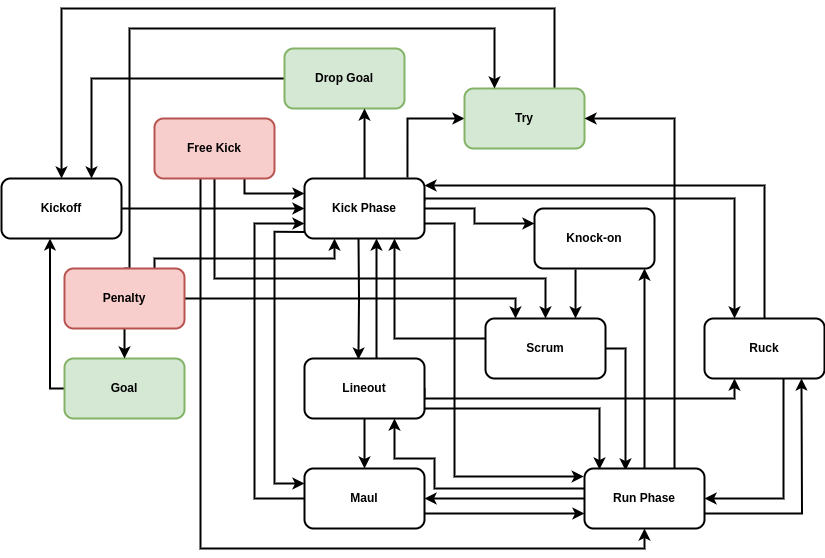
\includegraphics[width=14cm]{images/trywizard-event-graph.drawio.png}
\caption{Simplified event graph of a rugby union match.}
\label{fig:event-graph}
\end{figure}

In addition to occupying some state in the event graph, the state of a rugby match must also include a binary `possession' element which encodes which team has the ball at any moment. We should also include the 2-dimensional pitch location of the ball as an element of the match state in order to get a better sense of how likely some state transitions are, e.g., when playing on the edge of the pitch near the touchline it's clearly more likely that a {\sf Run Phase} is going to result in a {\sf Lineout} than if the state is currently in the centre of the pitch. To add even more detail; in the next section we will introduce states for each player.

Since a rugby match exists in continuous time, it is natural to choose a continuous-time event-based simulation model for our game engine. As we have discussed in previous chapters already, this means we will be characterising transition probabilities of the event graph in Fig.~\ref{fig:event-graph} by ratios of event rates in time. Recalling our notation in previous chapters, if we consider the current state vector of the match $X_{\sf t}$, we can start by assigning each transition ${\sf a}\rightarrow {\sf b}$ on the event graph an associated expected rate of occurance $\lambda_{{\sf a}\rightarrow {\sf b}}$ which is defined in units of continuous time, e.g., seconds. In addition to the transitions displayed on the graph, we can add a `possession change transition'; where the possession of the ball in play moves to the opposing team. This transition may occur while the match is also in any of the white-coloured states on the graph (apart from {\sf Knock-on} which determines a possession change immediately through a {\sf Scrum}) and let's assign this a state, parameter and timestep-dependent expected rate of occurance $\lambda_{\rm pos}(X_{\sf t}, z, {\sf t})$.

Based on our dicussion above, an appropriate encoding for the overall game state at timestep index ${\sf t}$ could be a state vector $X_{{\sf t}}$ whose elements are
%%
\begin{align}
X^0_{{\sf t}}&=\begin{cases} 0 & \text{Match State} = \text{{\sf Penalty}}\\ 1 & \text{Match State} = \text{{\sf Free Kick}} \\ \dots & \end{cases} \\
X^1_{{\sf t}}&=\begin{cases} 0 & \text{Possession} = \text{{\sf Home Team}}\\ 1 & \text{Possession} = \text{{\sf Away Team}} \end{cases} \,.
\end{align}
%%
But how does this overall game state connect to the event rates? The probabilistic answer is quite straightforward. If the probability of the match state being $X^0_{{\sf t}}={\sf a}$ at timestep ${\sf t}$ is written as $P^0_{{\sf t}}({\sf a})$, then the probability of $X^0_{{\sf t}+1}={\sf b}$ in the following timestep is
%%
\begin{align}
P^0_{{\sf t}+1}({\sf b}) = \frac{\frac{1}{\tau}P^0_{{\sf t}}({\sf b})+\sum_{\forall {\sf a}\neq {\sf b}}\lambda_{{\sf a}\rightarrow {\sf b}}{\cal T}_{{\sf a}\rightarrow {\sf b}}(X_{\sf t}, z, {\sf t})P^0_{{\sf t}}({\sf a})}{\big[ \frac{1}{\tau} + \sum_{\forall {\sf a}\neq {\sf b}}\lambda_{{\sf a}\rightarrow {\sf b}} {\cal T}_{{\sf a}\rightarrow {\sf b}}(X_{\sf t}, z, {\sf t})\big]} \label{eq:match-state-transition-probs}\,,
\end{align}
%%
where $\forall {\sf a} \neq {\sf b}$ in the summation indicates that all the available transitions from ${\sf a}$ to ${\sf b}$, where ${\sf a}\neq {\sf b}$, should be summed over and ${\cal T}_{{\sf a}\rightarrow {\sf b}}(X_{\sf t}, z, {\sf t})$ is a time, parameter and state-dependent transition probability that is determined by the playing tactics of each team as well as the general likelihoods of gameplay which are expected from a real rugby match. Note that in the expression above, we have also defined $\tau$ as a timescale short enough such that no transition is likely to occur during that interval. An equivalent to Eq.~(\ref{eq:match-state-transition-probs}) should also apply to the possession change transition rate, i.e., the probability that the {\sf Home Team} has possession $P^1_{{\sf t}}$ at time ${\sf t}$ evolves according to
%%
\begin{align}
P^1_{{\sf t}+1} = \frac{ \frac{1}{\tau}P^1_{{\sf t}} + \lambda_{\rm pos}(X_{\sf t}, z, {\sf t}) (1-P^1_{{\sf t}})}{\big[ \frac{1}{\tau} + \lambda_{\rm pos}(X_{\sf t}, z, {\sf t})\big]} \label{eq:possession-change-probs}\,.
\end{align}
%%

Before we move on to other details, it's quite important to recognise that because our process is defined in continuous time, the possession change rate may well vary continuously (this will be especially true when we talk about, e.g., player fatigue). Hence, Eq.~(\ref{eq:match-state-transition-probs}) is only an \emph{approximation} of the true underlying dynamics that we are trying to simulate --- and this approximation will only be accurate if $\tau$ is small. The reader may recall that we discussed this same issue from the point of view of simulating time-inhomogeneous Poisson processes with the rejection method when we were building the stochadex in an earlier chapter. 

While these match state transitions and possession changes are taking place, we also need to come up with a model for how the ball location $L_{{\sf t}}$ changes during the course of a game, and as a function of the current game state. Note that, because the ball location is a part of the overall game state, it will be included as information contained within some elements of $X_{{\sf t}}$ as well. To make this explicit, we can simply set $X^2_{{\sf t}}=L^{\rm lon}_{{\sf t}}$ and $X^3_{{\sf t}}=L^{\rm lat}_{{\sf t}}$ --- where $L^{\rm lon}_{{\sf t}}$ denotes the longitudinal component (lengthwise along the pitch) and $L^{\rm lat}_{{\sf t}}$ denotes the lateral component (widthwise across the pitch). If we associate every state on the event graph with a single change in spatial location of the ball on the pitch, we then need to construct a process which makes `jumps' in 2-dimensional space each time a state transition occurs. To keep things simple and intuitive, we will say that movements of the ball are only allowed to occur during either a {\sf Run Phase} or a {\sf Kick Phase}. 

In the case of a {\sf Run Phase}, let's choose the longitudinal component of the ball location $L^{\rm lon}_{{\sf t}}$ to be updated by the difference between samples drawn from two exponential distributions (one associated to each team). Hence, the probability density $P_{{\sf t}}(\ell )$ of $L^{\rm lon}_{{\sf t}}=\ell$ at timestep ${\sf t}$ evolves according to
%%
\begin{align}
P_{{\sf t}+1}(\ell ) = \int^\infty_0 {\rm d}\ell'\, {\sf ExponentialPDF}(\ell + \ell'; a_{\rm run}){\sf ExponentialPDF}(\ell'; d_{\rm run}) \label{eq:longitudinal-motion-rugby} \,,
\end{align}
%%
where $a_{\rm run}$ and $d_{\rm run}$ are the exponential distribution scale parameters for an attacking and defending player, respectively, and we have chosen positive values of $\ell$ to be aligned with the forward direction for the attacking team. We shall elaborate on where $a_{\rm run}$ and $d_{\rm run}$ come from when we discuss associating events for player abilities in due course. If we now consider lateral component of the ball location $L^{\rm lat}_{{\sf t}}$ during a {\sf Run Phase}; it makes sense that this wouldn't be affected much by either team within the scope of detail in this first version of our model. Hence, the probability density $P_{{\sf t}}(w)$ of $L^{\rm lat}_{{\sf t}}=w$ at timestep ${\sf t}$ can just be updated like so
%%
\begin{align}
P_{{\sf t}+1}(w) = {\sf NormalPDF}(w; L^{\rm lat}_{{\sf t}}, \sigma_{\rm run}^2) \label{eq:lateral-motion-rugby} \,,
\end{align}
%%
where $\sigma_{\rm run}$ is the typical jump in lateral motion (the standard deviation parameter of the normal distribution).

Turning our attention to the {\sf Kick Phase}; the longitudinal component is only realistically controlled by the attacking team. There's also an angular component to this motion which is associated to the direction that the kicker is orientating their kick. Therefore, the probability density of $P_{{\sf t}}(\ell )$ with $L^{\rm lon}_{{\sf t}}=\ell \cos \theta$ and $L^{\rm lat}_{{\sf t}}=\ell \sin \theta$ at timestep ${\sf t}$ will evolve according to
%%
\begin{align}
P_{{\sf t}+1}(\ell ) = {\sf ExponentialPDF}(\ell; a_{\rm kick}) \label{eq:longitudinal-motion-rugby-kicking} \,,
\end{align}
%%
where $a_{\rm kick}$ this time is the exponential scale parameter for the attacking team player who is kicking and $\theta$ is the angle they have chosen to kick at (where straight ahead is defined as $\theta = 0$). Similarly, the lateral component for a {\sf Kick Phase} is only going to be controlled by the accuracy of the kicker with the angle and longitudinal distance already applied. Therefore, the corresponding update to the probability density $P_{{\sf t}}(w)$ where $L^{\rm lon}_{{\sf t}}=w \sin \theta$ and $L^{\rm lat}_{{\sf t}}=w \cos \theta$ at timestep ${\sf t}$ will look like
%%
\begin{align}
P_{{\sf t}+1}(w) = {\sf NormalPDF}(w; L^{\rm lat}_{{\sf t}} + \ell \sin \theta, \sigma_{\rm kick}^2) \label{eq:lateral-motion-rugby-kicking} \,,
\end{align}
%%
with a standard deviation $\sigma_{\rm kick}$, and its interpretation now being the accuracy of the kicker.

\section{\sffamily Associating events to player states and abilities}

In the last section we introduced a continuous-time event-based simulation model for a rugby union match. In this section we are going to add more detail into this model by inventing how to associate specific player states and abilities to the event rates of the simulation. Before continuing, we want to reiterate that this model is entirely made up and, while we hope it illustrates some interesting mathematical modelling ideas in the context of rugby, there's no particular reason why a statistical inference with a reliable dataset should prefer our model to others which may exist.

In Fig.~\ref{fig:player-abilities} we began by separating playing positions on the rugby field into their usual descriptions and then associating each player type with a short list of simplified attributes. Our model is then to associate a player with an `possession attacking' and `possession defending' ability which corresponds to each of their attributes. For example, a Front Row Forward will have 8 abilities associated to them: 2 for each of their {\sf Scrum}, {\sf Lineout}, {\sf Ruck} and {\sf Maul} attributes.

\begin{figure}[h]
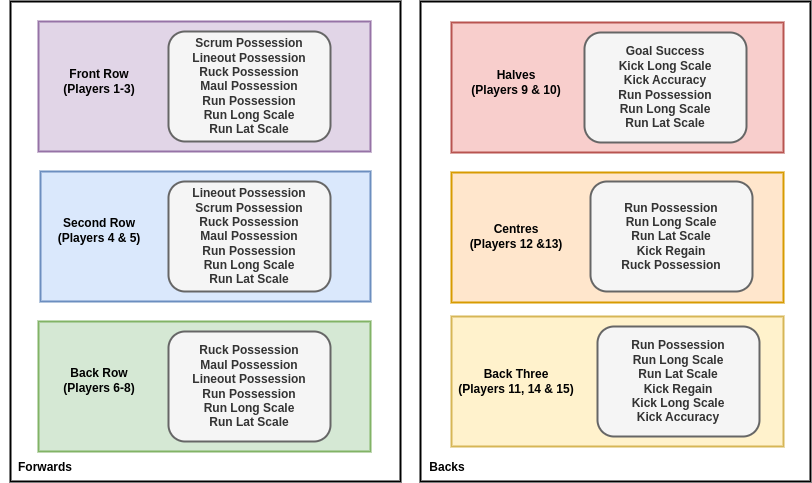
\includegraphics[width=15cm]{images/rugby-player-abilities.drawio.png}
\caption{Associated playing abilities for each position type.}
\label{fig:player-abilities}
\end{figure}

Let's now say that $z$ contains all of these parameters for all of the players on both sides, and also whether or not each player is actively playing or on the bench. With this information, and the knowledge of which team is in possession from $X^1_{\sf t}$, it should be simple to create a vector-valued function $a_{\rm pos}(X_{\sf t}, z)$ which returns all of the posession attacking attributes that are associated to match state $X^0_{\sf t}$ and an analogous one $d_{\rm pos}(X_{\sf t}, z)$ for the possession defending attributes. The dependencies of these functions on the ball possession state $X^1_{\sf t}$ comes from the fact that when, e.g., the {\sf Home Team} has possession of the ball it will be their possession attacking attributes that are returned by $a_{\rm pos}(X_{\sf t}, z)$ and the {\sf Away Team}'s possession defending attributes that are returned by $d_{\rm pos}(X_{\sf t}, z)$.

In order to model the effect of player fatigue over the course of a match, we can add some vectors of player fatigue values $f$ and times at which each player started playing $t_{\rm start}$ into the collection of parameters that are contained within $z$. These new parameters can then be used to define a formula for the decline of each attribute over the course of a match. Let's assign these declining values to be part of the overall match state like so
%%
\begin{align}
X^j_{\sf t} &= a^j_{\rm pos}(X_{\sf t}, z)e^{-f^j[t({\sf t})-t^j_{\rm start}]} \label{eq:att-player-fatigue} \\
X^k_{\sf t} &= d^k_{\rm pos}(X_{\sf t}, z)e^{-f^k[t({\sf t})-t^k_{\rm start}]} \label{eq:def-player-fatigue} \,,
\end{align}
%%
where the $j$ and $k$ each index the range of indices in the overall match state which correspond to the attacking and defending team player states, respectively.

So how does each player affect the events of a match? In our model, we would argue that players should be able to directly influence the possession change rate $\lambda_{\rm pos}(X_{\sf t}, z, {\sf t})$ through a balance of attacking and defensive attributes in the following relation
%%
\begin{align}
\lambda_{\rm pos}(X_{\sf t}, z, {\sf t}) &= \frac{\lambda^*_{\rm pos}\sum_{\forall j}X^j_{{\sf t}}}{\sum_{\forall j}X^j_{{\sf t}} + \sum_{\forall k}X^k_{{\sf t}}}\,,
\end{align}
%%
where $\lambda^*_{\rm pos}$ is the maximum rate that is physically possible and the $\forall j$ and $\forall k$ in the summations indicate summing over all attacking and defending player attributes, respectively. In addition to this possession change influence, players who have {\sf Run Phase} and {\sf Kick Phase} attributes may affect the gain in distance (and accuracy in the case of {\sf Kick Phase}) that each state translates to on the pitch. 

Let's first describe how we intend the {\sf Run Phase} to work. Every time the match state transitions into a {\sf Run Phase}, an individual player on the attacking side is chosen at random (uniformally across the team\footnote{This uniform sampling could be refined later to associate sampling probabilities with game state and player roles.}) to be the the nominal `attacker'. At the same time, an individual player on the defending side is chosen at random (again, uniformally across the team) to be the the nominal `defender'. Once these players have been chosen (and hence the $a_{\rm run}$ and $d_{\rm run}$ parameters have been determined), the longitudinal motion update we described in Eq.~(\ref{eq:longitudinal-motion-rugby}) can then be applied. Note that the $a_{\rm run}$ and $d_{\rm run}$ parameters should also receive a fatigue decrement depending on the time that each player has remained on the pitch, much like the exponential factors we applied in Eqs.~(\ref{eq:att-player-fatigue}) and~(\ref{eq:def-player-fatigue}).

Finally, we turn or attention to the mechanics of a {\sf Kick Phase}. For tactical kicking in the middle of play, this operates in a similar way as a {\sf Run Phase}; one of the players on the attacking side (the side in possession of the ball) is chosen at random (uniformally) and their $a_{\rm kick}$ and $\sigma_{\rm kick}$ attributes are used in Eqs.~(\ref{eq:longitudinal-motion-rugby-kicking}) and~(\ref{eq:lateral-motion-rugby-kicking}) to update the position of the ball. In the specific case of {\sf Goal} kicking from a {\sf Penalty}, the designated place kicker on each side also uses their same {\sf Kick Phase} attributes to determine the success/failure of the kick at the posts.

\section{\sffamily Deciding on managerial actions}

So how does managing a rugby match map to measured states and taking actions? To begin with, it makes sense to claim that the measurement of the total match state is perfect in this instance, and hence ${\cal S}_{{\sf t}}=X_{{\sf t}}$. We then have to figure out what sorts of managerial actions ${\cal A}_{{\sf t}}$ are parametric in nature (affecting $z$) and if any directly act on the state of the system itself (affecting $X_{\sf t}$). Let's jump straight to the answer to the second question --- we can't really think of any situation where the overall match state $X_{\sf t}$ itself is directly changed by a managerial action, so we will be using only parametric actions in this chapter.

Our model structure would suggest that the only way in which a manager can influence the state of a match is through modifying the parameters which are used by the $a_{\rm pos}(X_{\sf t},z)$, $d_{\rm pos}(X_{\sf t},z)$ or ${\cal T}_{{\sf a}\rightarrow {\sf b}}(X_{\sf t},z,{\sf t})$ functions. In the case of the possession attacking and defending attributes $a_{\rm pos}(X_{\sf t},z)$ and $d_{\rm pos}(X_{\sf t},z)$, a parametric action that the manager can perform would be to modify which players are actively playing through substitutions. To indicate that this underlying data may change, one can simply promote $z$ to its actionable, time-dependent counterpart $Z_{{\sf t}}$.

In addition to the changes that we have discussed above, we would argue that the parameters $a_{\sf run}$, $d_{\sf run}$, $a_{\rm kick}$ and $\sigma_{\rm kick}$ in Eqs.~(\ref{eq:longitudinal-motion-rugby}), (\ref{eq:longitudinal-motion-rugby-kicking}) and (\ref{eq:lateral-motion-rugby-kicking}) can also be determined by the manager to some extent through player selection/substitutions. 

\section{\sffamily Writing the game itself}

\begin{itemize}
\item{Show which stochadex/dexetera methods were called and how they were used to simulate the game.}
\item{Give a summary of how the dashboard backend works (diagram would help) and how this connects up to the streamlit frontend via protobuf messages.}
\end{itemize}

\chapter{\sffamily Optimising relief chain logistics}

{\bfseries\sffamily Concept.} The idea here is 

\textcolor{red}{
\begin{itemize}
\item{Humanitarian aid logistics in response to flooding, fire or other natural disasters}
\item{Routing of transportation}
\item{Where to focus searches}
\item{Transportation size distribution}
\item{Supply chain logistics of resources and allocation of budget}
\item{Example paper here with stochastic network models~\cite{alem2016stochastic}}
\end{itemize}
}


%\appendix
%\chapter{First and only appendix}
\backmatter
\bibliographystyle{IEEEtran}
\bibliography{book}
\end{document}